% Generated by Sphinx.
\def\sphinxdocclass{report}
\documentclass[a4paper,12pt,english]{sphinxmanual}
\usepackage[utf8]{inputenc}
\DeclareUnicodeCharacter{00A0}{\nobreakspace}
\usepackage{cmap}
\usepackage[T1]{fontenc}
\usepackage{babel}
\usepackage{times}
\usepackage[Bjarne]{fncychap}
\usepackage{longtable}
\usepackage{sphinx}
\usepackage{multirow}


\title{Analyzing the NYC Subway Dataset}
\date{January 10, 2015}
\release{}
\author{Ignacio Toledo}
\newcommand{\sphinxlogo}{}
\renewcommand{\releasename}{Release}
\makeindex

\makeatletter
\def\PYG@reset{\let\PYG@it=\relax \let\PYG@bf=\relax%
    \let\PYG@ul=\relax \let\PYG@tc=\relax%
    \let\PYG@bc=\relax \let\PYG@ff=\relax}
\def\PYG@tok#1{\csname PYG@tok@#1\endcsname}
\def\PYG@toks#1+{\ifx\relax#1\empty\else%
    \PYG@tok{#1}\expandafter\PYG@toks\fi}
\def\PYG@do#1{\PYG@bc{\PYG@tc{\PYG@ul{%
    \PYG@it{\PYG@bf{\PYG@ff{#1}}}}}}}
\def\PYG#1#2{\PYG@reset\PYG@toks#1+\relax+\PYG@do{#2}}

\expandafter\def\csname PYG@tok@gd\endcsname{\def\PYG@tc##1{\textcolor[rgb]{0.63,0.00,0.00}{##1}}}
\expandafter\def\csname PYG@tok@gu\endcsname{\let\PYG@bf=\textbf\def\PYG@tc##1{\textcolor[rgb]{0.50,0.00,0.50}{##1}}}
\expandafter\def\csname PYG@tok@gt\endcsname{\def\PYG@tc##1{\textcolor[rgb]{0.00,0.27,0.87}{##1}}}
\expandafter\def\csname PYG@tok@gs\endcsname{\let\PYG@bf=\textbf}
\expandafter\def\csname PYG@tok@gr\endcsname{\def\PYG@tc##1{\textcolor[rgb]{1.00,0.00,0.00}{##1}}}
\expandafter\def\csname PYG@tok@cm\endcsname{\let\PYG@it=\textit\def\PYG@tc##1{\textcolor[rgb]{0.25,0.50,0.56}{##1}}}
\expandafter\def\csname PYG@tok@vg\endcsname{\def\PYG@tc##1{\textcolor[rgb]{0.73,0.38,0.84}{##1}}}
\expandafter\def\csname PYG@tok@m\endcsname{\def\PYG@tc##1{\textcolor[rgb]{0.13,0.50,0.31}{##1}}}
\expandafter\def\csname PYG@tok@mh\endcsname{\def\PYG@tc##1{\textcolor[rgb]{0.13,0.50,0.31}{##1}}}
\expandafter\def\csname PYG@tok@cs\endcsname{\def\PYG@tc##1{\textcolor[rgb]{0.25,0.50,0.56}{##1}}\def\PYG@bc##1{\setlength{\fboxsep}{0pt}\colorbox[rgb]{1.00,0.94,0.94}{\strut ##1}}}
\expandafter\def\csname PYG@tok@ge\endcsname{\let\PYG@it=\textit}
\expandafter\def\csname PYG@tok@vc\endcsname{\def\PYG@tc##1{\textcolor[rgb]{0.73,0.38,0.84}{##1}}}
\expandafter\def\csname PYG@tok@il\endcsname{\def\PYG@tc##1{\textcolor[rgb]{0.13,0.50,0.31}{##1}}}
\expandafter\def\csname PYG@tok@go\endcsname{\def\PYG@tc##1{\textcolor[rgb]{0.20,0.20,0.20}{##1}}}
\expandafter\def\csname PYG@tok@cp\endcsname{\def\PYG@tc##1{\textcolor[rgb]{0.00,0.44,0.13}{##1}}}
\expandafter\def\csname PYG@tok@gi\endcsname{\def\PYG@tc##1{\textcolor[rgb]{0.00,0.63,0.00}{##1}}}
\expandafter\def\csname PYG@tok@gh\endcsname{\let\PYG@bf=\textbf\def\PYG@tc##1{\textcolor[rgb]{0.00,0.00,0.50}{##1}}}
\expandafter\def\csname PYG@tok@ni\endcsname{\let\PYG@bf=\textbf\def\PYG@tc##1{\textcolor[rgb]{0.84,0.33,0.22}{##1}}}
\expandafter\def\csname PYG@tok@nl\endcsname{\let\PYG@bf=\textbf\def\PYG@tc##1{\textcolor[rgb]{0.00,0.13,0.44}{##1}}}
\expandafter\def\csname PYG@tok@nn\endcsname{\let\PYG@bf=\textbf\def\PYG@tc##1{\textcolor[rgb]{0.05,0.52,0.71}{##1}}}
\expandafter\def\csname PYG@tok@no\endcsname{\def\PYG@tc##1{\textcolor[rgb]{0.38,0.68,0.84}{##1}}}
\expandafter\def\csname PYG@tok@na\endcsname{\def\PYG@tc##1{\textcolor[rgb]{0.25,0.44,0.63}{##1}}}
\expandafter\def\csname PYG@tok@nb\endcsname{\def\PYG@tc##1{\textcolor[rgb]{0.00,0.44,0.13}{##1}}}
\expandafter\def\csname PYG@tok@nc\endcsname{\let\PYG@bf=\textbf\def\PYG@tc##1{\textcolor[rgb]{0.05,0.52,0.71}{##1}}}
\expandafter\def\csname PYG@tok@nd\endcsname{\let\PYG@bf=\textbf\def\PYG@tc##1{\textcolor[rgb]{0.33,0.33,0.33}{##1}}}
\expandafter\def\csname PYG@tok@ne\endcsname{\def\PYG@tc##1{\textcolor[rgb]{0.00,0.44,0.13}{##1}}}
\expandafter\def\csname PYG@tok@nf\endcsname{\def\PYG@tc##1{\textcolor[rgb]{0.02,0.16,0.49}{##1}}}
\expandafter\def\csname PYG@tok@si\endcsname{\let\PYG@it=\textit\def\PYG@tc##1{\textcolor[rgb]{0.44,0.63,0.82}{##1}}}
\expandafter\def\csname PYG@tok@s2\endcsname{\def\PYG@tc##1{\textcolor[rgb]{0.25,0.44,0.63}{##1}}}
\expandafter\def\csname PYG@tok@vi\endcsname{\def\PYG@tc##1{\textcolor[rgb]{0.73,0.38,0.84}{##1}}}
\expandafter\def\csname PYG@tok@nt\endcsname{\let\PYG@bf=\textbf\def\PYG@tc##1{\textcolor[rgb]{0.02,0.16,0.45}{##1}}}
\expandafter\def\csname PYG@tok@nv\endcsname{\def\PYG@tc##1{\textcolor[rgb]{0.73,0.38,0.84}{##1}}}
\expandafter\def\csname PYG@tok@s1\endcsname{\def\PYG@tc##1{\textcolor[rgb]{0.25,0.44,0.63}{##1}}}
\expandafter\def\csname PYG@tok@gp\endcsname{\let\PYG@bf=\textbf\def\PYG@tc##1{\textcolor[rgb]{0.78,0.36,0.04}{##1}}}
\expandafter\def\csname PYG@tok@sh\endcsname{\def\PYG@tc##1{\textcolor[rgb]{0.25,0.44,0.63}{##1}}}
\expandafter\def\csname PYG@tok@ow\endcsname{\let\PYG@bf=\textbf\def\PYG@tc##1{\textcolor[rgb]{0.00,0.44,0.13}{##1}}}
\expandafter\def\csname PYG@tok@sx\endcsname{\def\PYG@tc##1{\textcolor[rgb]{0.78,0.36,0.04}{##1}}}
\expandafter\def\csname PYG@tok@bp\endcsname{\def\PYG@tc##1{\textcolor[rgb]{0.00,0.44,0.13}{##1}}}
\expandafter\def\csname PYG@tok@c1\endcsname{\let\PYG@it=\textit\def\PYG@tc##1{\textcolor[rgb]{0.25,0.50,0.56}{##1}}}
\expandafter\def\csname PYG@tok@kc\endcsname{\let\PYG@bf=\textbf\def\PYG@tc##1{\textcolor[rgb]{0.00,0.44,0.13}{##1}}}
\expandafter\def\csname PYG@tok@c\endcsname{\let\PYG@it=\textit\def\PYG@tc##1{\textcolor[rgb]{0.25,0.50,0.56}{##1}}}
\expandafter\def\csname PYG@tok@mf\endcsname{\def\PYG@tc##1{\textcolor[rgb]{0.13,0.50,0.31}{##1}}}
\expandafter\def\csname PYG@tok@err\endcsname{\def\PYG@bc##1{\setlength{\fboxsep}{0pt}\fcolorbox[rgb]{1.00,0.00,0.00}{1,1,1}{\strut ##1}}}
\expandafter\def\csname PYG@tok@mb\endcsname{\def\PYG@tc##1{\textcolor[rgb]{0.13,0.50,0.31}{##1}}}
\expandafter\def\csname PYG@tok@ss\endcsname{\def\PYG@tc##1{\textcolor[rgb]{0.32,0.47,0.09}{##1}}}
\expandafter\def\csname PYG@tok@sr\endcsname{\def\PYG@tc##1{\textcolor[rgb]{0.14,0.33,0.53}{##1}}}
\expandafter\def\csname PYG@tok@mo\endcsname{\def\PYG@tc##1{\textcolor[rgb]{0.13,0.50,0.31}{##1}}}
\expandafter\def\csname PYG@tok@kd\endcsname{\let\PYG@bf=\textbf\def\PYG@tc##1{\textcolor[rgb]{0.00,0.44,0.13}{##1}}}
\expandafter\def\csname PYG@tok@mi\endcsname{\def\PYG@tc##1{\textcolor[rgb]{0.13,0.50,0.31}{##1}}}
\expandafter\def\csname PYG@tok@kn\endcsname{\let\PYG@bf=\textbf\def\PYG@tc##1{\textcolor[rgb]{0.00,0.44,0.13}{##1}}}
\expandafter\def\csname PYG@tok@o\endcsname{\def\PYG@tc##1{\textcolor[rgb]{0.40,0.40,0.40}{##1}}}
\expandafter\def\csname PYG@tok@kr\endcsname{\let\PYG@bf=\textbf\def\PYG@tc##1{\textcolor[rgb]{0.00,0.44,0.13}{##1}}}
\expandafter\def\csname PYG@tok@s\endcsname{\def\PYG@tc##1{\textcolor[rgb]{0.25,0.44,0.63}{##1}}}
\expandafter\def\csname PYG@tok@kp\endcsname{\def\PYG@tc##1{\textcolor[rgb]{0.00,0.44,0.13}{##1}}}
\expandafter\def\csname PYG@tok@w\endcsname{\def\PYG@tc##1{\textcolor[rgb]{0.73,0.73,0.73}{##1}}}
\expandafter\def\csname PYG@tok@kt\endcsname{\def\PYG@tc##1{\textcolor[rgb]{0.56,0.13,0.00}{##1}}}
\expandafter\def\csname PYG@tok@sc\endcsname{\def\PYG@tc##1{\textcolor[rgb]{0.25,0.44,0.63}{##1}}}
\expandafter\def\csname PYG@tok@sb\endcsname{\def\PYG@tc##1{\textcolor[rgb]{0.25,0.44,0.63}{##1}}}
\expandafter\def\csname PYG@tok@k\endcsname{\let\PYG@bf=\textbf\def\PYG@tc##1{\textcolor[rgb]{0.00,0.44,0.13}{##1}}}
\expandafter\def\csname PYG@tok@se\endcsname{\let\PYG@bf=\textbf\def\PYG@tc##1{\textcolor[rgb]{0.25,0.44,0.63}{##1}}}
\expandafter\def\csname PYG@tok@sd\endcsname{\let\PYG@it=\textit\def\PYG@tc##1{\textcolor[rgb]{0.25,0.44,0.63}{##1}}}

\def\PYGZbs{\char`\\}
\def\PYGZus{\char`\_}
\def\PYGZob{\char`\{}
\def\PYGZcb{\char`\}}
\def\PYGZca{\char`\^}
\def\PYGZam{\char`\&}
\def\PYGZlt{\char`\<}
\def\PYGZgt{\char`\>}
\def\PYGZsh{\char`\#}
\def\PYGZpc{\char`\%}
\def\PYGZdl{\char`\$}
\def\PYGZhy{\char`\-}
\def\PYGZsq{\char`\'}
\def\PYGZdq{\char`\"}
\def\PYGZti{\char`\~}
% for compatibility with earlier versions
\def\PYGZat{@}
\def\PYGZlb{[}
\def\PYGZrb{]}
\makeatother

\renewcommand\PYGZsq{\textquotesingle}

\begin{document}

\maketitle
\tableofcontents
\phantomsection\label{index::doc}



\chapter{Overview}
\label{overview:overview}\label{overview::doc}\label{overview:analyzing-the-nyc-subway-dataset}
This project consists of two parts. In Part 1 of the project, we have completed
the questions in Problem Sets 2, 3, 4, and 5 in the Introduction to
Data Science course.

This document addresses part 2 of the project, where we answer a set questions
to explain our reasoning and conclusions behind our work in the problem sets.

The main purpose of the project is to analyze the ridership behavior for the
New York City subway. The dataset used contains a sample taken from the month
of May 2011, using the publicly available turnstile data from
\href{http://web.mta.info/developers/turnstile.html}{MTA}. The turnstiles in
different stations of the system report the absolute number of entries and exits
at certain hours for a given time interval. The improved dataset that we use
reports the number of entries for time intervals of 4 hours, so it present us
with 6 daily reports by turnstile.
\begin{figure}[htbp]
\centering
\capstart

\scalebox{0.600000}{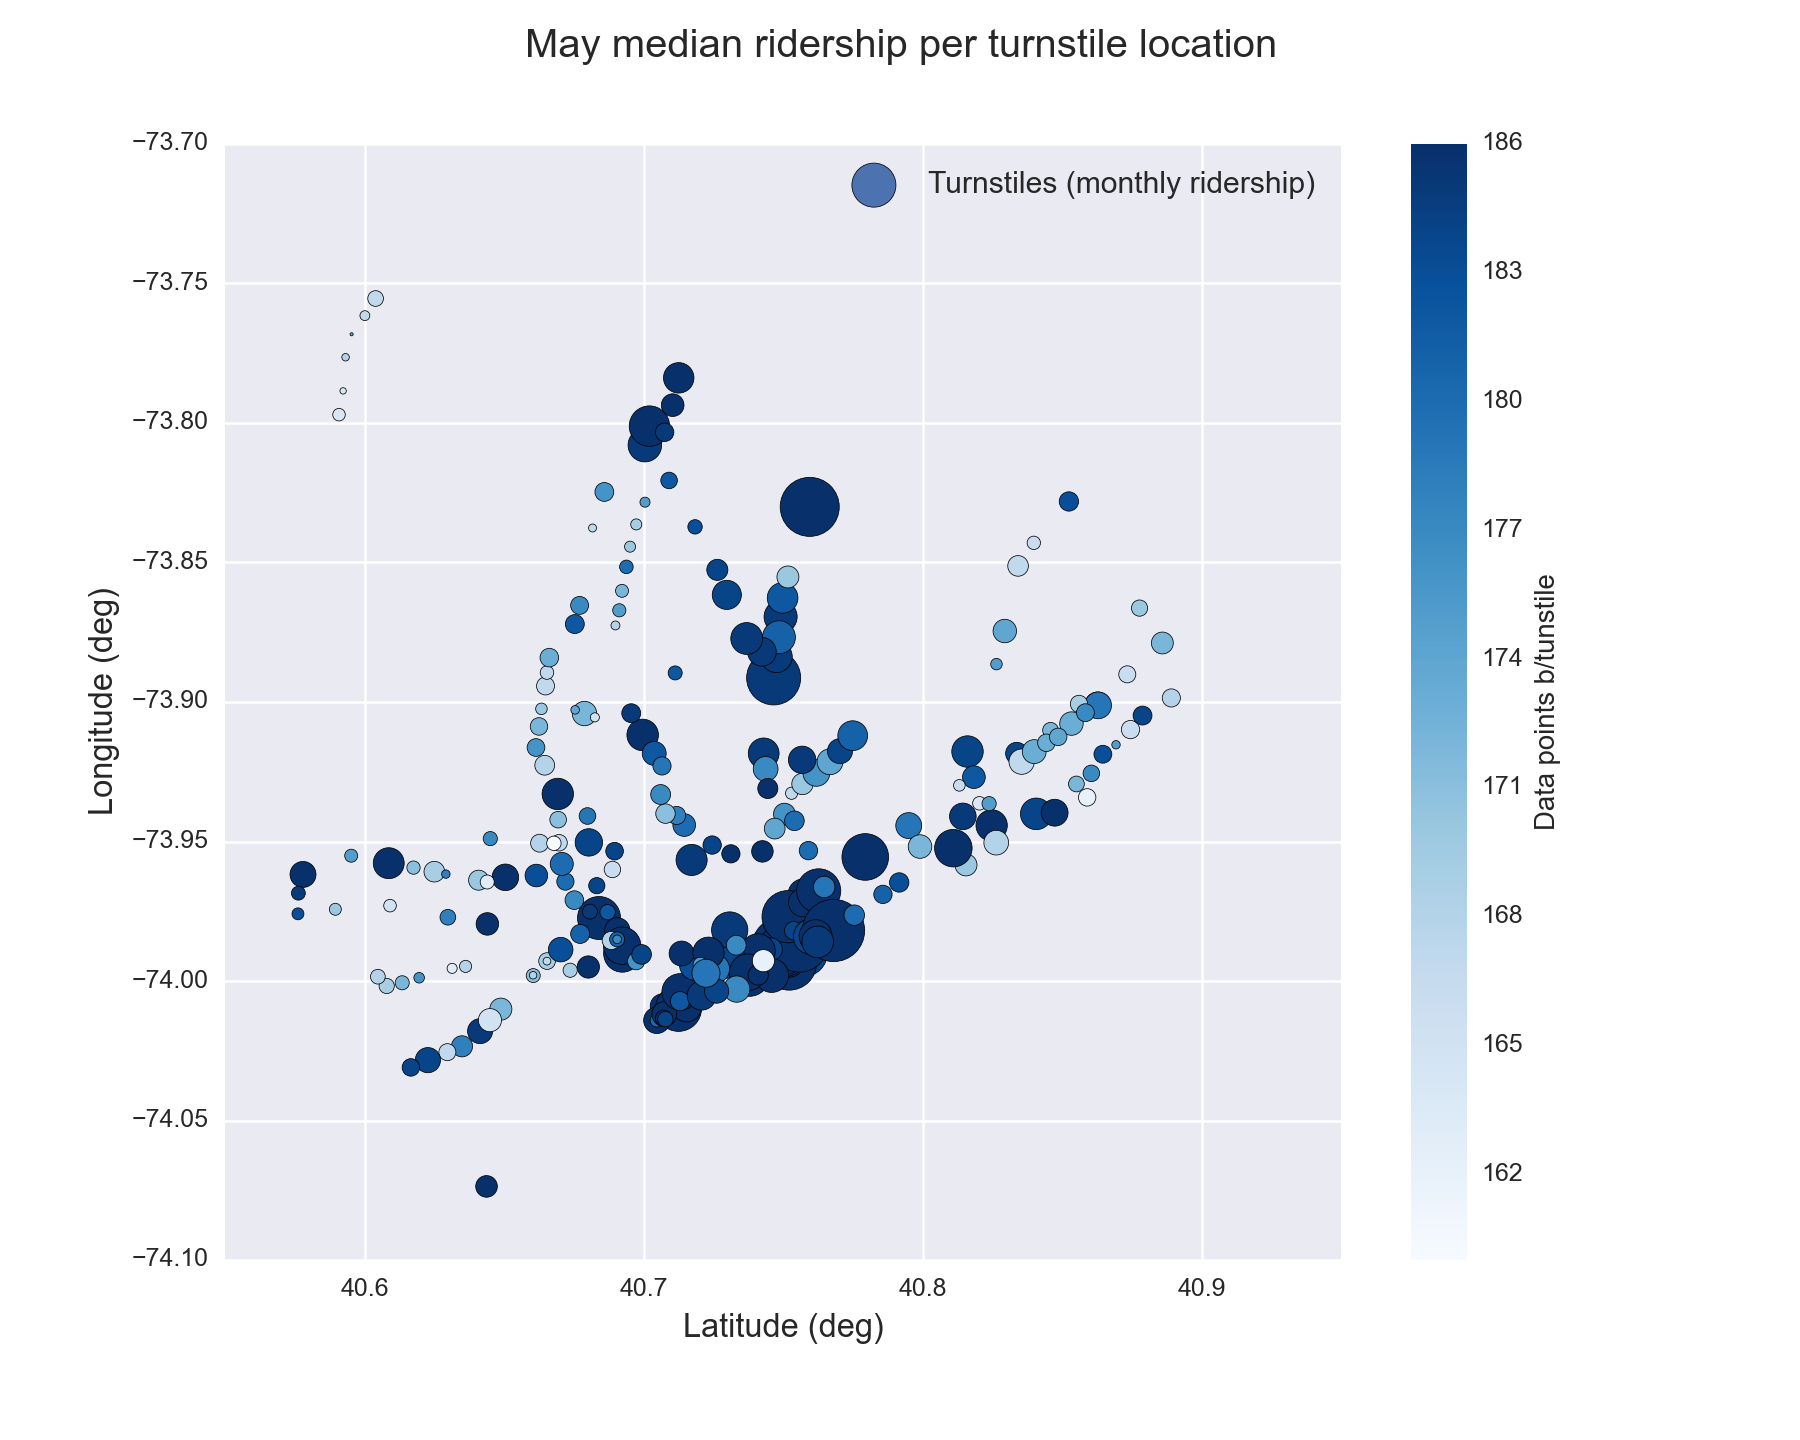
\includegraphics{medrider_loc.png}}
\caption{Turnstiles' locations within NYC, from the improved dataset.}\end{figure}

Besides the information provided by the NYC subway, the dataset also includes
weather information taken from several weather stations within the NYC area:
each turnstile, depending on the location in NYC, is merged with the weather
information of the closest weather station, thus providing temperatures, wind
speed, pressure, conditions, precipitations, etc.

The project focuses one main question: Does the weather conditions, specifically
precipitations, affect the NYC subway ridership? To answer this question we
will use exploratory tools, statistical tests and visualizations. Also, we will
try to fit a model to the data by choosing certain predicting features; will
the use of the precipitation variable improve the fit?


\section{Supporting Material}
\label{overview:supporting-material}
Within the project \href{https://github.com/itoledoc/IntroToDS}{github repository}
you will also find an ipython notebook, where most of the work done was recorded
for the readers reference.


\section{Some remarks about the datasets used}
\label{overview:some-remarks-about-the-datasets-used}
For this project we use the data set provided at Data Analyst Nanodegree's
portal for Project 1.

However, after the exploratory and data analysis, we created another dataset by
further munging the improved dataset. The basic idea was to smooth out features
that might be caused by individual turnstiles or measurements. To do this, we
grouped the data by time stamp and aggregated the entries by hour by adding all
the entries. Also, the precipitation information for each
time stamp was included by means of two columns:
\begin{itemize}
\item {} 
\code{rain\_hour}: indicator (0 or 1) for precipitations for the particular date
date and time. It is 1 if for any of the stations the conditions were Rain,
Light Rain, Hard Rain or Light Drizzle at that moment.

\item {} 
\code{rain\_day}: indicator (0 or 1) for precipitations for the particular day
of the report. If at any station of our turnstiles the conditions reported
precipitations during the day the value is set to 1.

\end{itemize}


\chapter{Statistical Test}
\label{section1:statistical-test}\label{section1::doc}
In lecture 3 and its problem set, the following question was given \emph{Do rainy}
\emph{days affect the ridership of the NYC subway?} To answer this problem we began
by creating two samples from our data:
\begin{itemize}
\item {} 
Sample A (\emph{No rain}) is a subgroup containing the entries where no rain was
reported, using the information of the \code{rain} variable (\(rain = 0\))

\item {} 
Sample B (\emph{Rain}) is a subgroup with the entries where some precipitation was
reported by means of the \code{rain} variable (\(rain = 1\))

\end{itemize}

By studying the distributions, using histograms, we were able to characterize
both data samples. We found out that both samples have a similar shape, clearly
not normal, and positively skewed ({\hyperref[section1:figure21]{\emph{figure 2.1}}}).
\begin{figure}[htbp]
\centering
\capstart

\scalebox{0.750000}{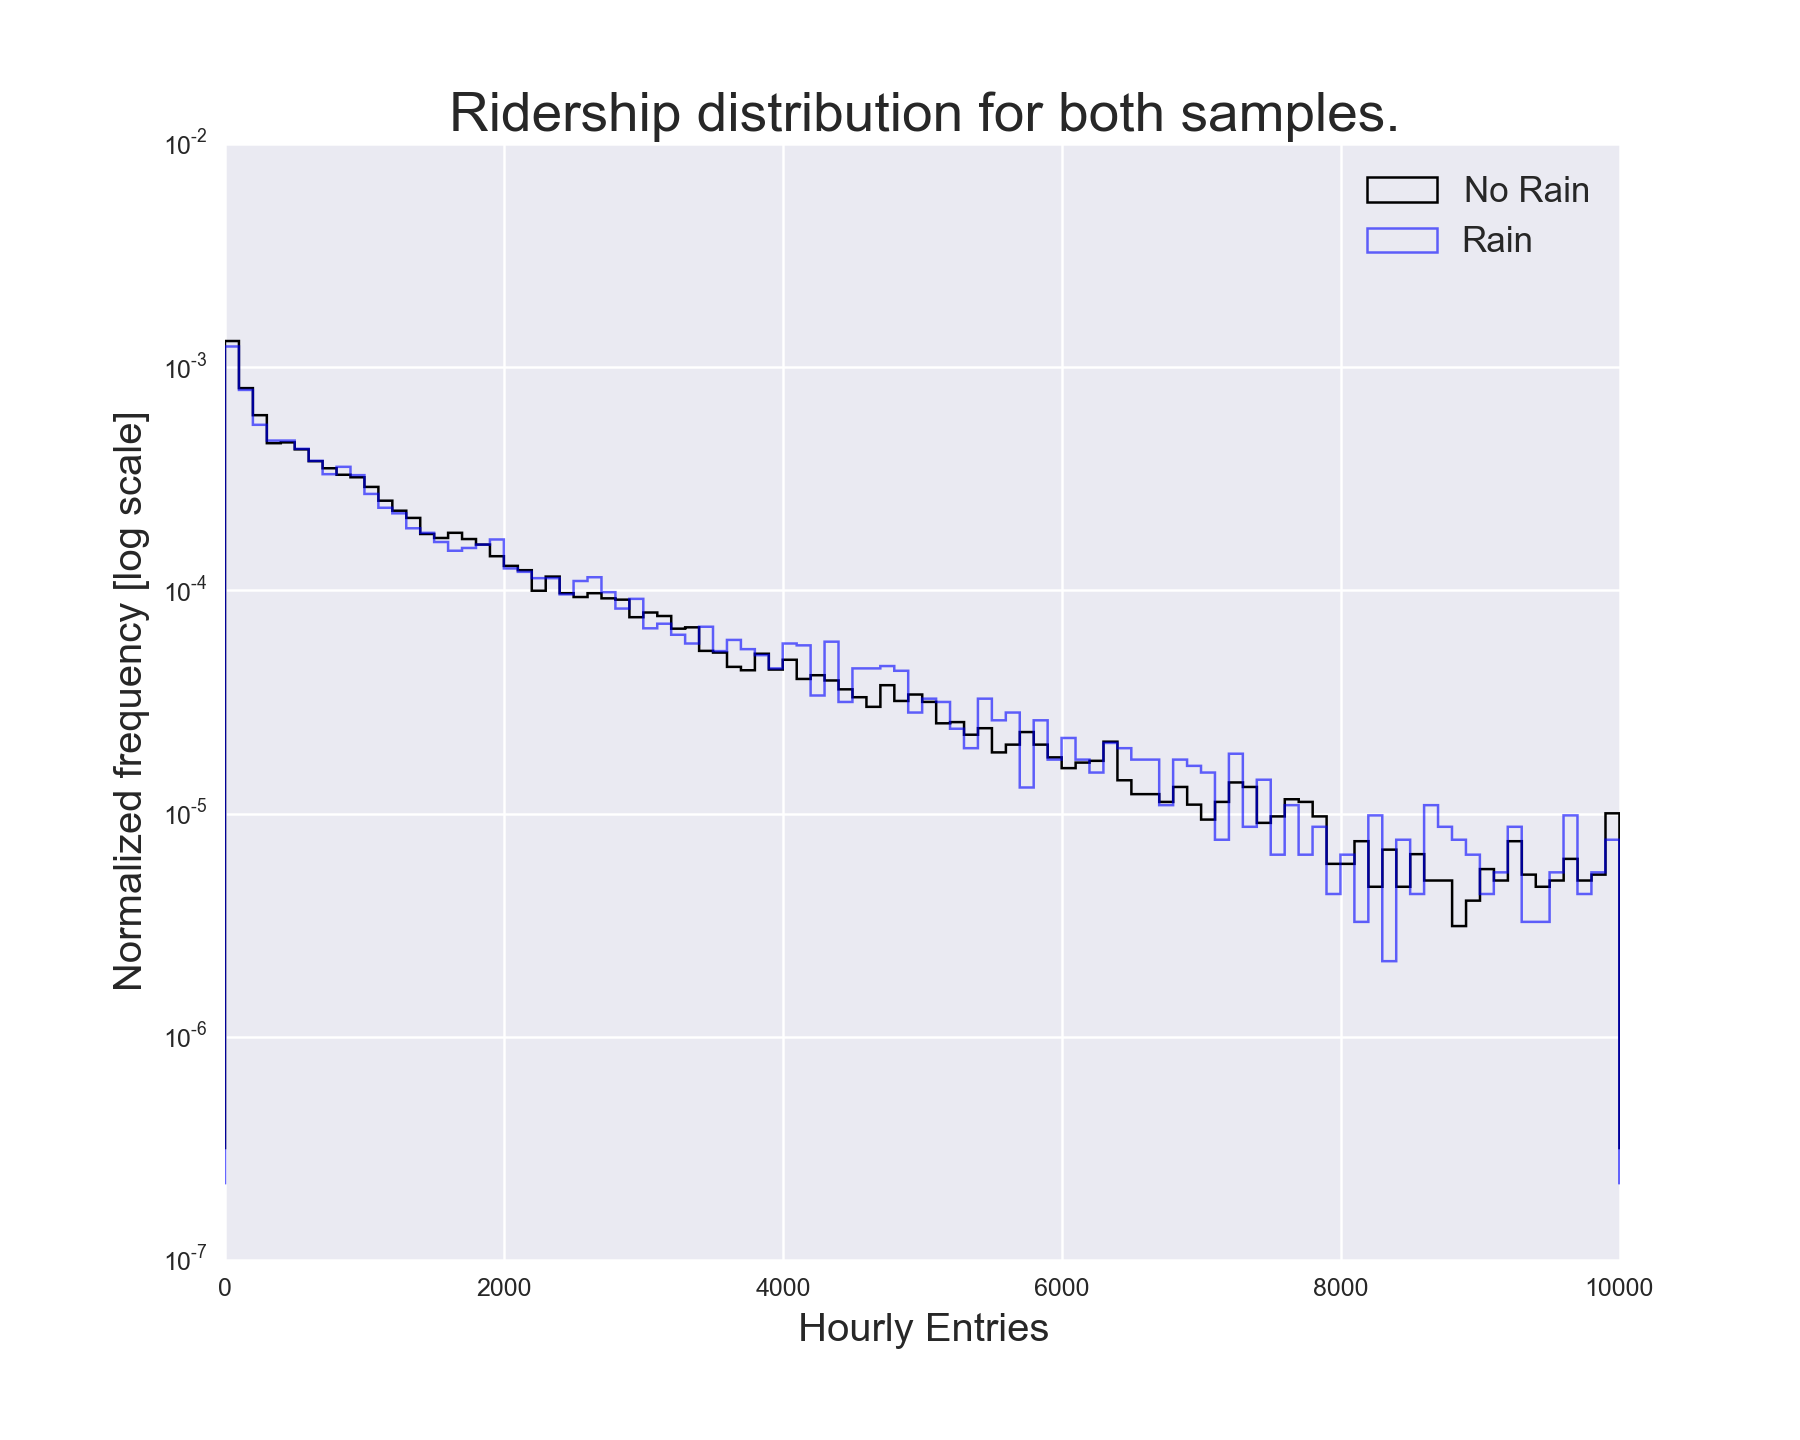
\includegraphics{samples_compared.png}}
\caption{Ridership distribution comparison between rainy and dry days.}{\small 
Please note the logarithmic scale on axis Y. It was used to allows us to
study the visualization with more detail.
}\label{section1:figure21}\end{figure}

Because of the non-normal distribution we decided to use the median as measure
of average for the samples:
\begin{itemize}
\item {} 
Sample A, days without precipitation, show a \textbf{median ridership of}
\textbf{901 passengers per hour.}

\item {} 
Sample B, rainy days, report a \textbf{median of 945 passengers per hour.}

\end{itemize}

To assess the significance of this result, that rain seems to increase ridership
in the NYC system by a small amount, we will use a non-parametric test.


\section{Statistical Test Used}
\label{section1:statistical-test-used}
\textbf{Which statistical test did you use to analyse the NYC subway data?}

The Mann Whitney U test {\hyperref[overview:wikimann]{{[}wikiMann{]}}} is chosen to assess the statistical
significance of this result.

\textbf{What is the null hypothesis}

The null hypothesis in our case is that both populations are equal, or that
there is no significant deviation on both
populations medians

\textbf{Did you use a one or two-tail P value?}

Because of the null hypothesis we will use a two-tail p-value.

\textbf{What is your p-critical value?}

We will use a p-critical equal to 0.05, meaning that in case the null hypothesis
is false we will require a 95\% of confidence.


\section{Justify the Statistical Test}
\label{section1:justify-the-statistical-test}
\textbf{Why is this statistical test applicable to dataset? In particular, consider}
\textbf{the assumptions that the test is making about the distribution of the ridership}
\textbf{in the two samples.}

The Mann Whitney U test, or Wilcoxon rank-sum test, is chosen because of
characteristics of our samples: we can't use a parametric test because the
distributions do not seem to follow any particular and well known probability
distribution which we could use to make inferences that could directly report
the significance of any difference between both populations.

The U test is particularly powerful to assess the significance of the difference
between the median of two samples that have similar distributions. The
assumptions that our data samples must comply with are basically:
\begin{itemize}
\item {} 
All observations of both groups are independent

\item {} 
The responses are ordinal (so we can use the ranking algorithm of the U test).

\end{itemize}


\section{Results}
\label{section1:results}
\textbf{What results did you get from this statistical test?}

We used the scipy implementation of the Mann Whitney U test
(scipy.stats.mannwhitneyu). The results from the test are:
\begin{itemize}
\item {} 
\(U = 150678745.0\)

\item {} 
\(p = 1.91 \cdot 10^{-6}\)

\end{itemize}

But the user should be aware that scipy reports a p-value for a one-tailed
hypothesis, so we multiply by 2 to get the significance for our hypothesis:
\begin{itemize}
\item {} 
\(p = 3.82 \cdot 10^{-6}\)

\end{itemize}

The averages from the two data samples have been already presented in the beginning
of this chapter.


\section{Interpretation and discussion}
\label{section1:interpretation-and-discussion}
\textbf{What is the significance and interpretation of these results?}

The interpretation, given the result from the U test, is that the the ridership
is not the same for rainy days than non-rainy days, with a significance higher
than 95\% (p \textless{} 0.05). Furthermore, from the descriptive statistics of our samples
we would conclude that the ridership tends to be higher in rainy days.

However we have limited ourselves here to follow the procedure suggested by the
lectures, assuming that observations of both groups are independent and there
no other factors that might wrongly induce this result. Even when the data sample
we use for the project has been through a more complete wrangling, there are
still some issues that might affect the results:
\begin{itemize}
\item {} 
There is missing data for several turnstiles. From the original sample of 240
turnstiles, only 52 have complete data for May; also, as discussed on the
forums, some precipitation data is missing from some weather stations.

\item {} 
We are using the variable \code{rain} to create our samples: this variable
indicates if the conditions at anytime of the day at a particular turnstile
were rainy. Is it the appropriate variable to use to build the subgroups?

\item {} 
There is one day which was a holiday (Monday 30th), should the data from this
day be discarded?

\end{itemize}

Let's look with more detail at some these problems.


\subsection{Missing data and precipitation distribution}
\label{section1:missing-data-and-precipitation-distribution}\begin{figure}[htbp]
\centering
\capstart

\scalebox{0.750000}{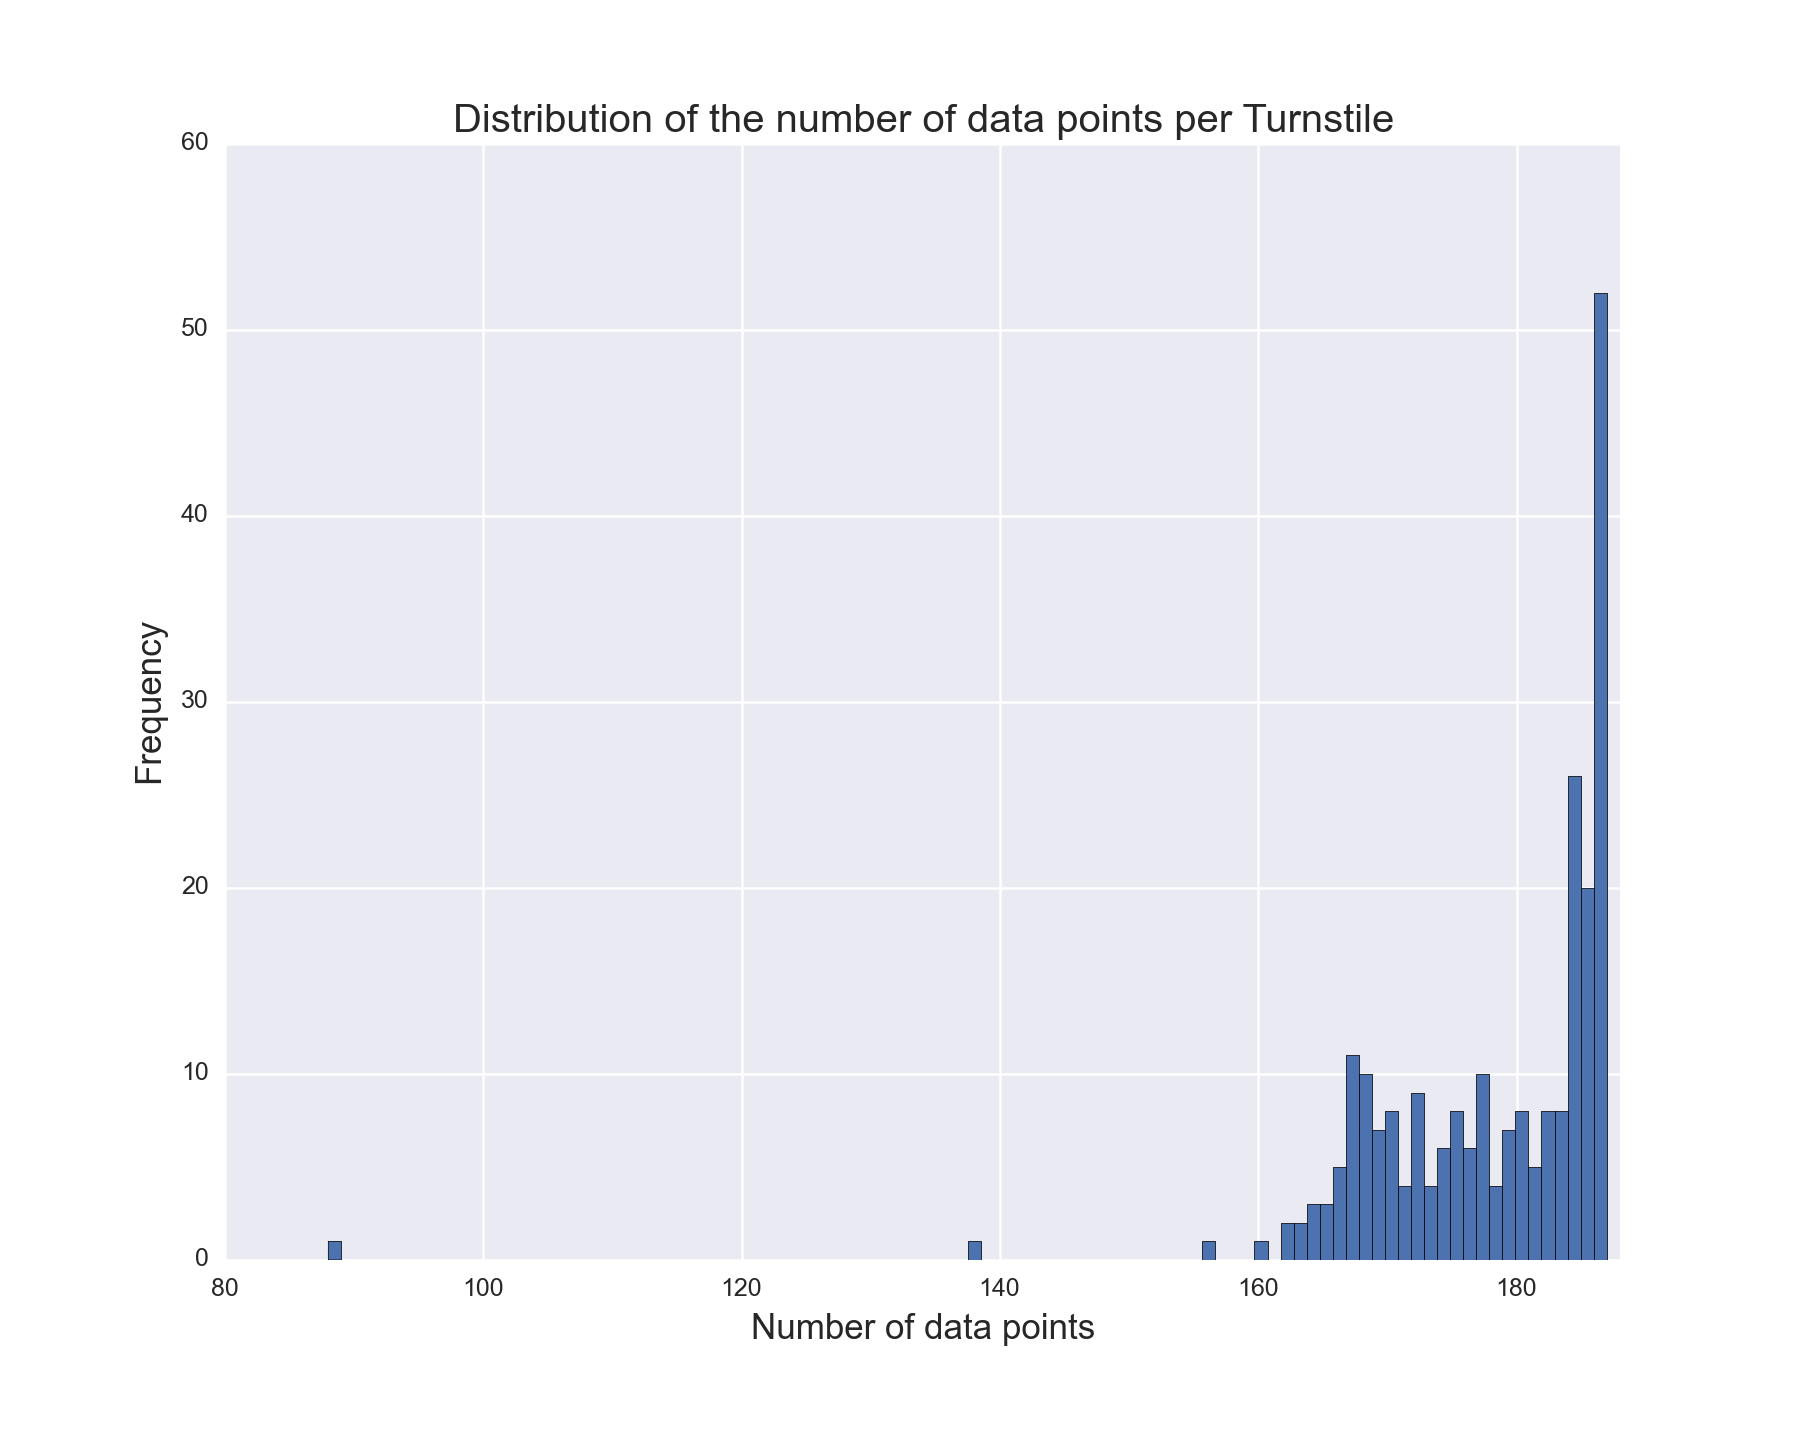
\includegraphics{dataentries.png}}
\caption{Number of data points (measurements) by turnstile on project's improved
dataset.}\label{section1:figure22}\end{figure}

{\hyperref[section1:figure22]{\emph{Figure 2.2}}} shows some turnstiles have missing data for the
month of May; with 31 days and 6 daily reports it is expected that a complete
monitored turnstile should have 186 measurements. This is the case for 52
turnstiles, but 185 turnstiles have a number of measurements between 160 and
185. 3 turnstiles had less than 160 entries, and after inspections they have
been removed because of the huge amount of missing data or time stamps
reporting 0 entries. Of the 185 turnstiles with incomplete data, there was one
case where at all time stamps the number of entries was 0, which was also
removed as it does not add any information to our analysis (even when in other
cases it could give further information).

The problem with the missing data is that, for some not clear explanation we
could provide, affects more the suburb stations turnstiles than the ones in
downtown areas. And suburb stations tend also to show lower number of hourly
entries, i.e, a lower ridership, than downtown turnstiles. This effect can be
seen in {\hyperref[section1:figure23]{\emph{Figure 2.3}}}.
\begin{figure}[htbp]
\centering
\capstart

\scalebox{0.750000}{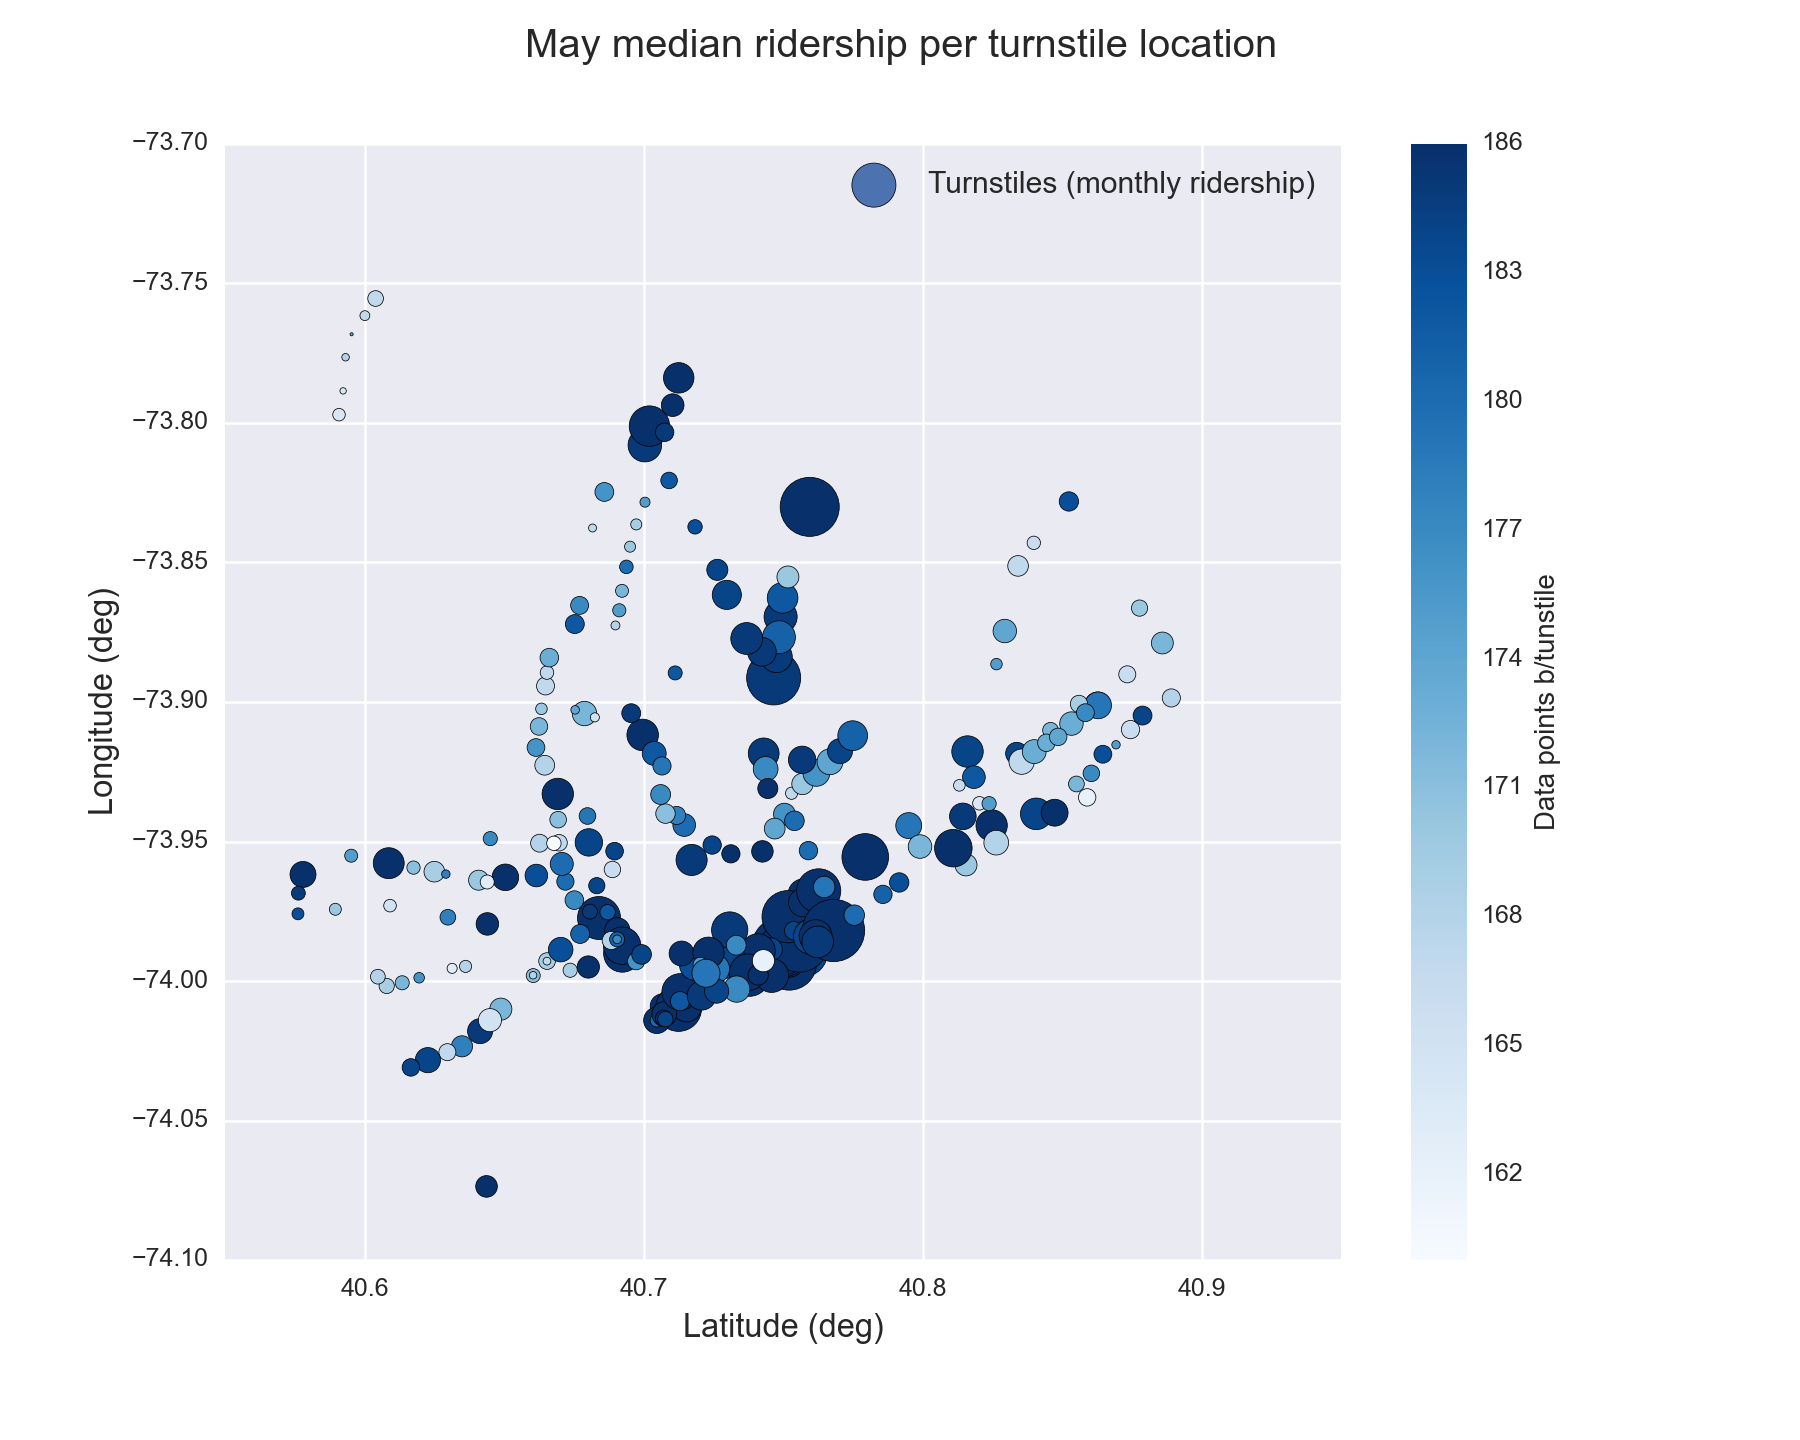
\includegraphics{medrider_loc.png}}
\caption{Turnstiles monthly median ridership, location and number of data points}{\small 
The figure shows the distribution of the turnstiles within NYC which are in
our dataset. The size is proportional to the monthly median ridership
(entries by hour) while the color indicates the data completeness of each
turnstile: whiter colors indicate locations with more missing data.
}\label{section1:figure23}\end{figure}

We wonder, as the reader also may, if this missing data could affect in anyway
our previous study. We are not completely sure, but we think that given the way
we performed our analysis it could happen that the results were affected: the
downtown station data, which also correspond to the group of stations with
higher ridership, is contributing to increase the median ``entries by hour'' that
we calculated, as they are located in the higher values side of the ridership
distribution. What happens if the stations in this locations are also the ones
that tend to have more rainy days? We didn't believe this was the case, but just
to be sure we created the plot shown in {\hyperref[section1:figure24]{\emph{Figure 2.4}}}.
\begin{figure}[htbp]
\centering
\capstart

\scalebox{0.750000}{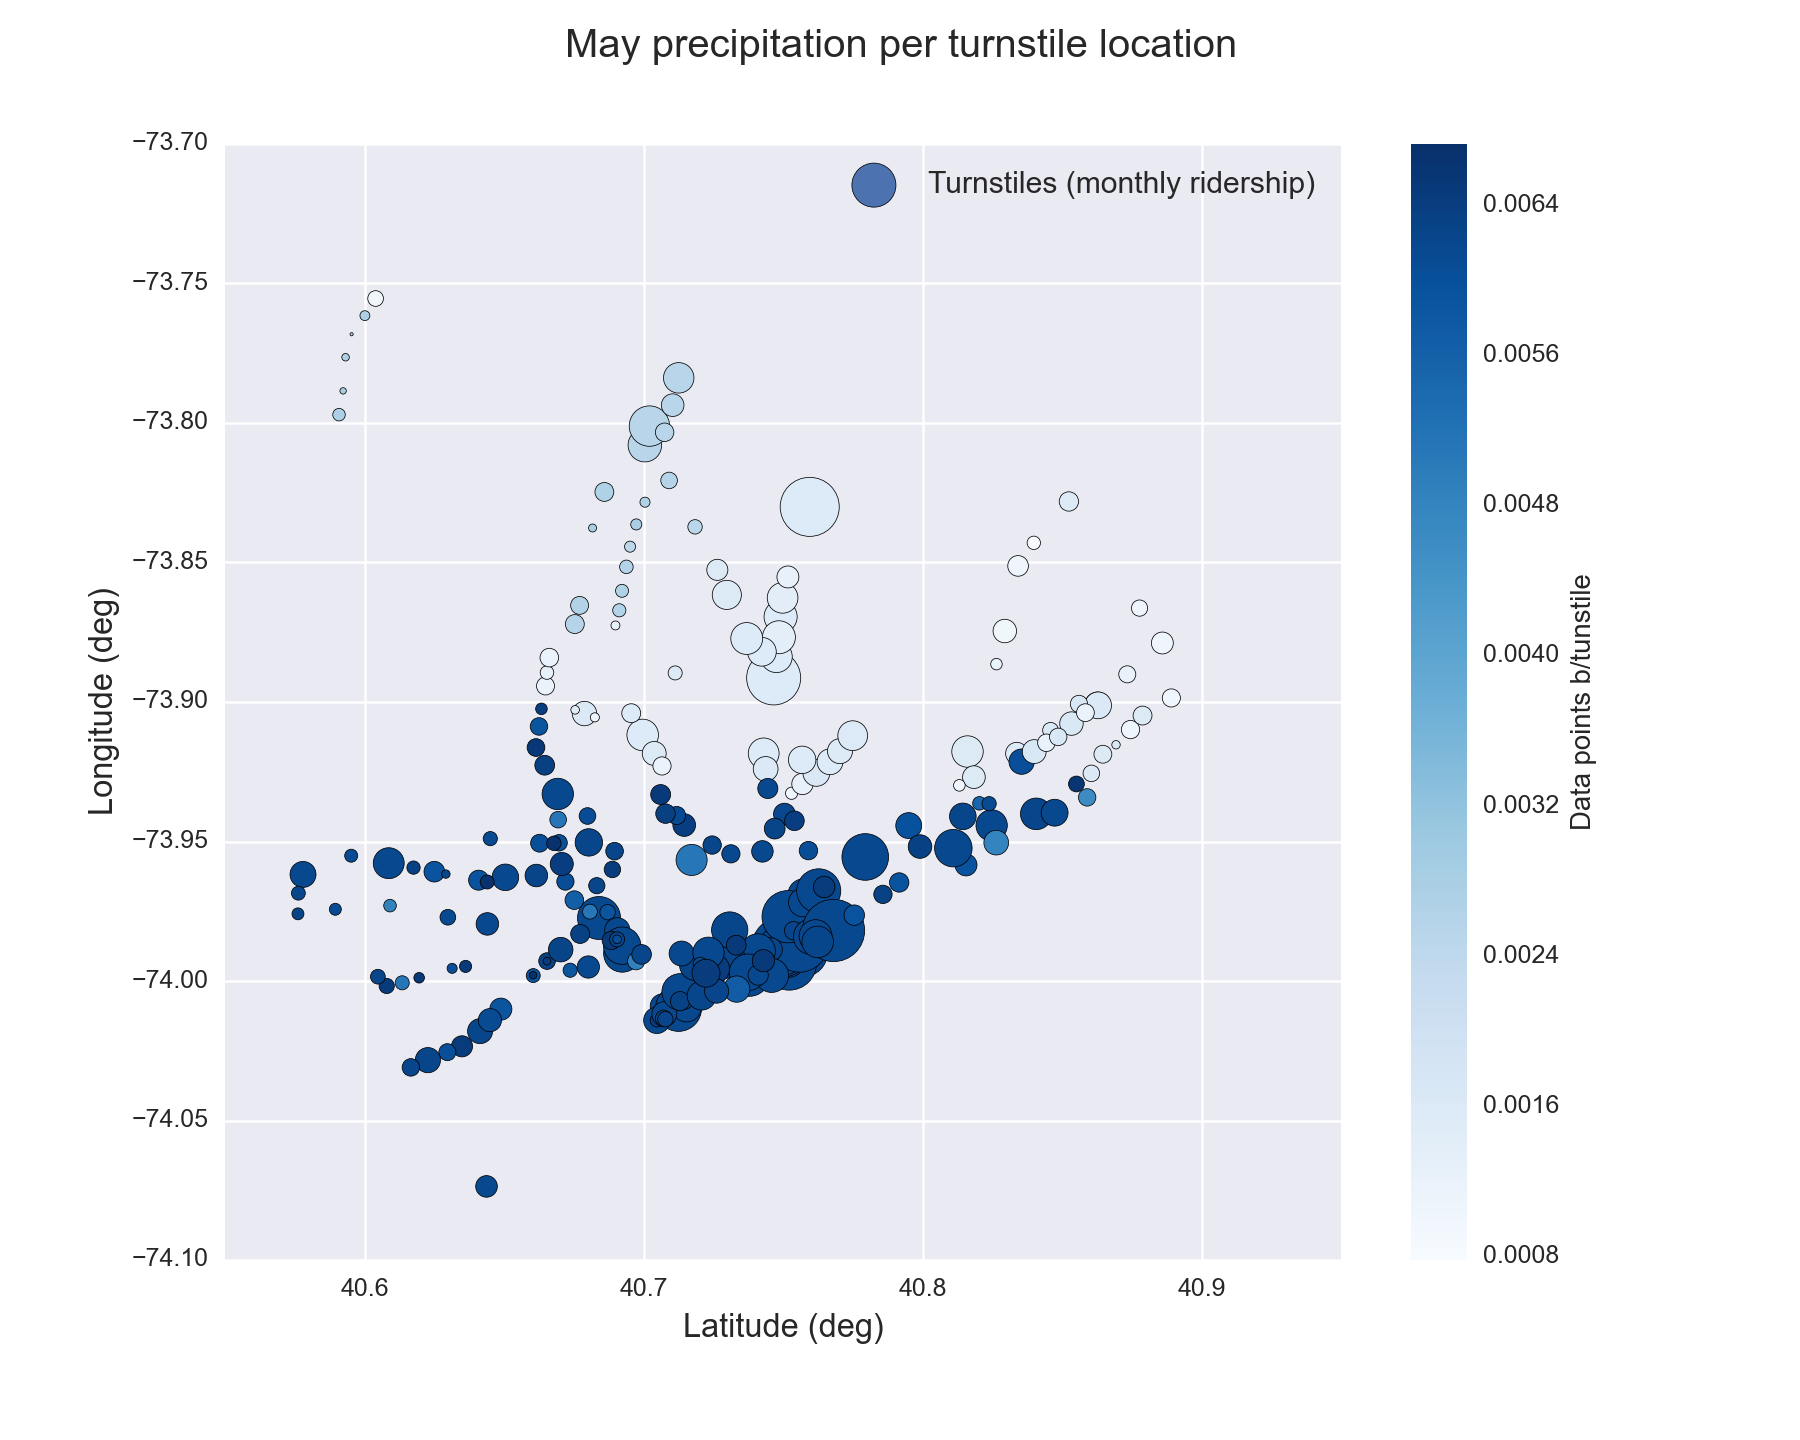
\includegraphics{medprecip_loc.png}}
\caption{Turnstiles monthly median ridership, location and mean precipitation.}{\small 
The figure shows the geographical distribution of the NYC turnstiles in the
project's improved dataset. Size is proportional to the monthly median
ridership and color represent the month's mean precipitation per turnstile.
The figure shows that precipitations are higher in southern (and downtown)
NYC.
}\label{section1:figure24}\end{figure}

The figure shows that the precipitation is higher in the northern NYC, which is
also the location of the most busy turnstiles: the median ridership of stations
with higher precipitation (\textgreater{} 0.004 inches) is 1116 entries by hour, while the
stations with lower precipitation (\textless{}= 0.004 inches) is 832 entries by hour. Also
the stations with higher precipitation report on average 7 rainy days while the
lower precipitation turnstiles only report 6 rainy days.


\subsection{The use of the \emph{rain} variable}
\label{section1:the-use-of-the-rain-variable}
The \code{rain} indicator in the improved data set reports if whether any
precipitation happened at the turnstile location during the day. Because some of
the precipitation data was missing in the weather tables, the conditions
reported in the \code{conds} variable were used to create the \code{rain} column (as
mentioned in the forums): if at anytime during a day the condition reported at
a turnstile location was one of the following the \code{rain} indicator was set to
one: `Rain', `Light Rain', `Heavy Rain' or `Light Drizzle'. This explains why
for 94 entries reporting \code{rain} equal to 1, the \code{meanprecipi} variable (mean
precipitation for the day at the location) was 0. Also, as shown before, this
indicator is different for each turnstile depending on the closest weather
station report. Thus, we find out that 216 turnstiles report 7 days of rain,
19 turnstiles report 6 rainy days, and 2 report 5 rainy days. Adding this
analysis with the one in the previous subsection, we have to be aware that the
samples might not be completely independent as previously thought.

Also, there is another important problem derived from the use of \code{rain} variable
that we hope to make clear with the plot shown on {\hyperref[section1:figure25]{\emph{Figure 2.5}}}.
\begin{figure}[htbp]
\centering
\capstart

\scalebox{1.000000}{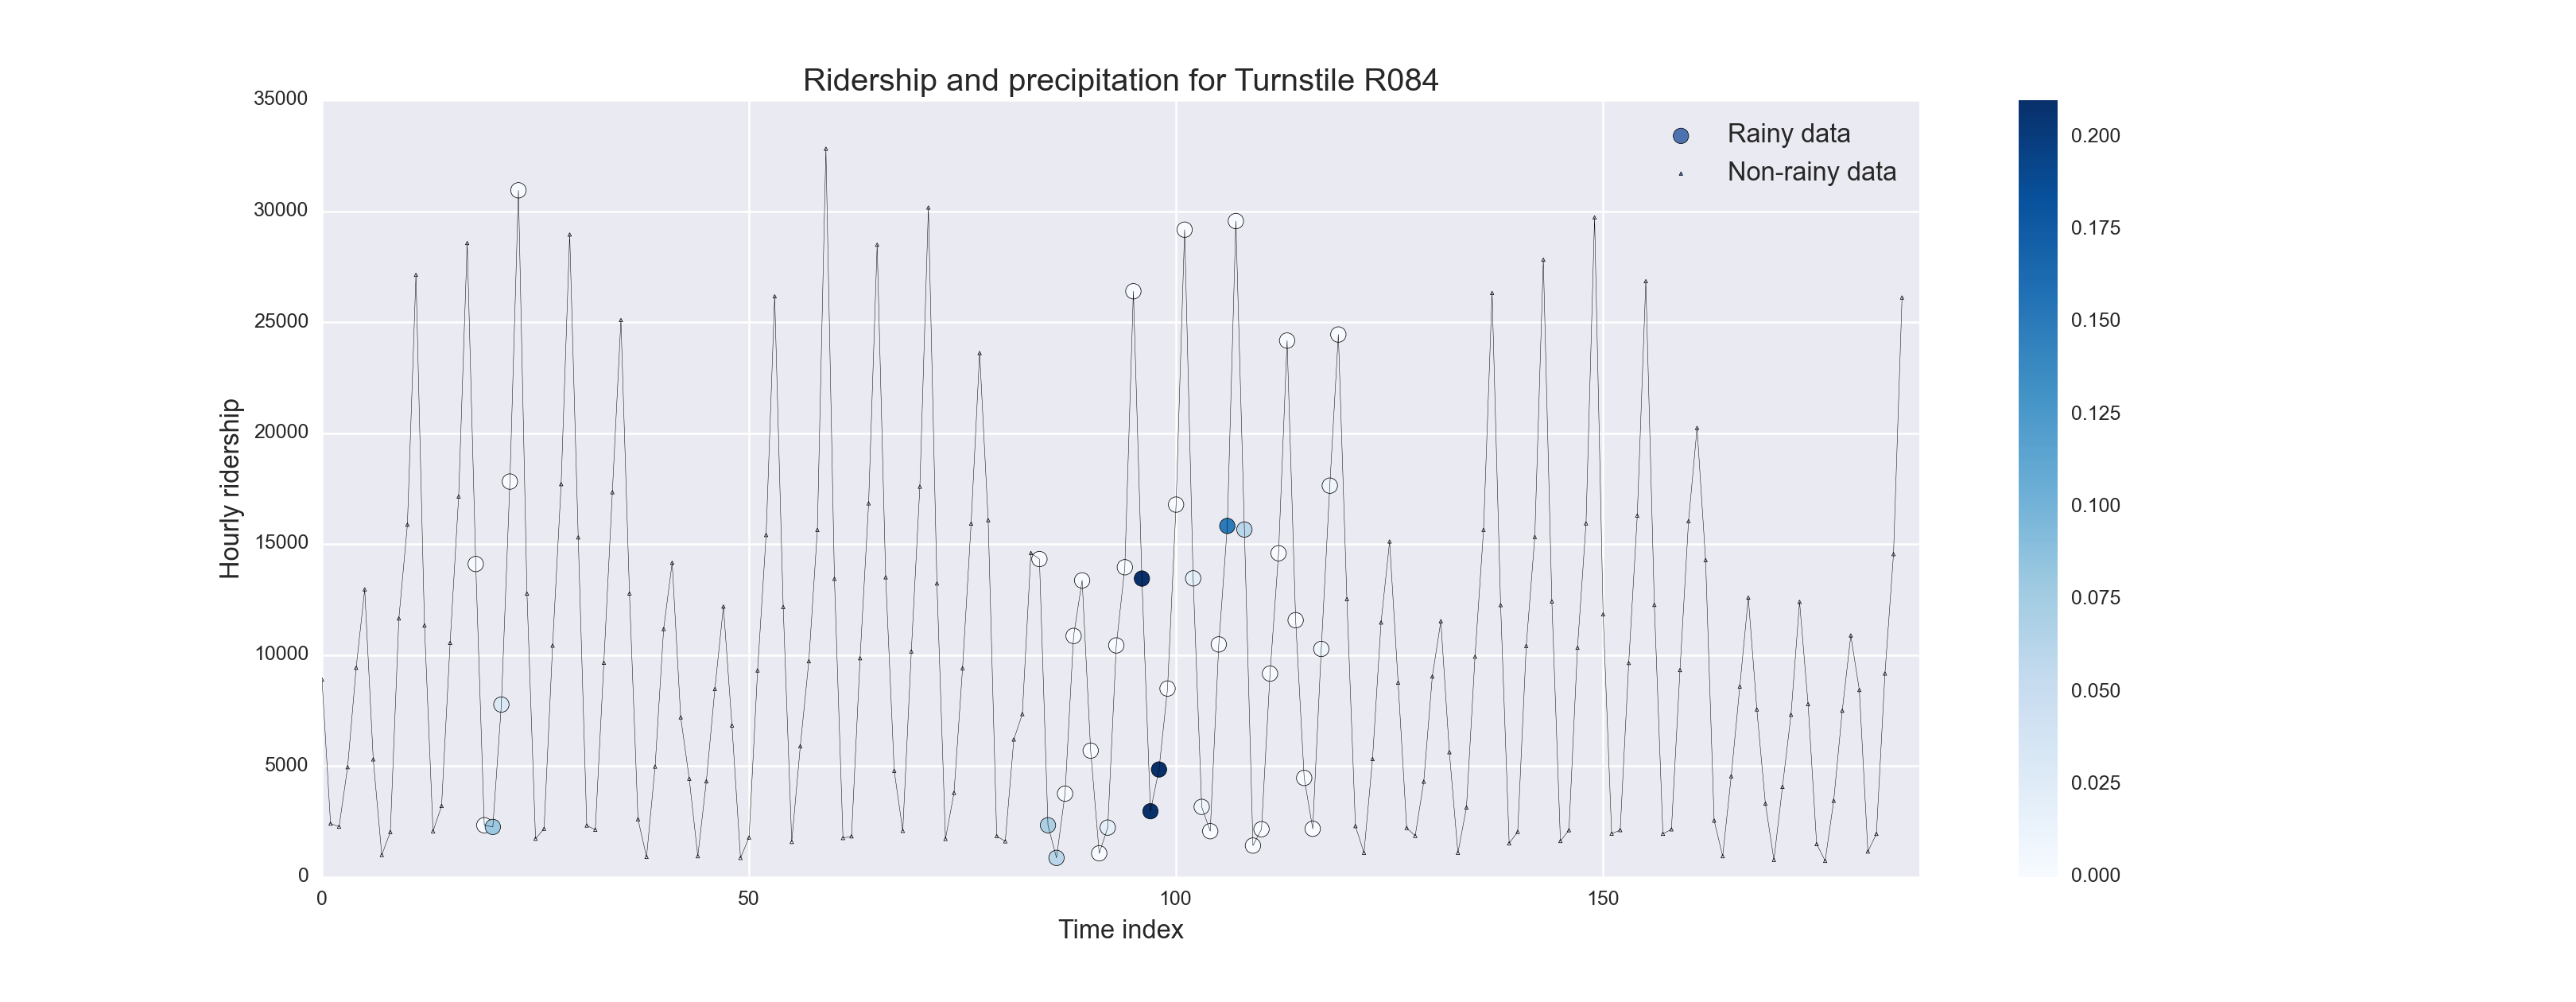
\includegraphics{r084.png}}
\caption{Ridership, precipitation and rain indicator for turnstile 084.}{\small 
The figure show the ridership evolution in May, in terms of entries per hour,
for turnstile 084, which is on one of the must busy stations in NYC subway.
There is one point every four hours for the month of May, and the symbols
indicate whether the day was rainy (big circles) or not rainy (small
triangles). Also, the precipitation amount in inches for the rainy days is
shown by means of the color bar in the right, with darker blue colors
indication more precipitation.
}\label{section1:figure25}\end{figure}

The problem we see on using the \code{rain} variable as and indicator of rainy
conditions for a turnstile is that a whole day is tagged as rainy even when only
rained at one time during the day. Furthermore, it can happen, as it can clearly
be seen on the figure, that the rain happened in one of the less busy hours of
the day, but still the whole day data will be tagged as rainy: this will clearly
affect the results of our previous analysis.


\subsection{Smoothing the data and answering the question again}
\label{section1:smoothing-the-data-and-answering-the-question-again}
In order to smooth out the previously mentioned effects we created a new data
set from where two samples will be created later. For this dataset we grouped
all individual turnstiles by time stamp, aggregating the ridership
(\code{ENTRIESn\_hourly}) using the \code{sum} function. In this way we have a set that
represent the behavior of the whole NYC subway as one system, instead of
individual turnstiles, reporting the total ridership at each time stamp. For
each time stamp a variable called \code{rain\_day} was created, which is 1 if in any
turnstile during a day within the whole NYC subway network reported some
precipitation, or 0 otherwise. Also, the data from May 30th is removed, since it
changes the statistic for the mondays. We will now redo the analysis using this
dataset, and in this way try to answer the original question:
\emph{Does the NYC subway ridership changes with the precipitation conditions?}
\begin{itemize}
\item {} 
Sample A is the subgroup of all the data coming from non rainy days
(\code{rain == 0}).

\item {} 
Sample B is the subgroup of the data in rainy days (\code{rain == 1}).

\end{itemize}

The ridership distribution of both samples are again similar in shape, but they
are not longer continuous, as show in {\hyperref[section1:figure26]{\emph{Figure 2.6}}}. We will use
again the median to report the average of each sample, and the Mann Whitney U
test to assess the significance of any difference we might found.
\begin{figure}[htbp]
\centering
\capstart

\scalebox{0.750000}{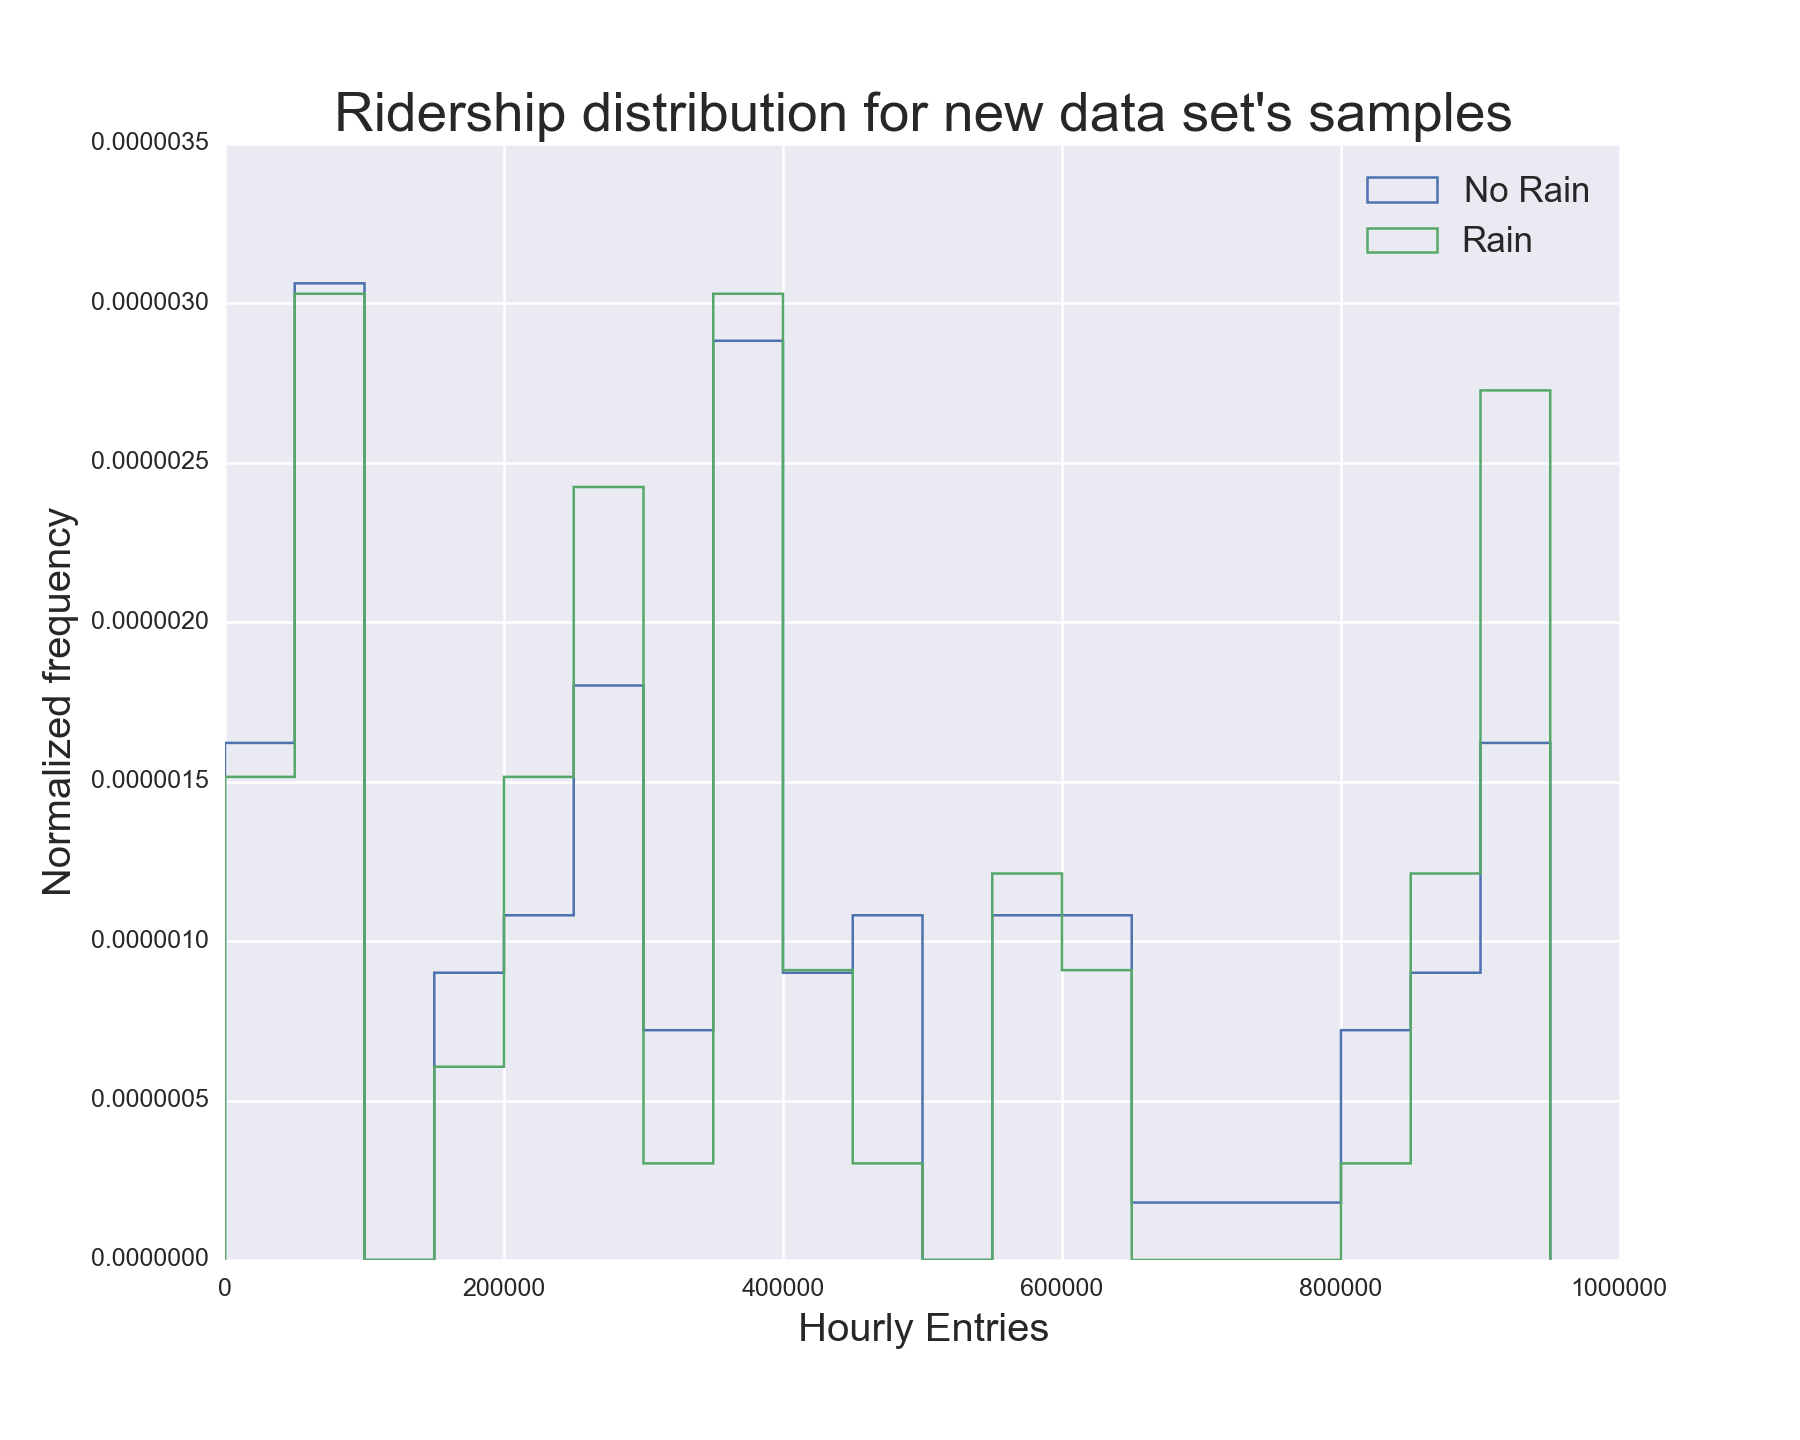
\includegraphics{samples2_compared.png}}
\caption{Ridership distribution comparison between rainy and dry days for the new
samples taken from the aggregated data.}\label{section1:figure26}\end{figure}

The ridership in non-rainy days has a \textbf{median of 370535 entries per hour},
while for rainy days the \textbf{median is 363124}. However the results from the U
test are now different:
\begin{itemize}
\item {} 
\(U \rm{statistic} = 3477.0\)

\item {} 
\(\rm{p-value} = 0.71\) (Two-tailed hypothesis)

\end{itemize}

So the difference in the medians are not significant now, and we can't conclude
that there is any meaningful difference in the ridership that could be explained
by the precipitation conditions.


\chapter{Linear Regression}
\label{section2:linear-regression}\label{section2::doc}
The second part of this work deals with the use of tools related to machine
learning: can we use the data to create models that will allows us to predict
the ridership based on some predicting features?

Problem Set 3 of the class has as one of the main goals the use of a linear
regression model that could help us to predict the ridership in the NYC subway.
We were asked to implement one of the algorithms that calculates the
coefficients of a multiple linear regression model: gradient descent. The
selection of the features, and thus the number of coefficients to fit, was left
as an exercise for the student.

After implementing the linear regression model, and study its strengths and
shortcomings, we used another algorithm to find the coefficients of the linear
regression model: OLS, or ordinary least squares.

Finally, a third method was used, also based on a linear regression algorithm,
but this time the model used higher order polynomials to learn from the data,
in an effort to deal with the nonlinearity of it.


\section{Linear regression algorithm(s)}
\label{section2:linear-regression-algorithm-s}
\textbf{What approach did you use to compute the coefficients theta and produce}
\textbf{prediction for ENTRIESn\_hourly in your regression model}


\subsection{Gradient descent}
\label{section2:gradient-descent}
The code used to implement the gradient descent algorithm to find the linear
regression coefficient can be checked on the python file available at the
github repository associated to this work (\code{projectone.py}), and on the
submissions to the \emph{Introduction to Data Science} class (problem set 3).


\subsection{Ordinary Least Squares (with statsmodels)}
\label{section2:ordinary-least-squares-with-statsmodels}
Selecting the same features as in the Gradient Descent exercise, we calculated
the coefficients of the linear model by using the OLS implementation of the
statsmodels python library {\hyperref[overview:statsmodels]{{[}statsmodels{]}}}.


\subsection{Polynomial features with Ridge linear regression}
\label{section2:polynomial-features-with-ridge-linear-regression}
After analysing the results from the previous regressions, and for reasons that
will become clear after the description of their results, we went a little
further and we used a polynomial transformation of the selected features, and
another linear regression algorithm, the Ridge regression, was used to find the
coefficients and predict ridership. The model used and results will be shown in
the interpretation section.


\section{Models and features used}
\label{section2:models-and-features-used}
\textbf{What features (input variables) did you use in your model? Did you use any}
\textbf{dummy variables as part of your features?}

The selection of the features to use and how to use them in the model was not
a linear process, but an iterative work based on exploratory statistics,
residuals analysis and study of the models obtained to predict the ridership.
In fact, for the problem set 3 in the class we used a different set of variables
as predictors (specifically \code{day\_week} instead of \code{weekday}).

Also, it was because of these iterative analysis that we decided to give a try
to a third method to model the data which included the use of polynomial
features.

The multiple regression model used for the first two methods can be written as:
\phantomsection\label{section2:multreg-mod}\phantomsection\label{section2:equation-multreg_mod}\begin{gather}
\begin{split}\hat y = \theta_0 + \theta_1 x_1 + theta_2 x_2 + ... + \theta_k x_k\end{split}\label{section2-multreg_mod}
\end{gather}
where \(\hat y\) is the predicted variable, \(x_i\) are the predictors
(features) and \(\theta_i\) are the coefficients or parameters that we are
looking for using either the gradient descent or the OLS algorithms.

For our work we decided to use the following predictors:
\begin{itemize}
\item {} 
\code{UNIT}: turnstile unique identification. The use of the identification
of each turnstile starts from the realization that the turnstiles have
different ridership volumes for the same time periods, as it can be readily
seen by comparing ridership averages. However this is a non-numerical
categorical variable, so it was required to transform this variable to a
numerical format by using dummy variables. This steps adds at once \emph{n} extra
features or predictors, one for each turnstile in our data, which adds a lot
of computing work to the algorithm.

\item {} 
\code{hour}: numerical variable that indicates the hour of the day when the
ridership is reported for each turnstile. This variable can takes values that
are continuous between 0 and 24, even when in the improved dataset the
observed values are reported every four hours; it adds one coefficient to
the calculations. {\hyperref[section2:figure31]{\emph{Figure 3.1}}} shows the relation of the
ridership values with hour the day.

\end{itemize}
\begin{figure}[htbp]
\centering
\capstart

\scalebox{0.800000}{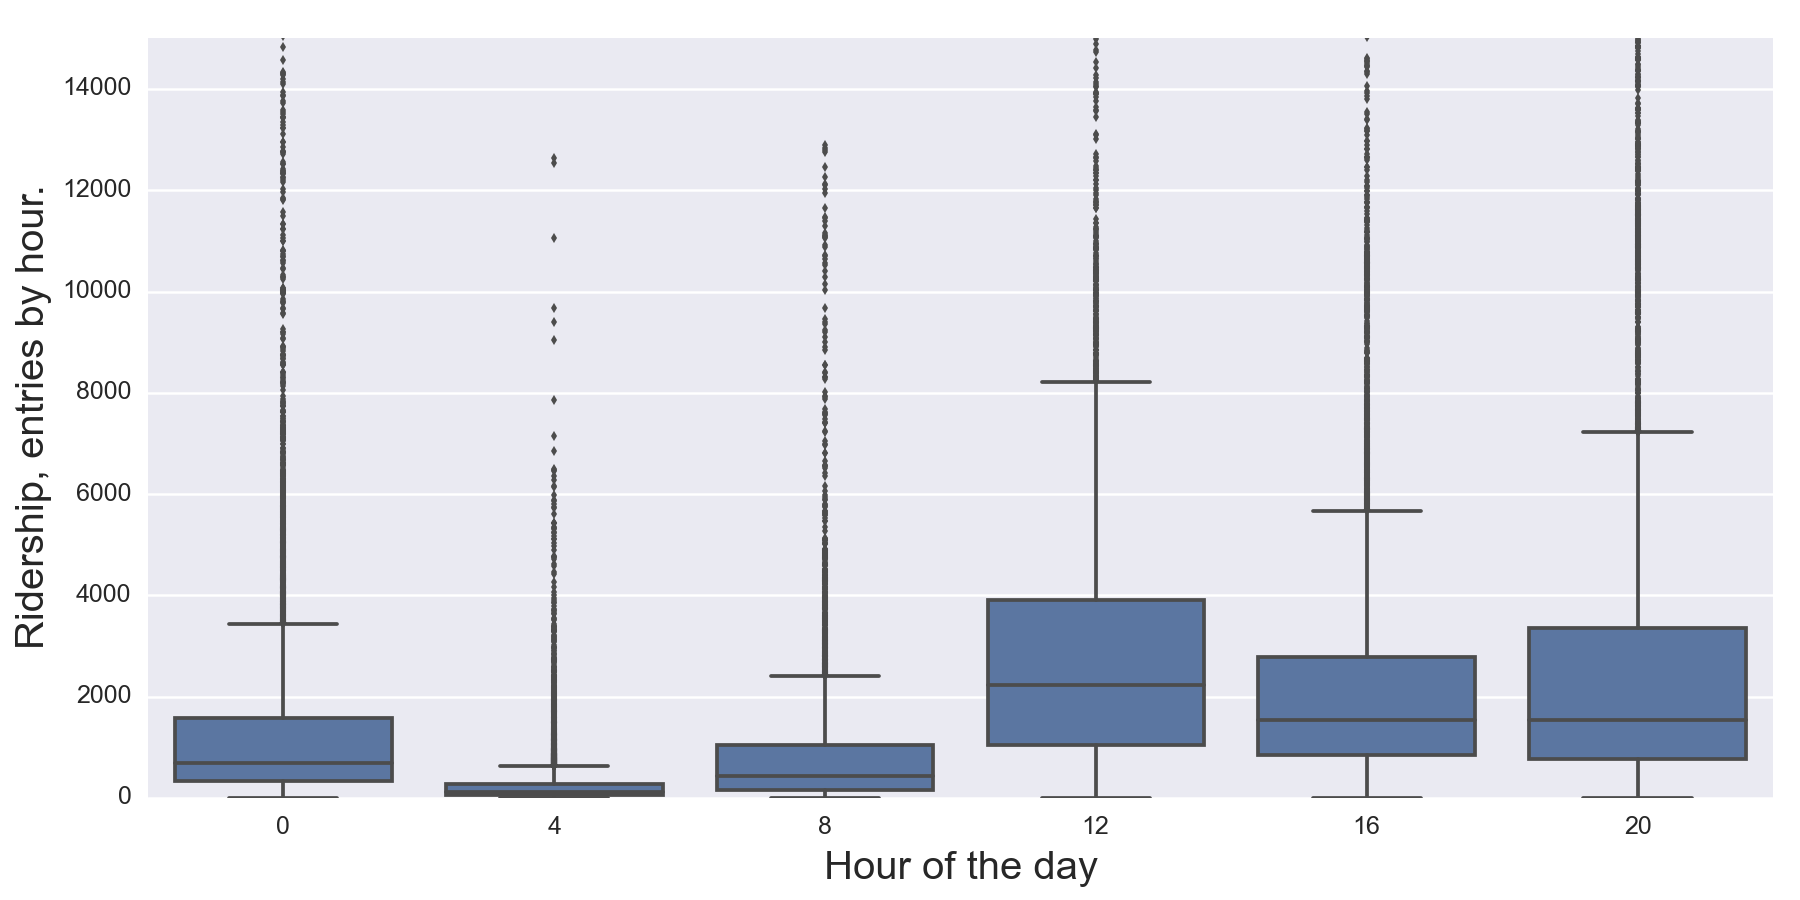
\includegraphics{hour_rider.png}}
\caption{Ridership vs hour of the day.}{\small 
Instead of just constructing a scatter plot, we decided to use another
descriptive statistic method to study the relation, if any, between ridership
and hour of the day. We used boxplots to visualize the distribution of
ridership for each hour of the day. In this way we can see that the medians
do not follow a linear relation with the hour of the day, and that there is a
huge spread of possible ridership values for each hour.
}\label{section2:figure31}\end{figure}
\begin{itemize}
\item {} 
\code{weekday}: numerical (and categorical) variable indicating if the day when
the ridership measurement was done was either a weekday (1) or weekend day (0).
{\hyperref[section2:figure32]{\emph{Figure 3.2}}} shows the relation of the ridership with kind of
day.

\end{itemize}
\begin{figure}[htbp]
\centering
\capstart

\scalebox{0.800000}{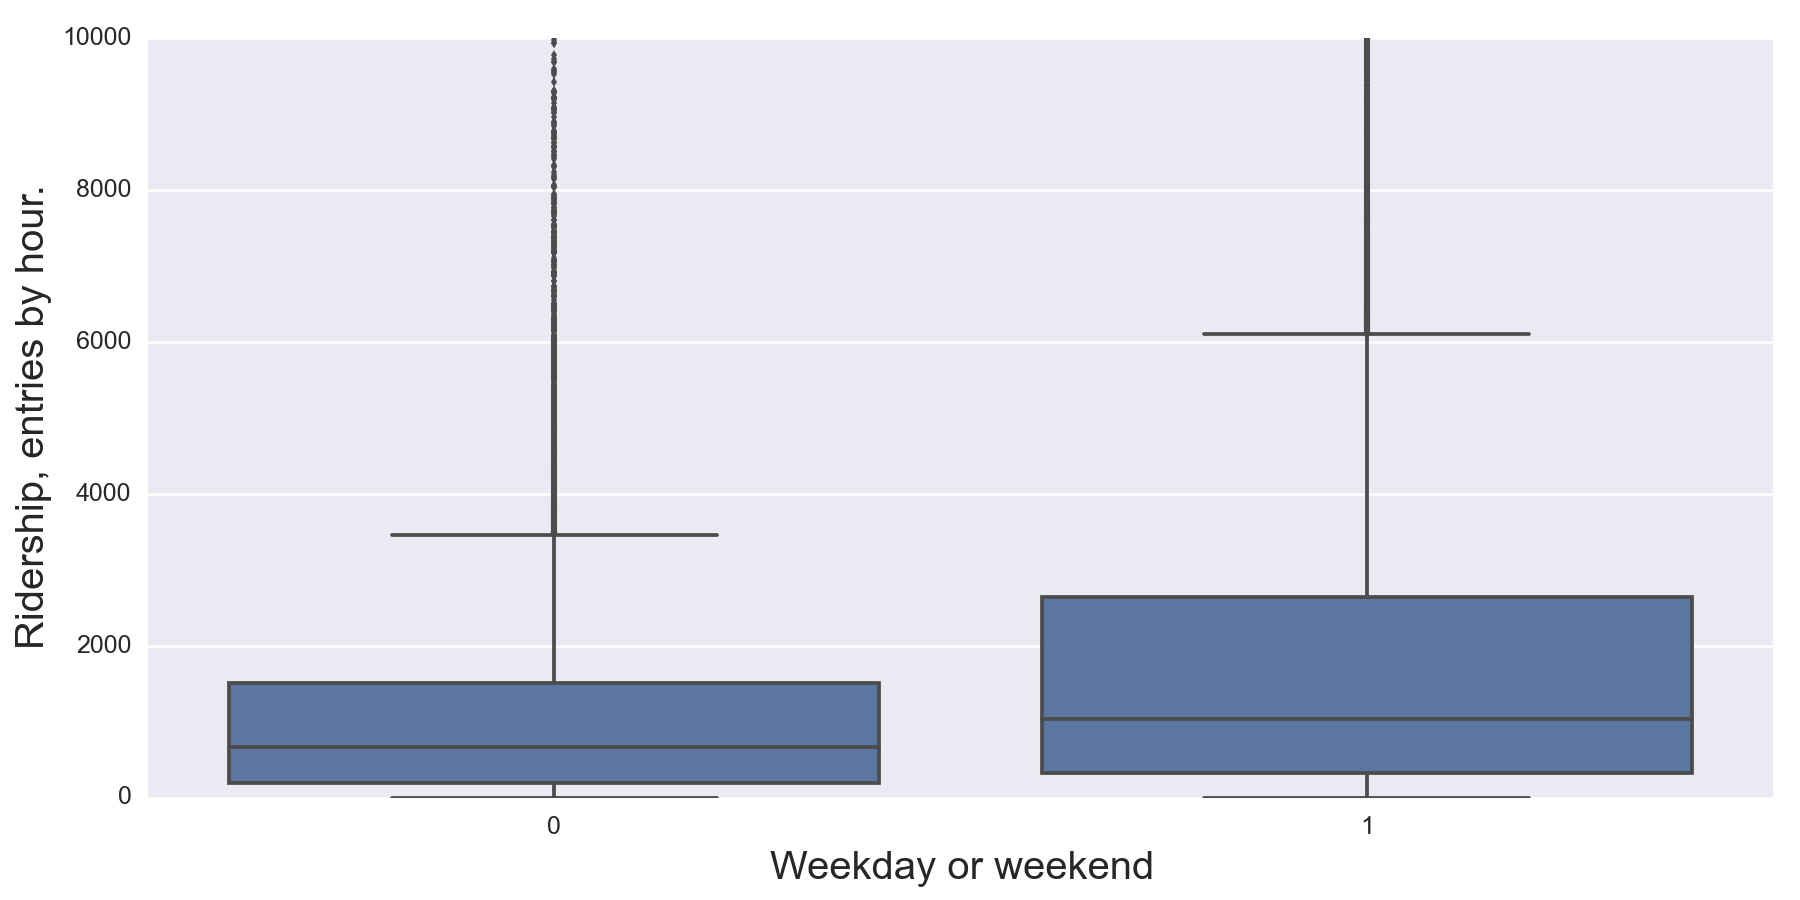
\includegraphics{weekday_rider.png}}
\caption{Ridership vs weekday/weekend-day.}{\small 
This plot show the ridership distribution as boxplots for work days (Monday
to Friday) and weekend days (Saturdays and Sundays). It is clear that even
when the spread in entries per hour is still big a linear correlation can
be used.
}\label{section2:figure32}\end{figure}
\begin{itemize}
\item {} 
\code{rain}: daily precipitation condition for a turnstile location (0 for a clear
day, 1 for rainy). Even when is a categorical variable, it is also numerical,
and it is used as the final predictor feature for our linear model.
{\hyperref[section2:figure33]{\emph{Figure 3.3}}} shows the relation of the ridership values with
precipitation conditions.

\end{itemize}
\begin{figure}[htbp]
\centering
\capstart

\scalebox{0.800000}{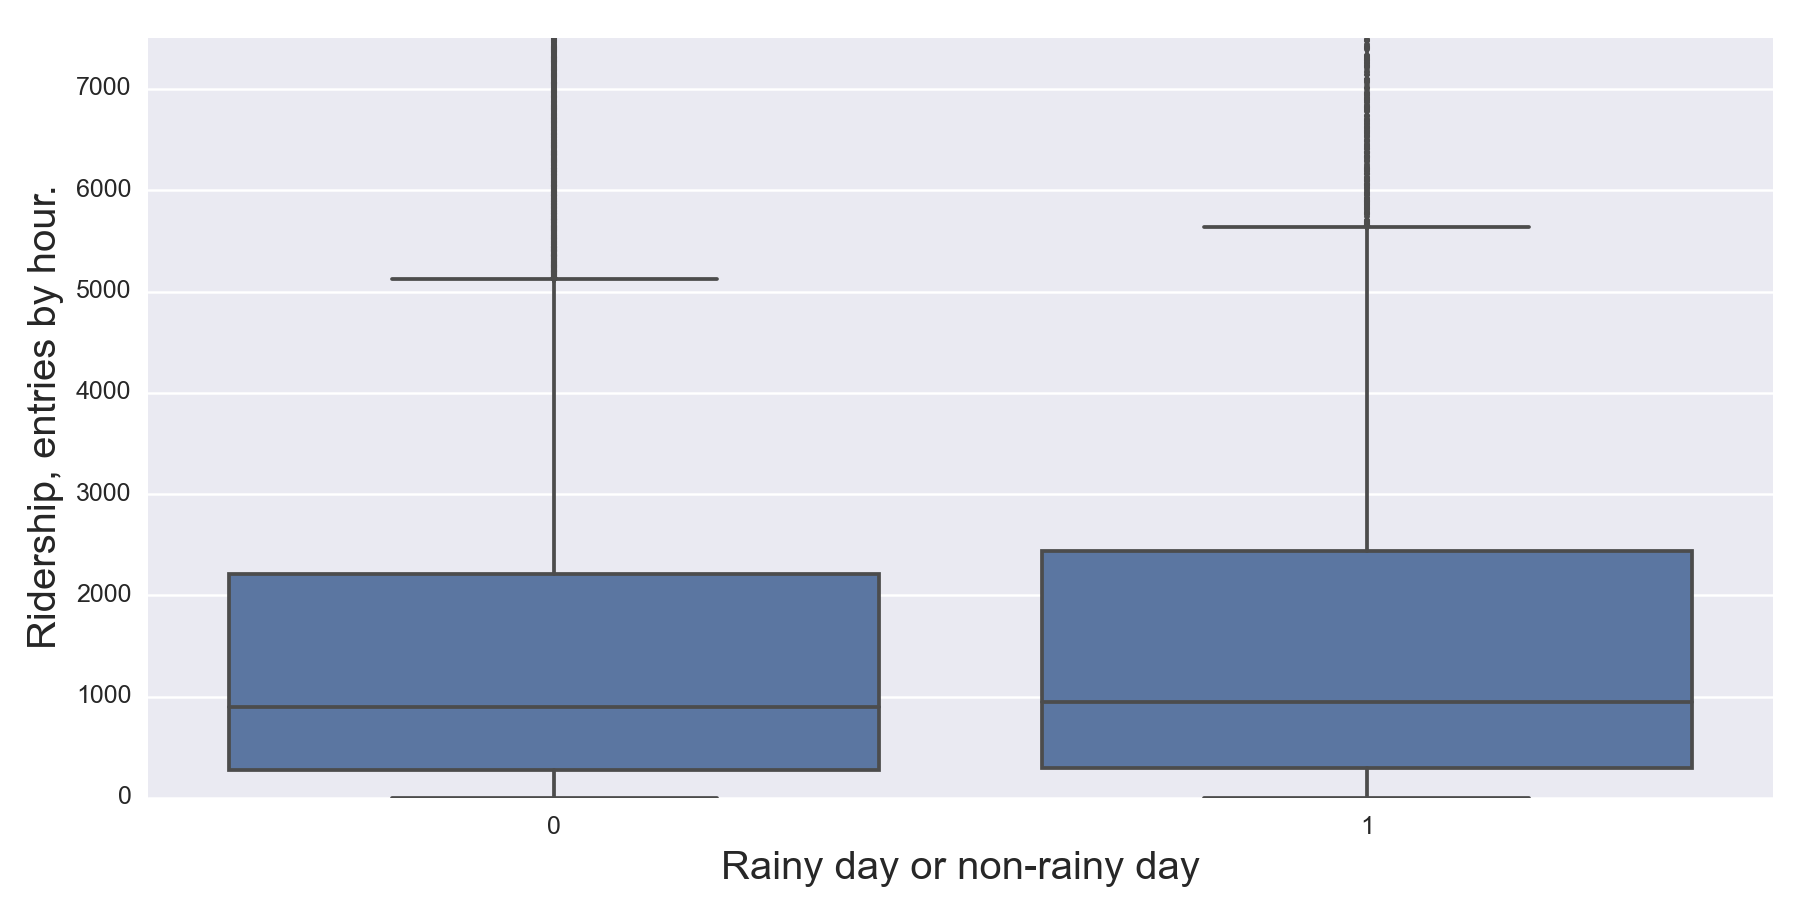
\includegraphics{rain_rider.png}}
\caption{Ridership vs rainy conditions.}{\small 
With the use of boxplots again, we can see in this figure that a really mild
linear correlation exist between daily precipitation conditions and
ridership. (Which as was shown in the previous section is not significant).
}\label{section2:figure33}\end{figure}

\textbf{Why did you select these features in your model?}

The features were selected based partially on intuition and partially by
exploratory analysis. First, it was clear that the behavior for each individual
turnstile was mainly a function of the hour of the day and the day of the week,
as is shown in {\hyperref[section2:figure34]{\emph{Figure 3.4}}}: there is a clear periodicity in the
ridership behavior for each day, depending on the time of the day, and also a
dependence on the day of the week. However the relation is clearly non-linear.
We kept the \code{hour} as a predictor because is an important predictor, an in a
very rough approximation one can see that ridership is lower in the beginning
of the day while reaching a peak on the evenings.
\begin{figure}[htbp]
\centering
\capstart

\scalebox{1.000000}{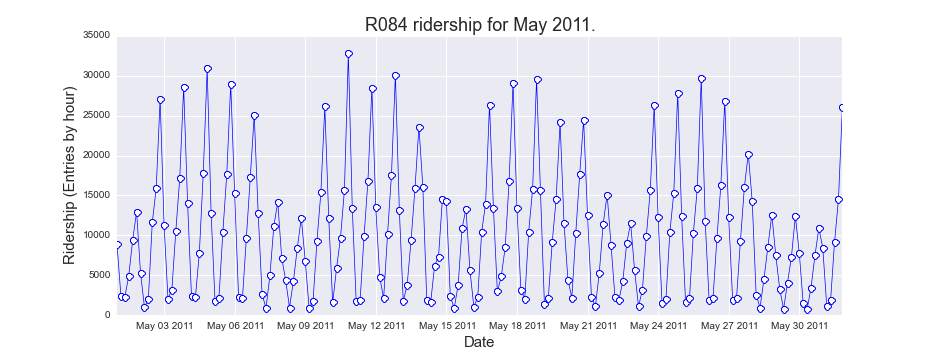
\includegraphics{r084_may.png}}
\caption{Ridership vs date for turnstile R084.}{\small 
The figure clearly shows a periodic behavior for the ridership behavior for
a particular turnstile, which is a function mainly of the hour of the day and
day of the week. Ridership peaks are usually seen at 20 hours, while weekends
and holidays (May 30th) being less busy than weekdays.
}\label{section2:figure34}\end{figure}

However, we decided to use \code{weekday} instead of \code{day\_week} (the second being the
day of the week, i.e, a number between 0 and 6, where 0 is Monday and 6 Sunday),
because the major change on ridership behavior is seen between work days and
off days (weekends), and \code{weekday} can be better modeled by a linear model than
\code{day\_week} (as it can be checked on {\hyperref[section2:figure35]{\emph{Figure 3.5}}})
\begin{figure}[htbp]
\centering
\capstart

\scalebox{0.800000}{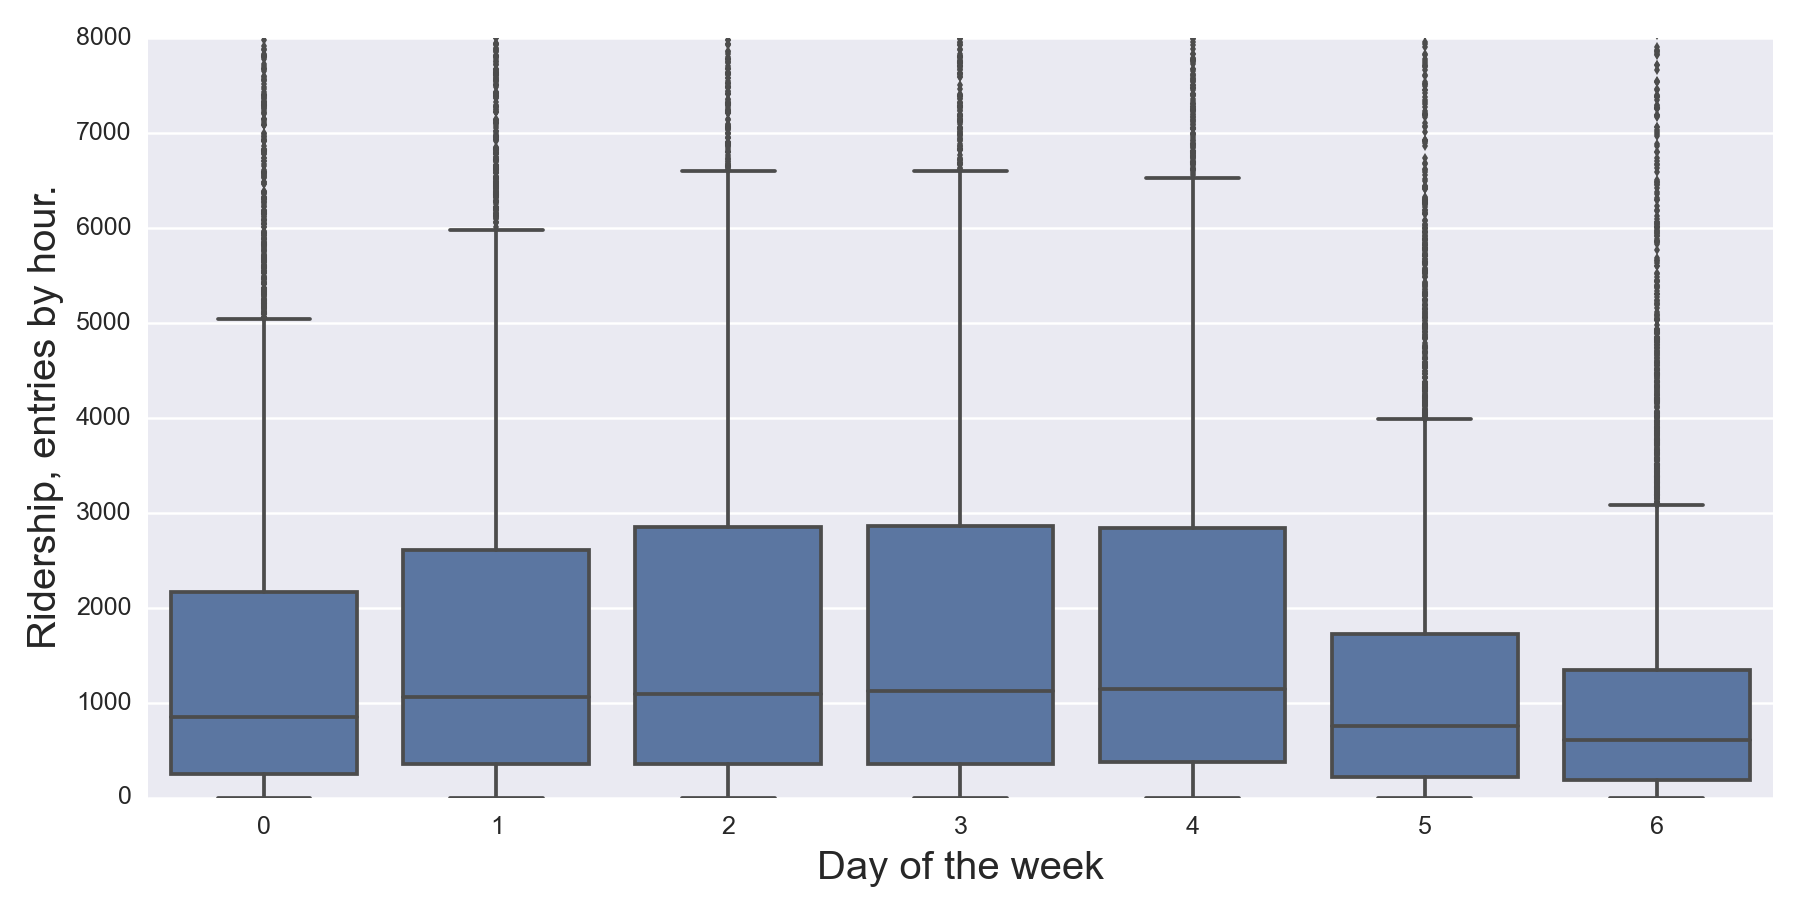
\includegraphics{day_rider.png}}
\caption{Ridership vs day of the week.}{\small 
This plot show the ridership distribution as boxplots for the 7 days of the
week (0 is Monday, 6 is Sunday). We can see that even when a relation
exist between day of the week and ridership, this relation doesn't look
linear, and thus we decided to use \code{weekday} instead.
}\label{section2:figure35}\end{figure}

Even when \code{UNIT} was not a numerical variable, we decided to use it given the
different ridership patterns for each turnstile location. When using it as
a dummy variable what we will be doing is adding or subtracting a constant
offset which is particular for each location. Will this be enough to model
the behaviors of different stations?

No further experiments where done to try other weather variables, since we were
mainly interested in the behavior of the system as a function of precipitations;
also, no other linear relationships were apparent from these variables, or
there was not enough data to sample the ridership under some conditions (e.g,
only 1 or 2 foggy days, no snow, etc.)

Finally, out from intuition we left out the variable \code{EXITSn}: besides having a
highly linearly correlated relation with the ridership variable, it is clear
that this variable is not completely independent from the number of entries to
subway. Furthermore, it won't be a nice predicting feature, since its value
will depend on the number of entries, and it should be treated as a observable
or predictable variable on itself.


\section{Results: coefficients and R Squared}
\label{section2:results-coefficients-and-r-squared}
\textbf{What are the coefficients (or weights) of the non-dummy features in your}
\textbf{linear regression model?}

\textbf{What is your model’s} \(R^2\) \textbf{(coefficients of determination) value?}

The coefficients found with the gradient descent and OLS algorithms were the
same in both cases, which was expected for a successful execution of the
gradient descent algorithm. The selected features were enough to obtain a
\(R^2 = 0.481\). More in depth details of the result can be seen in
{\hyperref[section2:table31]{\emph{Table 3.1}}}. Also, thanks to the statsmodels OLS implementation
we can report some of the coefficients obtained from the linear model fit,
using the predictor variables \code{hour}, \code{weekday}, \code{rain} and dummies from
\code{UNIT} ({\hyperref[section2:multreg-mod]{\emph{Eq. 3.1}}}), and their statistical significances
({\hyperref[section2:table32]{\emph{Table 3.2}}}).
\phantomsection\label{section2:table31}

\begin{threeparttable}
\capstart\caption{OLS Regression Results}

\begin{tabulary}{\linewidth}{|L|L|}
\hline
\textsf{\relax 
OLS Regression Results
} & \textsf{\relax }\\
\hline
Dep. Variable:        ENTRIESn\_hourly
 & 
R-squared:                       0.481
\\

Model:                            OLS
 & 
Adj. R-squared:                  0.478
\\

Method:                 Least Squares
 & 
F-statistic:                     163.1
\\

Date:                Wed, 07 Jan 2015
 & 
Prob (F-statistic):               0.00
\\

Time:                        14:12:52
 & 
Log-Likelihood:            -3.8397e+05
\\

No. Observations:               42267
 & 
AIC:                         7.684e+05
\\

Df Residuals:                   42027
 & 
BIC:                         7.705e+05
\\

Df Model:                         239
 & \\

Covariance Type:            nonrobust
 & \\
\hline\end{tabulary}

\end{threeparttable}

\phantomsection\label{section2:table32}

\begin{threeparttable}
\capstart\caption{Linear regression coefficients}

\begin{tabulary}{\linewidth}{|L|L|L|L|L|L|}
\hline
\textsf{\relax 
Predictor
} & \textsf{\relax 
coef
} & \textsf{\relax 
std err
} & \textsf{\relax 
t
} & \textsf{\relax 
P\textgreater{}\textbar{}t\textbar{}
} & \textsf{\relax 
{[}95\% Conf. Int.{]}
}\\
\hline
\textbf{Intercept}
 & 
-1750.5171
 & 
166.661
 & 
-10.503
 & 
0.000
 & 
-2077.175 -1423.859
\\

C(UNIT){[}T.R004{]}
 & 
334.1581
 & 
231.108
 & 
1.446
 & 
0.148
 & 
-118.819   787.135
\\

C(UNIT){[}T.R005{]}
 & 
335.0522
 & 
232.095
 & 
1.444
 & 
0.149
 & 
-119.859   789.963
\\

C(UNIT){[}T.R006{]}
 & 
451.3319
 & 
229.532
 & 
1.966
 & 
0.049
 & 
1.445   901.218
\\

C(UNIT){[}T.R007{]}
 & 
164.5844
 & 
232.767
 & 
0.707
 & 
0.480
 & 
-291.644   620.812
\\

...
 & 
...
 & 
...
 & 
...
 & 
...
 & 
...       ...
\\

\textbf{hour}
 & 
124.0989
 & 
1.500
 & 
82.741
 & 
0.000
 & 
121.159   127.039
\\

\textbf{weekday}
 & 
980.9091
 & 
23.243
 & 
42.203
 & 
0.000
 & 
935.353  1026.465
\\

\textbf{rain}
 & 
36.3145
 & 
25.167
 & 
1.443
 & 
0.149
 & 
-13.013    85.642
\\
\hline\end{tabulary}

\end{threeparttable}



\section{Interpretation and limits}
\label{section2:interpretation-and-limits}
\textbf{What does this} \(R^2\) \textbf{value mean for the goodness of fit for your regression}
\textbf{model? Do you think this linear model to predict ridership is appropriate for}
\textbf{this dataset, given this} \(R^2\) \textbf{value?}

Even when a relatively high \(R^2\) was achieved by the use of a multiple
linear regression model, a successful model should also comply with several
assumptions, which can be checked by analysing the residuals {\hyperref[overview:diez2012]{{[}Diez2012{]}}}.
\begin{enumerate}
\item {} 
\textbf{Are the residuals for the model nearly normal?}:
{\hyperref[section2:figure36]{\emph{figure 3.6 top rows}}}, shows that the residuals obtained do
not seem to follow a normal distribution. Even when the peak of the residuals
tend to be zero, the wings do not follow a Gaussian distribution, as is more
easily seen on the top left plot. Most probably, we have a big number of
outliers.

\end{enumerate}
\begin{figure}[htbp]
\centering
\capstart

\scalebox{1.000000}{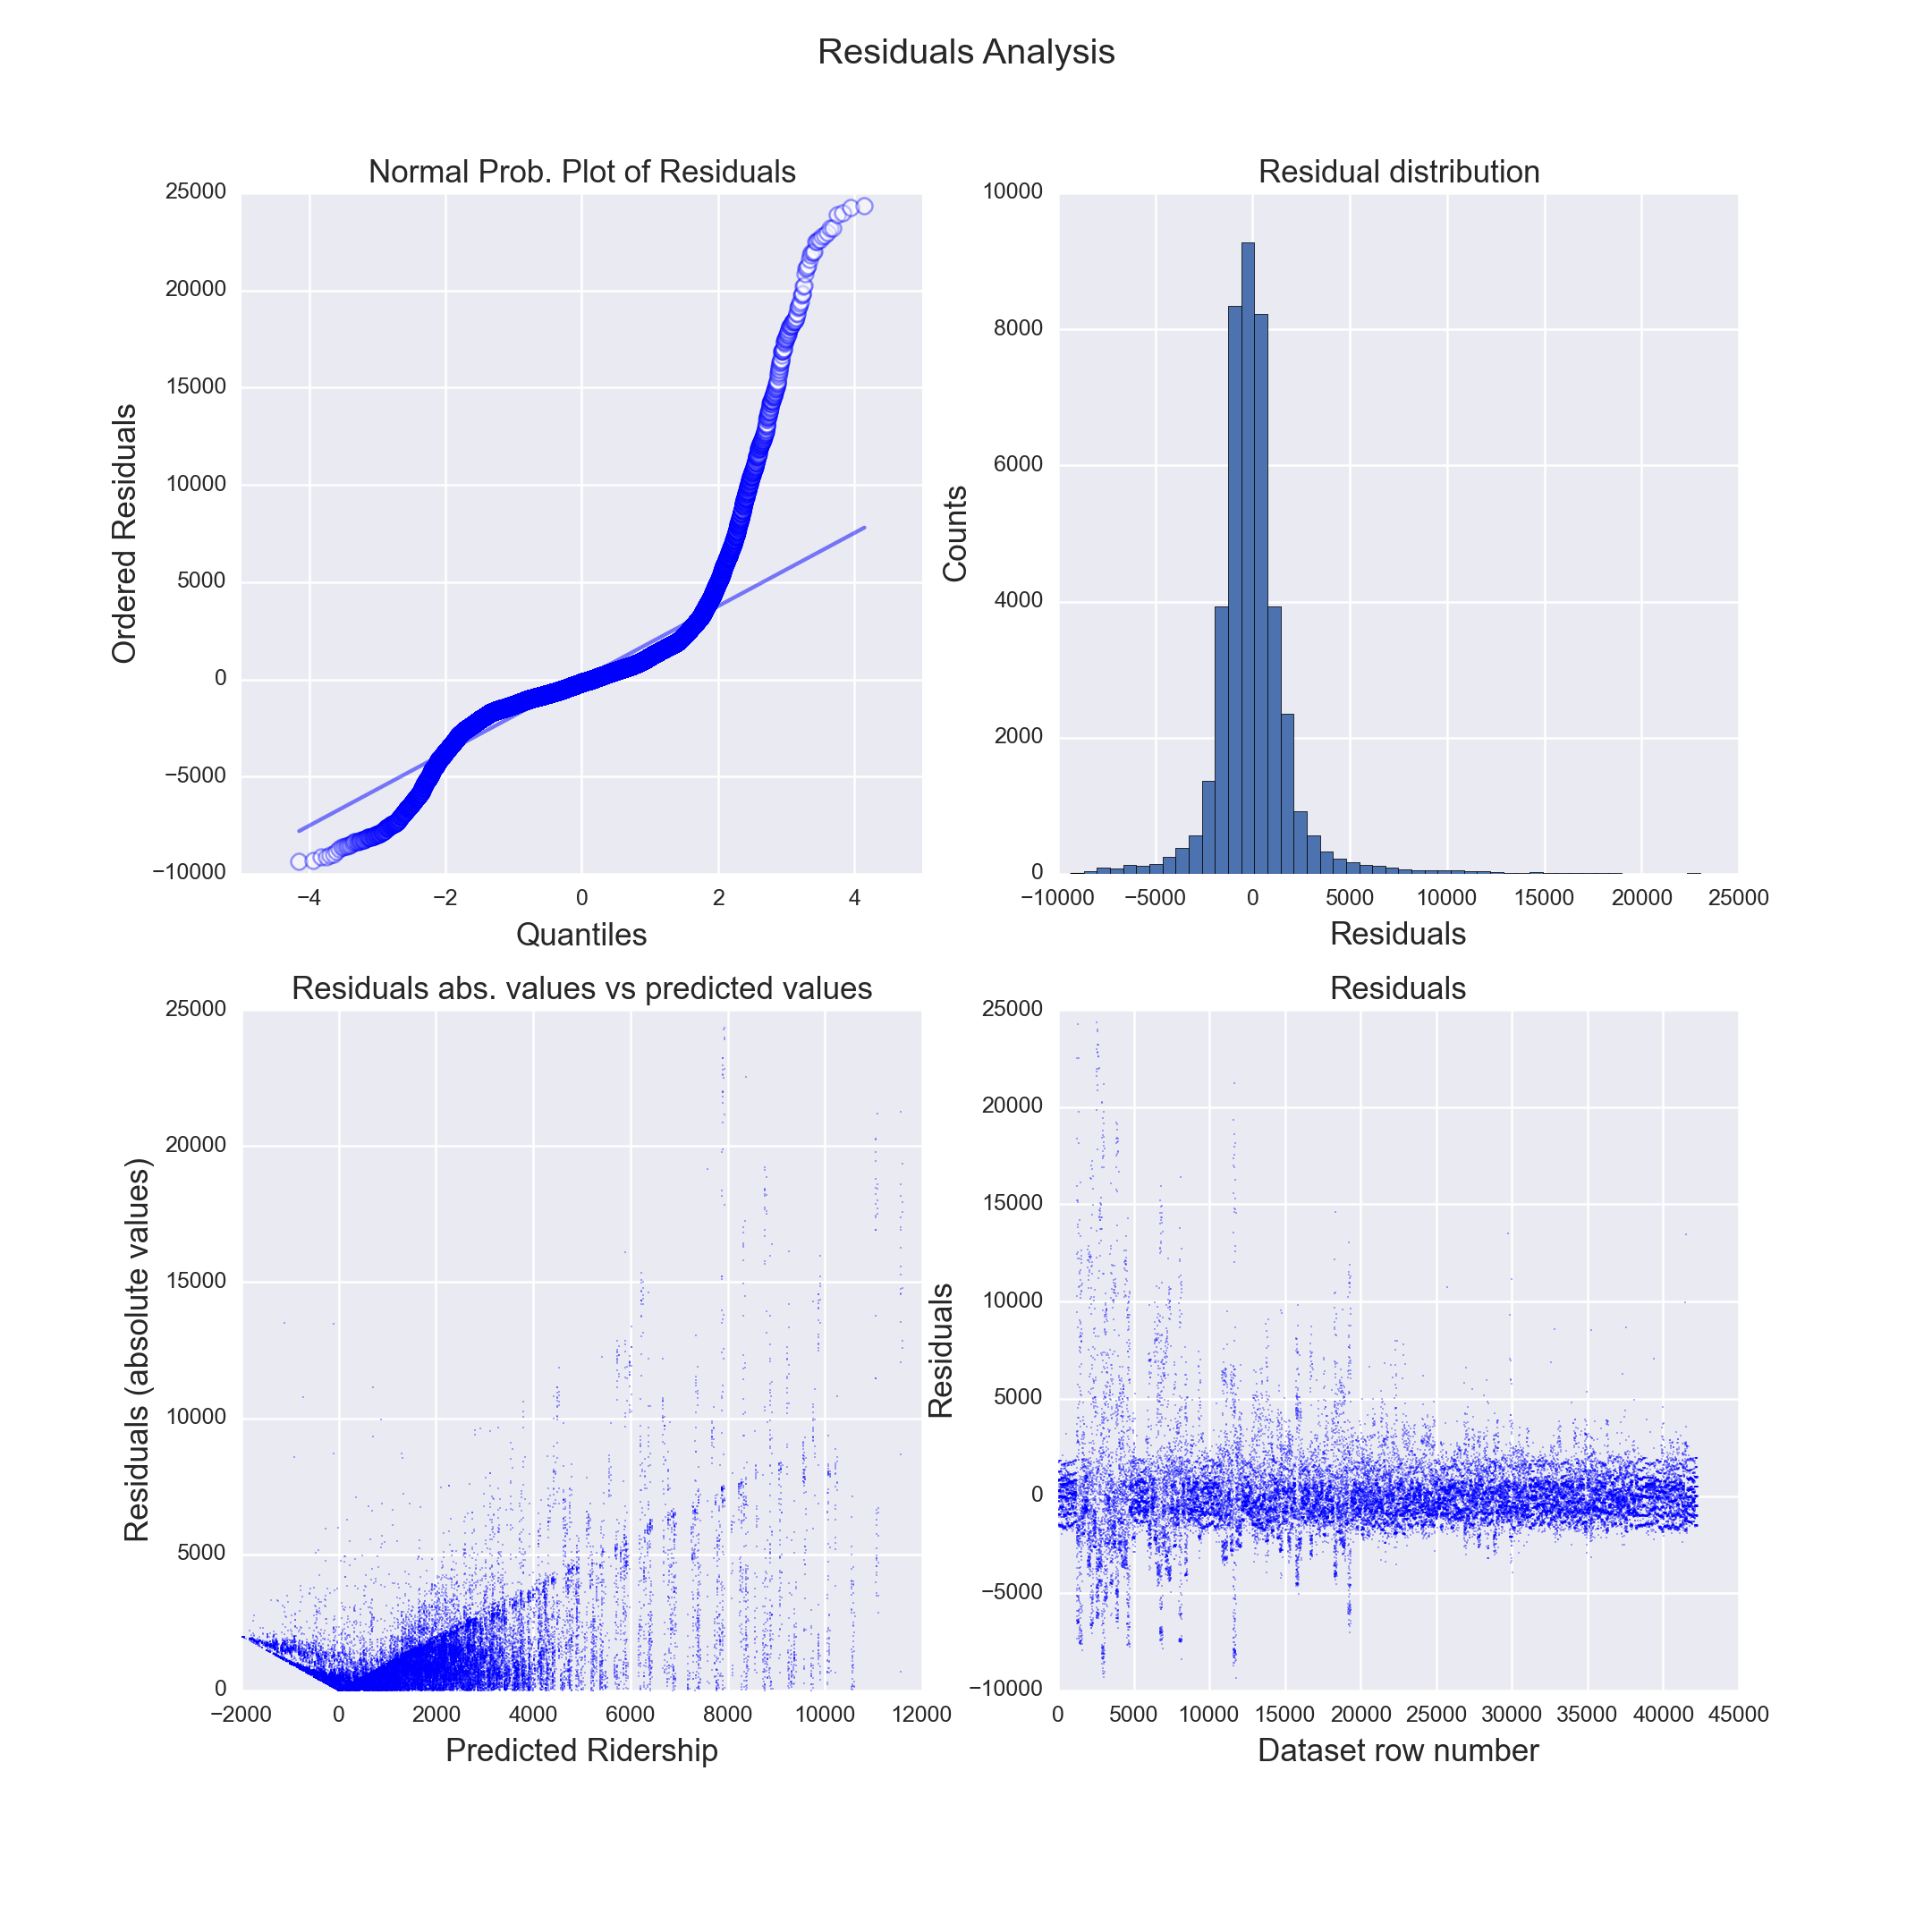
\includegraphics{residuals_an.png}}
\caption{Residuals analysis plots for the linear regression model (improved dataset).}{\small 
\emph{Top left:} normal probability plot of the residuals and \emph{top right:} residuals
distribution. It is clear that residuals do not adjust well to a simple normal
probability distribution. \emph{Bottom left} shows the residuals versus the
predicted ridership, and \emph{bottom right} just the residuals following the order
on which the observed values were found on the improved dataset.
}\label{section2:figure36}\end{figure}
\begin{enumerate}
\setcounter{enumi}{1}
\item {} 
\textbf{Is the variability of the residuals nearly constant?}: the variance of the
residuals can be checked on the bottom left plot of {\hyperref[section2:figure36]{\emph{figure 3.6}}},
where the residuals vs predicted values are plotted. The figure doesn't show
a constant variance along the x axis, with a lot of features that might be
related to a poorly fit.

\item {} 
\textbf{Are the residuals independent?}: a plot of the residuals in the order of the
data collected in the original data frame should show no relation between
close neighbours. Our data frame mix data from several turnstiles, but it is
ordered in such way that all data from the turnstiles can be found on sequenced
blocks, where the data is again ordered by date and time. From the bottom right
plot on {\hyperref[section2:figure36]{\emph{figure 3.6}}} it seems that the residuals do not look
independent between different turnstiles.

\item {} 
\textbf{Is each variable linearly related to the outcome?}: we can check the linearity
from the figures presented in section 3.2; also the reader can check some
other figures withing the ipython notebook associated to this project. It has
been already established that there is a linear relation between ridership and
the variables \code{weekday} and \code{rain}; however there is a poor relation with
the \code{hour} variable ({\hyperref[section2:figure37]{\emph{figure 3.7}}}). However, there are some
issues raised given the way the \code{UNIT} variable was included in the model,
and that can be seen in the plots shown in {\hyperref[section2:figure37]{\emph{figure 3.8}}}
and {\hyperref[section2:figure39]{\emph{figure 3.9}}}.

\end{enumerate}
\begin{figure}[htbp]
\centering
\capstart

\scalebox{0.900000}{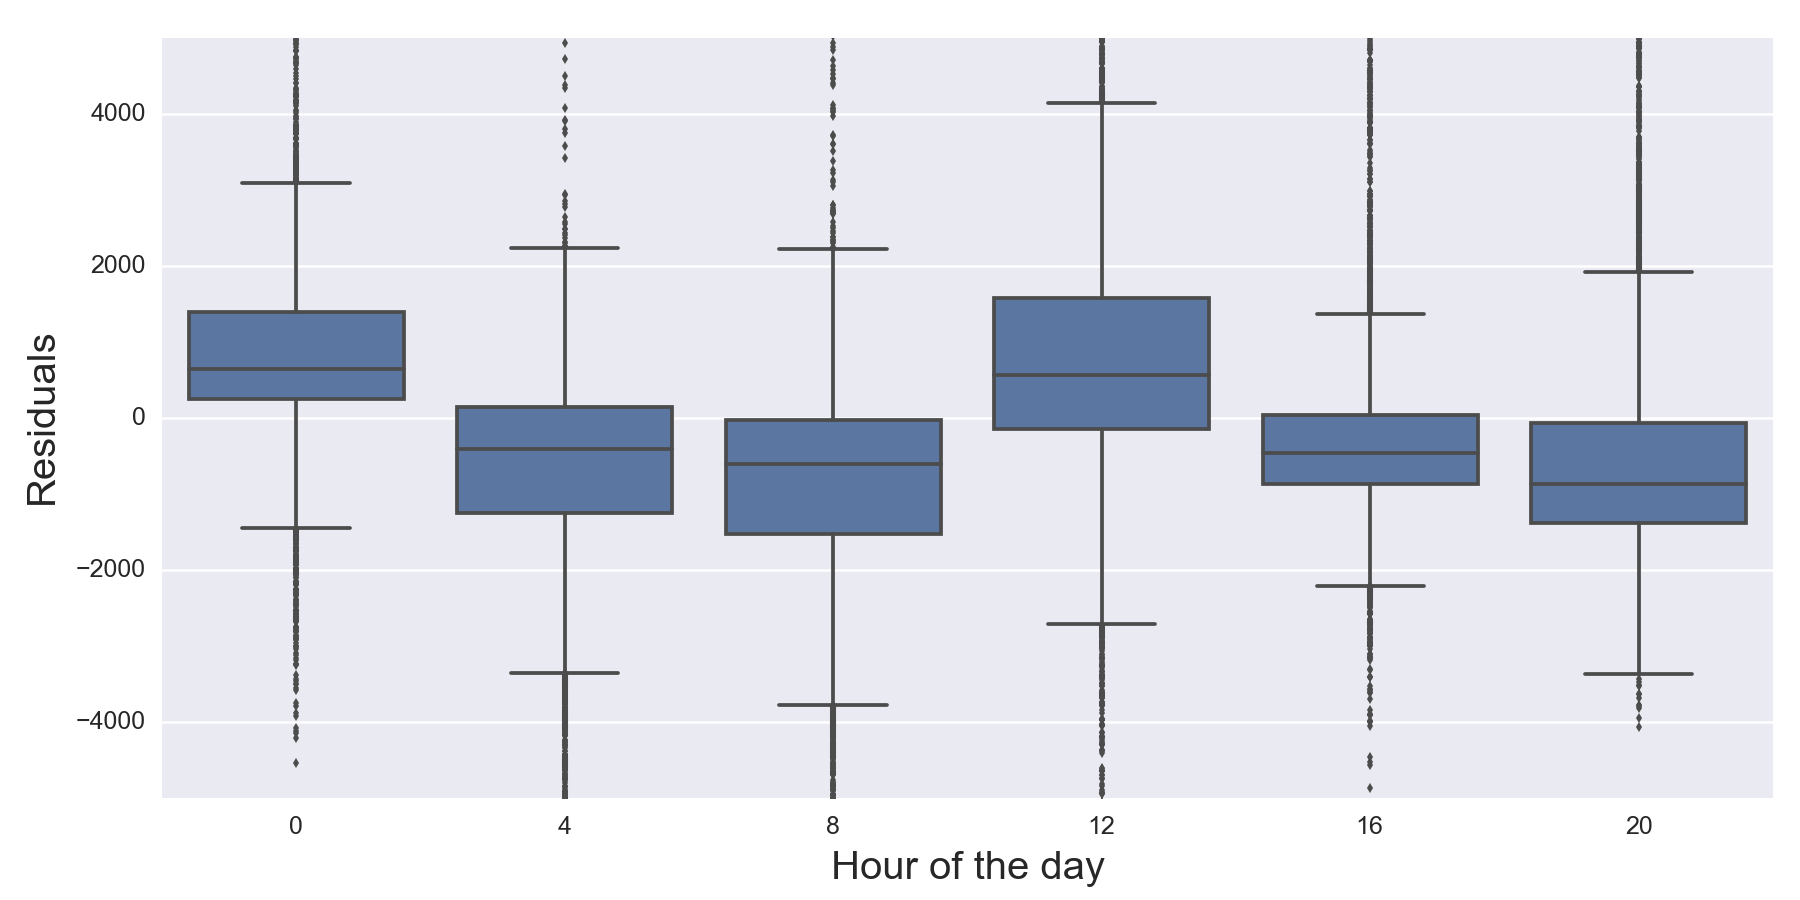
\includegraphics{hour_residuals.png}}
\caption{Residuals (as boxplots) vs hour of the day.}\label{section2:figure37}\end{figure}
\begin{figure}[htbp]
\centering
\capstart

\scalebox{0.900000}{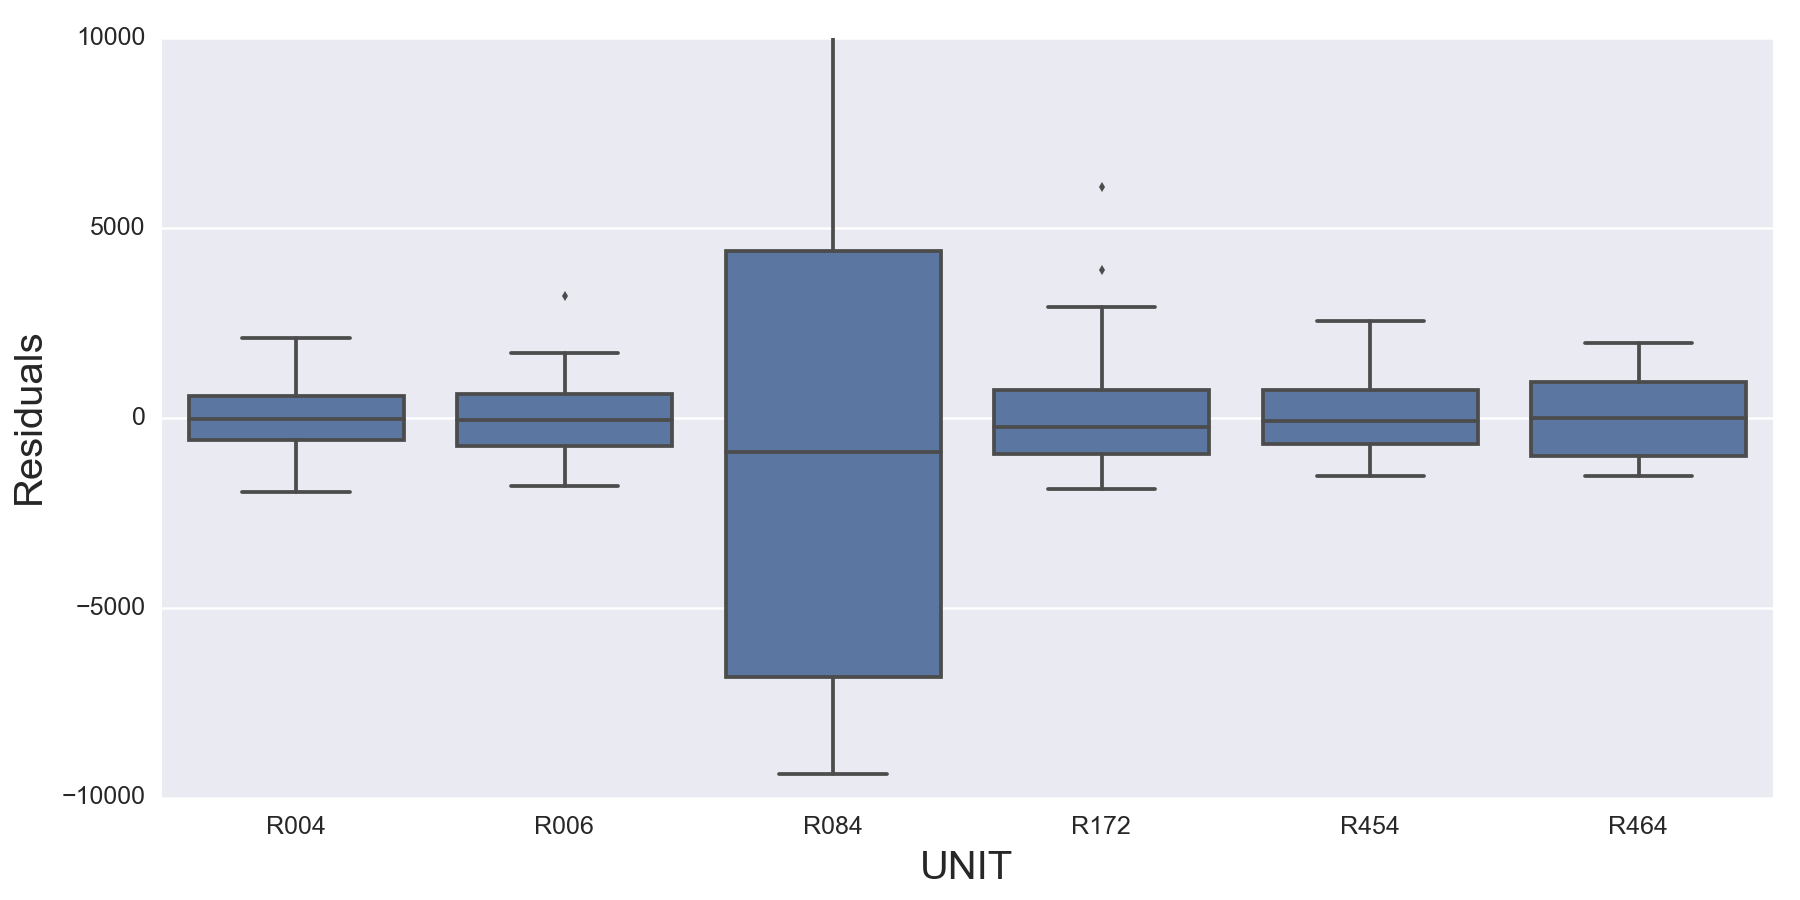
\includegraphics{turns_residuals.png}}
\caption{Residuals (as boxplots) for different turnstiles.}\label{section2:figure38}\end{figure}
\begin{figure}[htbp]
\centering
\capstart

\scalebox{0.900000}{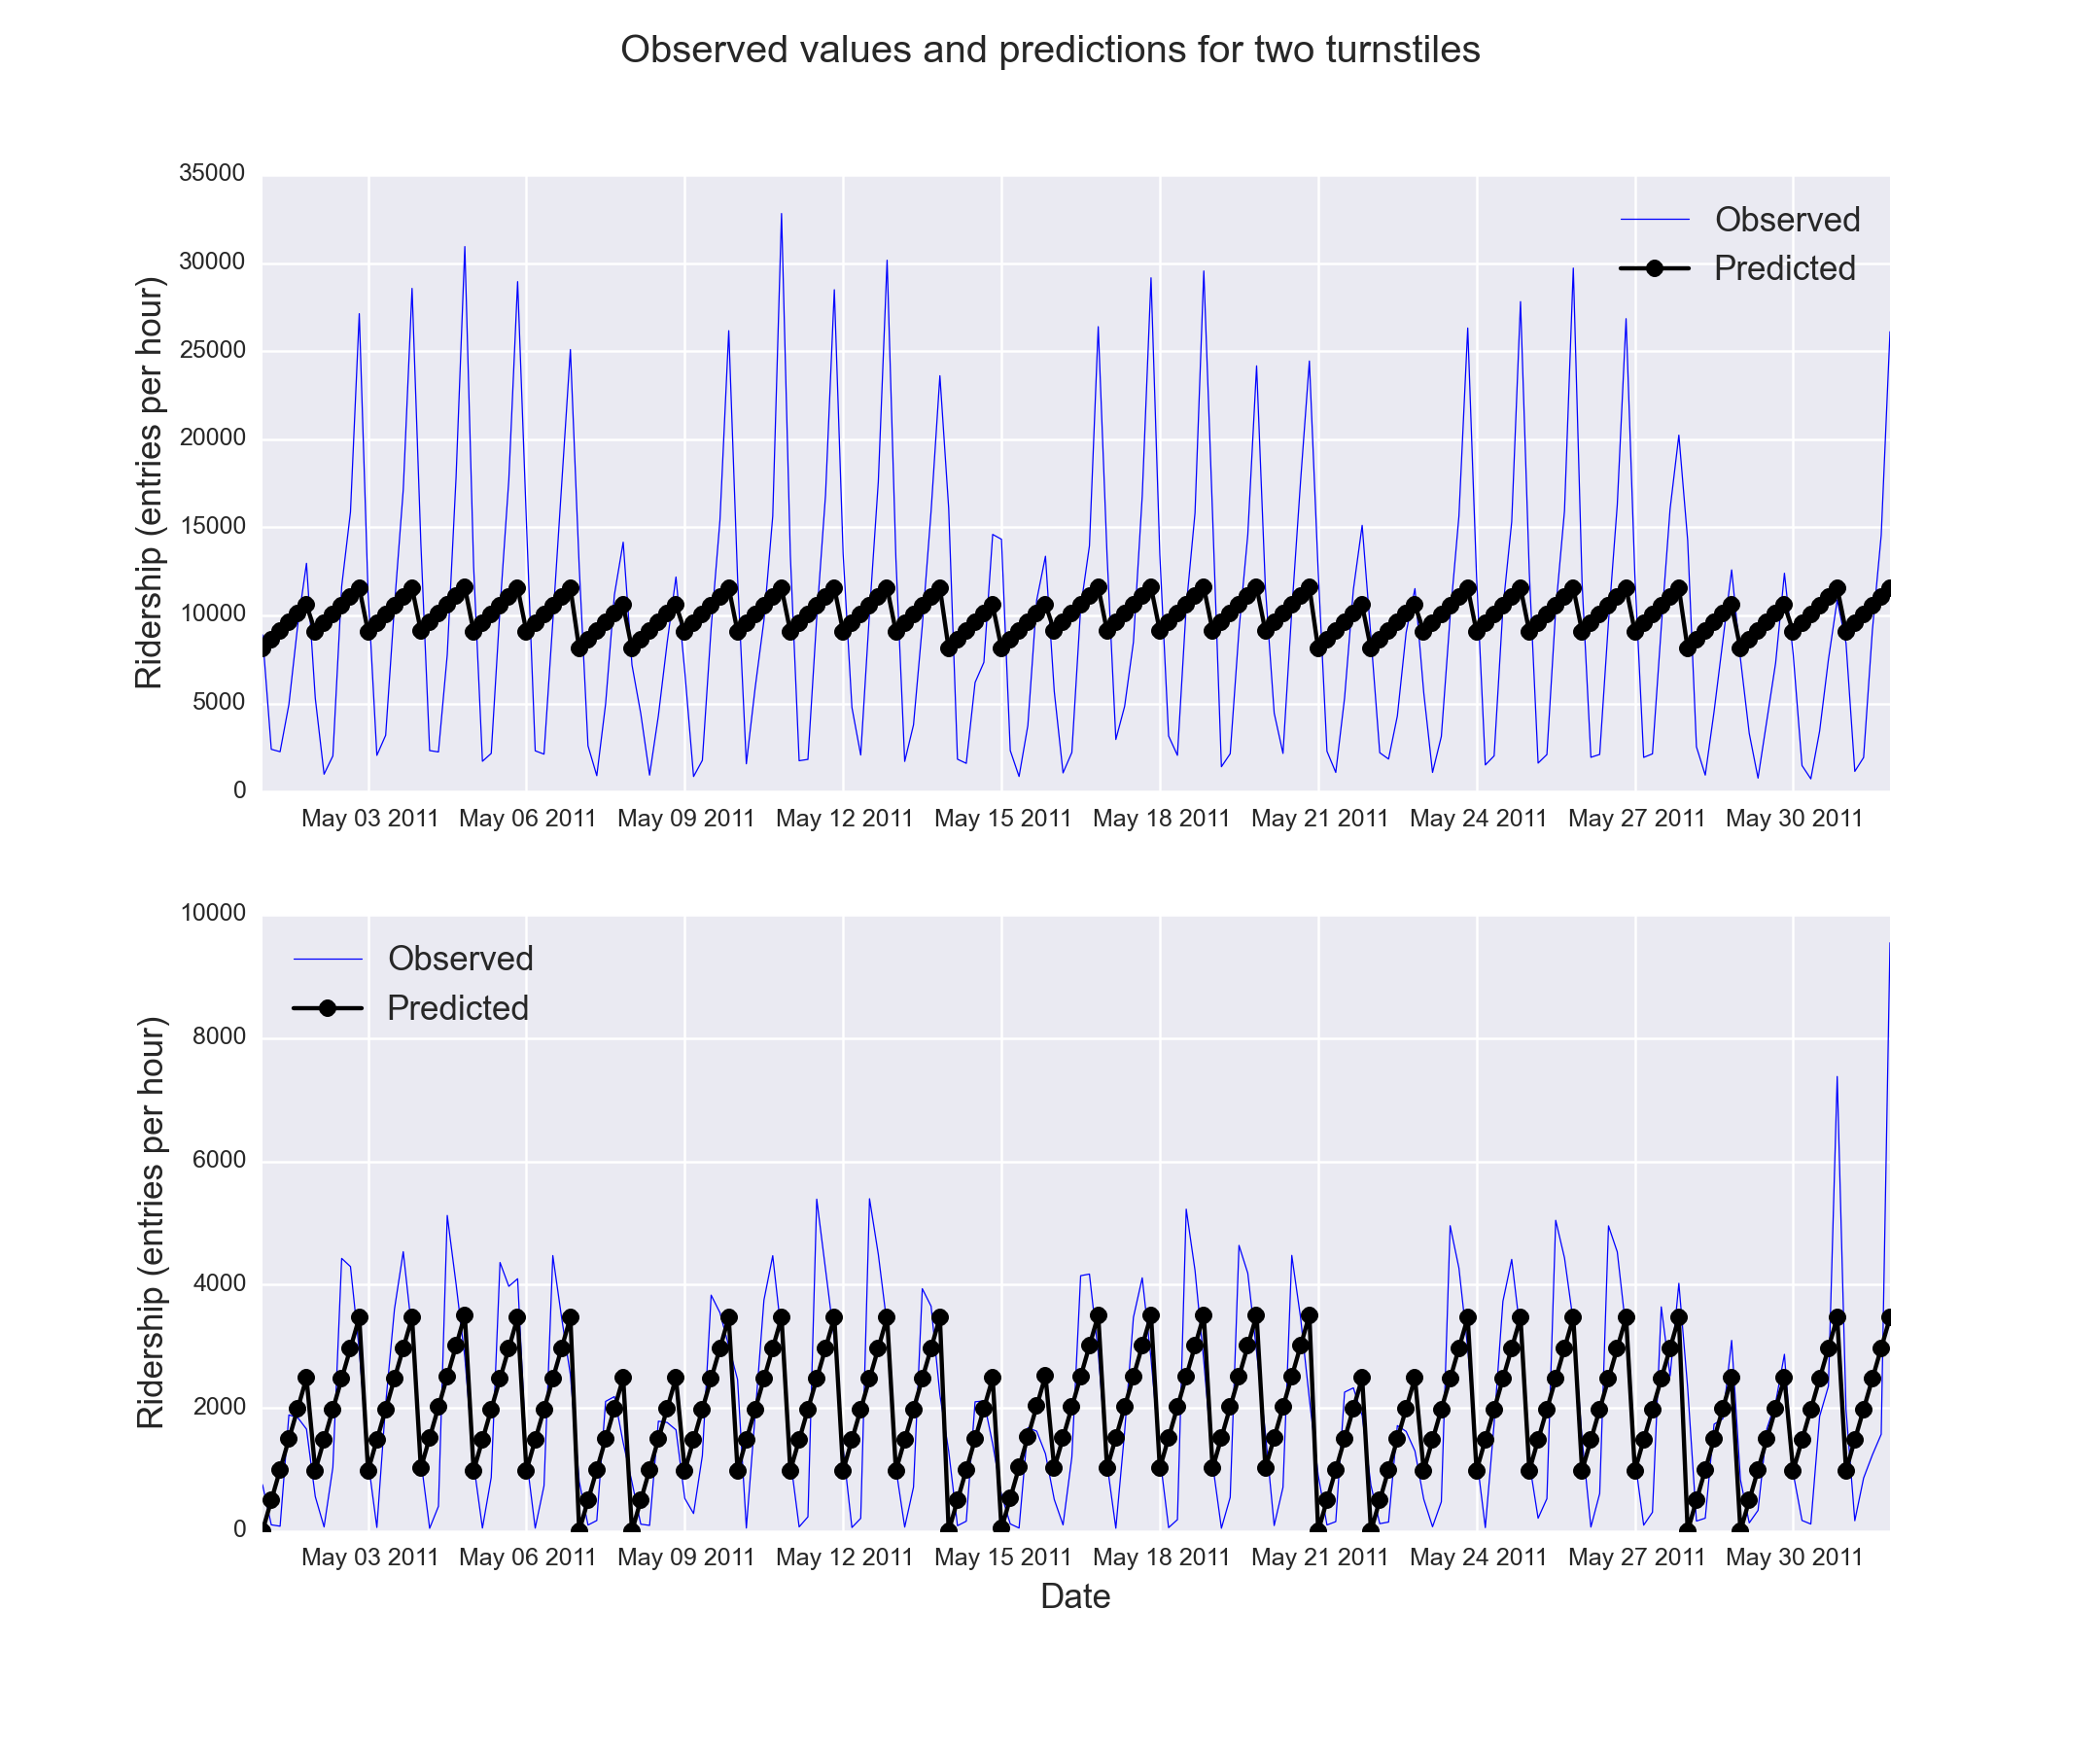
\includegraphics{turns_pred.png}}
\caption{Observed and predicted ridership values for three different turnstiles.}{\small 
The turnstiles used were R084, R172 and R338, one at downtown and the other
two at the periphery. The predicted values come from the linear regression
model applied in previous section. Note how besides the middle panel, the
model predictions do not follow well the observed ridership for stations with
too much traffic or low traffic. Also, because of the way the \code{UNIT} dummy
variables are used, we can see that just adding a constant is not enough to
scale the ridership for individual locations.
}\label{section2:figure39}\end{figure}

Besides the mild coefficient of determination it seems that many of the
assumptions are not met by our data to successfully apply a multiple regression
model to it. The residuals analysis are very good indicators of the behaviors of
the ridership that the model can't explain, mainly because it was a very rough
assumption to use \code{hour} as it is clearly not well modeled by the linear
regression ({\hyperref[section2:figure37]{\emph{figure 3.7}}}). {\hyperref[section2:figure39]{\emph{Figure 3.9}}} is also
a nice diagnosis tool to show that using the turnstiles names as dummy variables
can help to improve the fit to the model, but is not enough. From the figure we
can see again that the ridership varies from location to location, with peaks
and valley hours happening at different times of the day for different
turnstiles. Our model only corrects each turnstile by adding or subtracting a
constant to each turnstile, which is not enough to model the ridership of the
different locations. We also found that given the negative value of the
intercept coefficient and small values for some turnstile coefficients we have
several ridership predictions that are negative: this is meaningless for our
problem, since is doesn't make sense a negative ridership.

Finally, it is interesting to independently check that even when the \code{rain}
variable can be fit by a linear model, it significance is very low as can be
seen by the low p-value of the coefficient: 0.15. In fact, removing \code{rain} as
predictor feature only reduce the \(R^2\) by less than 0.0001, and the
reported coefficient of determination is still 0.481.


\subsection{Aggregated dataset and polynomial features}
\label{section2:aggregated-dataset-and-polynomial-features}
We will now take advantage to the extra wrangling done with the improved data
set in the previous chapter, and we will use the smoothed dataset that we
created: \textbf{nycsubway\_weather}. This data set was created by aggregating the
ridership for each time stamp by adding all the ridership of the individual
turnstiles, so we have a dataset that reports the ridership of the NYC subway as
a whole. The columns of this dataset are:
\begin{itemize}
\item {} 
ENTRIESn\_hourly: the total ridership as entries per hour for the whole NYC
subway system

\item {} 
dateTime: \code{datetime} variable, is the date and time for each observed value.

\item {} 
hour: integer value, is the hour of the day for each reported value. It has a
24 hour format.

\item {} 
day\_week: integer value, is the day of the week for the observation (0 for
Monday, 6 for Sunday)

\item {} 
weekday: indicator variable, 1 for a weekday, 0 for a weekend day.

\item {} 
holiday: categorical variable, 1 for days that are holidays.

\item {} 
rain\_hour: indicator variable, it reports whether at any location within the
NYC Subway system was raining at the particular time

\item {} 
rain\_day: indicator variable, it reports whether at any location in the NYC
Subway system there wa any precipitation (rain) for the particular day of the
reported value.

\end{itemize}

After some tries with multiple regression models, using the OLS statsmodels
implementation, we were able to raise the \(R^2\) value to 0.563 using this
new dataset and three predicting variables: \code{hour}, \code{weekday} and \code{holiday}.
Neither \code{rain\_day} nor \code{rain\_hour} improved the coefficient of determination
noticeably, with p-values higher than 0.61. Even with the smoothing achieved
by the removal of individual turnstiles we were able to see the same kinds of
problems as described previously, being the most important factor the
nonlinearity of the relation between the hour of the day and ridership, plus the
difference in this relation for different days of the week: having a constant
added (or subtracted) given the type of day (weekday or day off) is not enough
to account for the variations seen between days.
{\hyperref[section2:figure310]{\emph{Figure 3.10}}} shows a plot with the observed and predicted
values, which further explains the shortcoming of using a linear model with our
data. The reader can also check the ipython notebook associated with this
project to look for the residuals analysis.
\begin{figure}[htbp]
\centering
\capstart

\scalebox{0.900000}{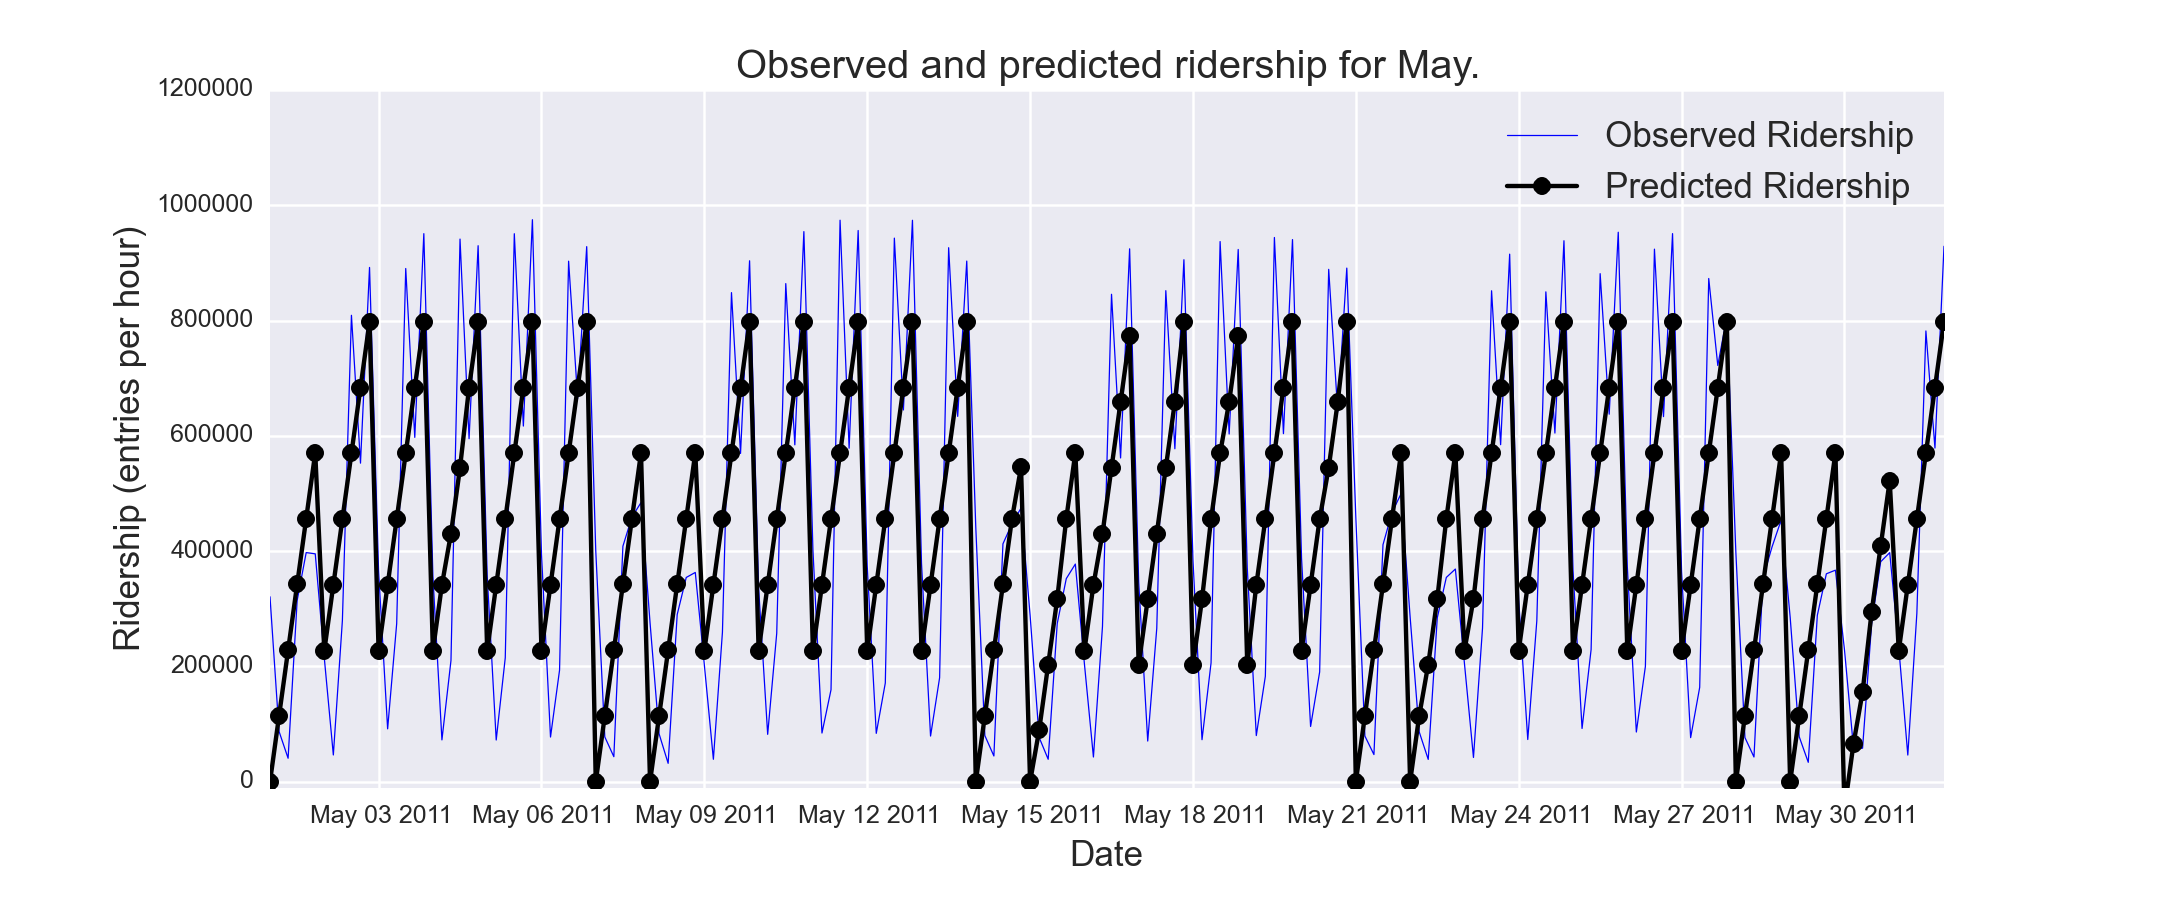
\includegraphics{subway_may.png}}
\caption{Observed and predicted ridership values for the NYC Subway, month of May.}{\small 
Even when we have eliminated the complexities by taking the whole NYC Subway
as a whole and increased the percentage of the ridership behavior for May
2011 that is explained but the used linear model, is still apparent the
problems produced by the lack of linearity of \code{hour} vs ridership, and the
changes in ridership behavior for different days of the week.
}\label{section2:figure310}\end{figure}

Because of these reasons we decide to try a different method. This method is still
an algorithm that uses the linear regression tools, but the predictors are now
converted into \emph{polynomial features} {\hyperref[overview:glmscikit]{{[}glmscikit{]}}}. The problem can be resolved with
a linear regression by taking advantage of the linearity of the coefficients in
the system of equations needed to solve the problem of finding these coefficients.
The function used to convert our selected predictors, that for this optional exercise
will be \code{hour}, \code{day\_week}, \code{holiday} and \code{rain\_hour}, was the library
\code{PolynomialFeatures} from the scikit-learn libraries for machine learning with
python. We won't enter into the details of this method, since it goes beyond
the goal of this project, but it suffice to say here that the new model is now
a polynomial of degree 5 (that was our selection), were the predictors also interact
with each other. So, if \(x_1 = \rm{hour}\), \(x_2 = \rm{day_week}\),
\(x_3 = \rm{holiday}\) and \(x_3 = \rm{rain\_hour}\), the model we are
trying to use to explain our data is going to be of the form:
\begin{gather}
\begin{split}\hat{y} = \theta_0 + \theta_1 x_1 + \theta_2 x_1^2 + ... + \theta_5 x_1^5 +
\theta_6 x_2 +...+ \theta_n x_1 x_2 + \theta_{n+1} x_1 x_3 + ...\end{split}\notag
\end{gather}
Also, we mentioned that we used a Ridge regression algorithm, that was suggested
by the scikit-learn documentation as a more robust method to find the coefficients
in a model like the one we are trying to use.

The main idea was to try to overcome the limitation given for the non-linearity
of the hourly and daily ridership in our NYC subways system set. The improvement
was amazing, by reaching a \(R^2 = 0.968\), and the reader can check the
residual analysis plots in {\hyperref[section2:figure311]{\emph{Figure 3.11}}}.
\begin{figure}[htbp]
\centering
\capstart

\scalebox{1.000000}{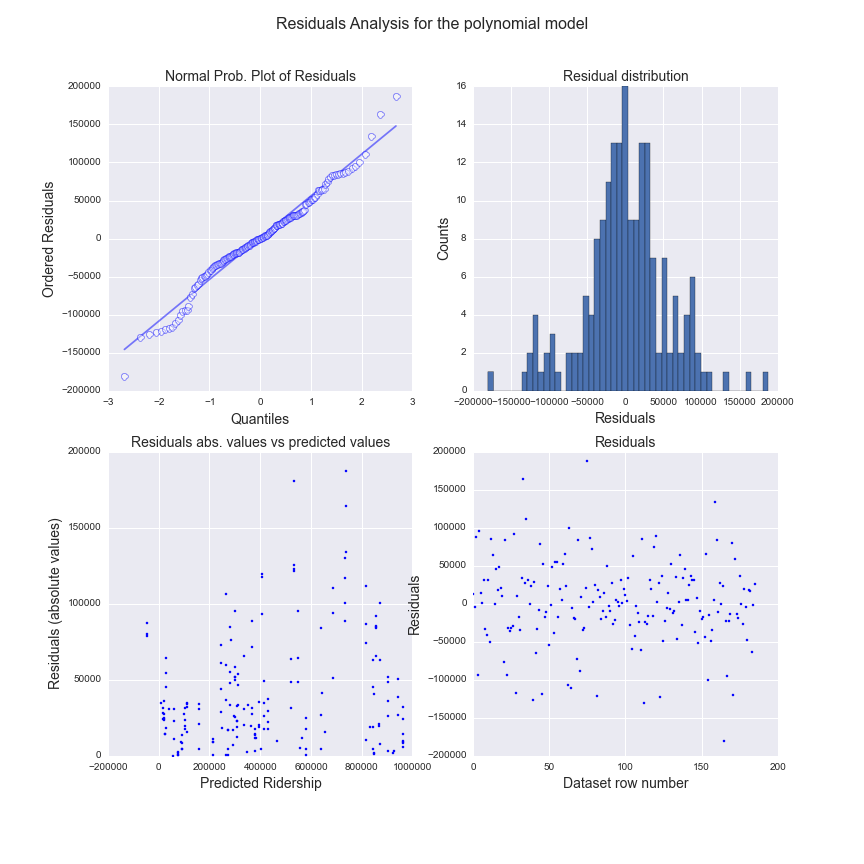
\includegraphics{poly_resid.png}}
\caption{Residuals analysis plots for the polynomial model (nycsubway\_weather dataset).}{\small 
\emph{Top left:} normal probability plot of the residuals and \emph{top right:} residuals
distribution. The residuals are distributed now following more closely the shape
of a Gaussian, and less outliers are visible; \emph{Bottom left} shows the residuals
versus the predicted ridership, and \emph{bottom right} just the residuals following
the order on which the observed values are reported.
}\label{section2:figure311}\end{figure}

Even when (a) the residual distribution is now closer to a normal distribution,
(b) the variance seems to be more constant and (c) the residuals seem
independent, we must draw the attention to the reader to the fact that this
model, while an improvement, still have shortcomings, that can be seen in
{\hyperref[section2:figure312]{\emph{Figure 3.12}}}. While the hourly and daily ridership are now
modeled with higher precision we have to be aware of the overfitting our model
is suffering of, explained by the large number of coefficients to be found
(126 coefficients). However, it is clear that a much better work can be done
with more complex machine learning algorithms, and the idea was just to show
that with the data we have we should be able to predict ridership with much more
accuracy than the linear regression is capable of.
\begin{figure}[htbp]
\centering
\capstart

\scalebox{1.000000}{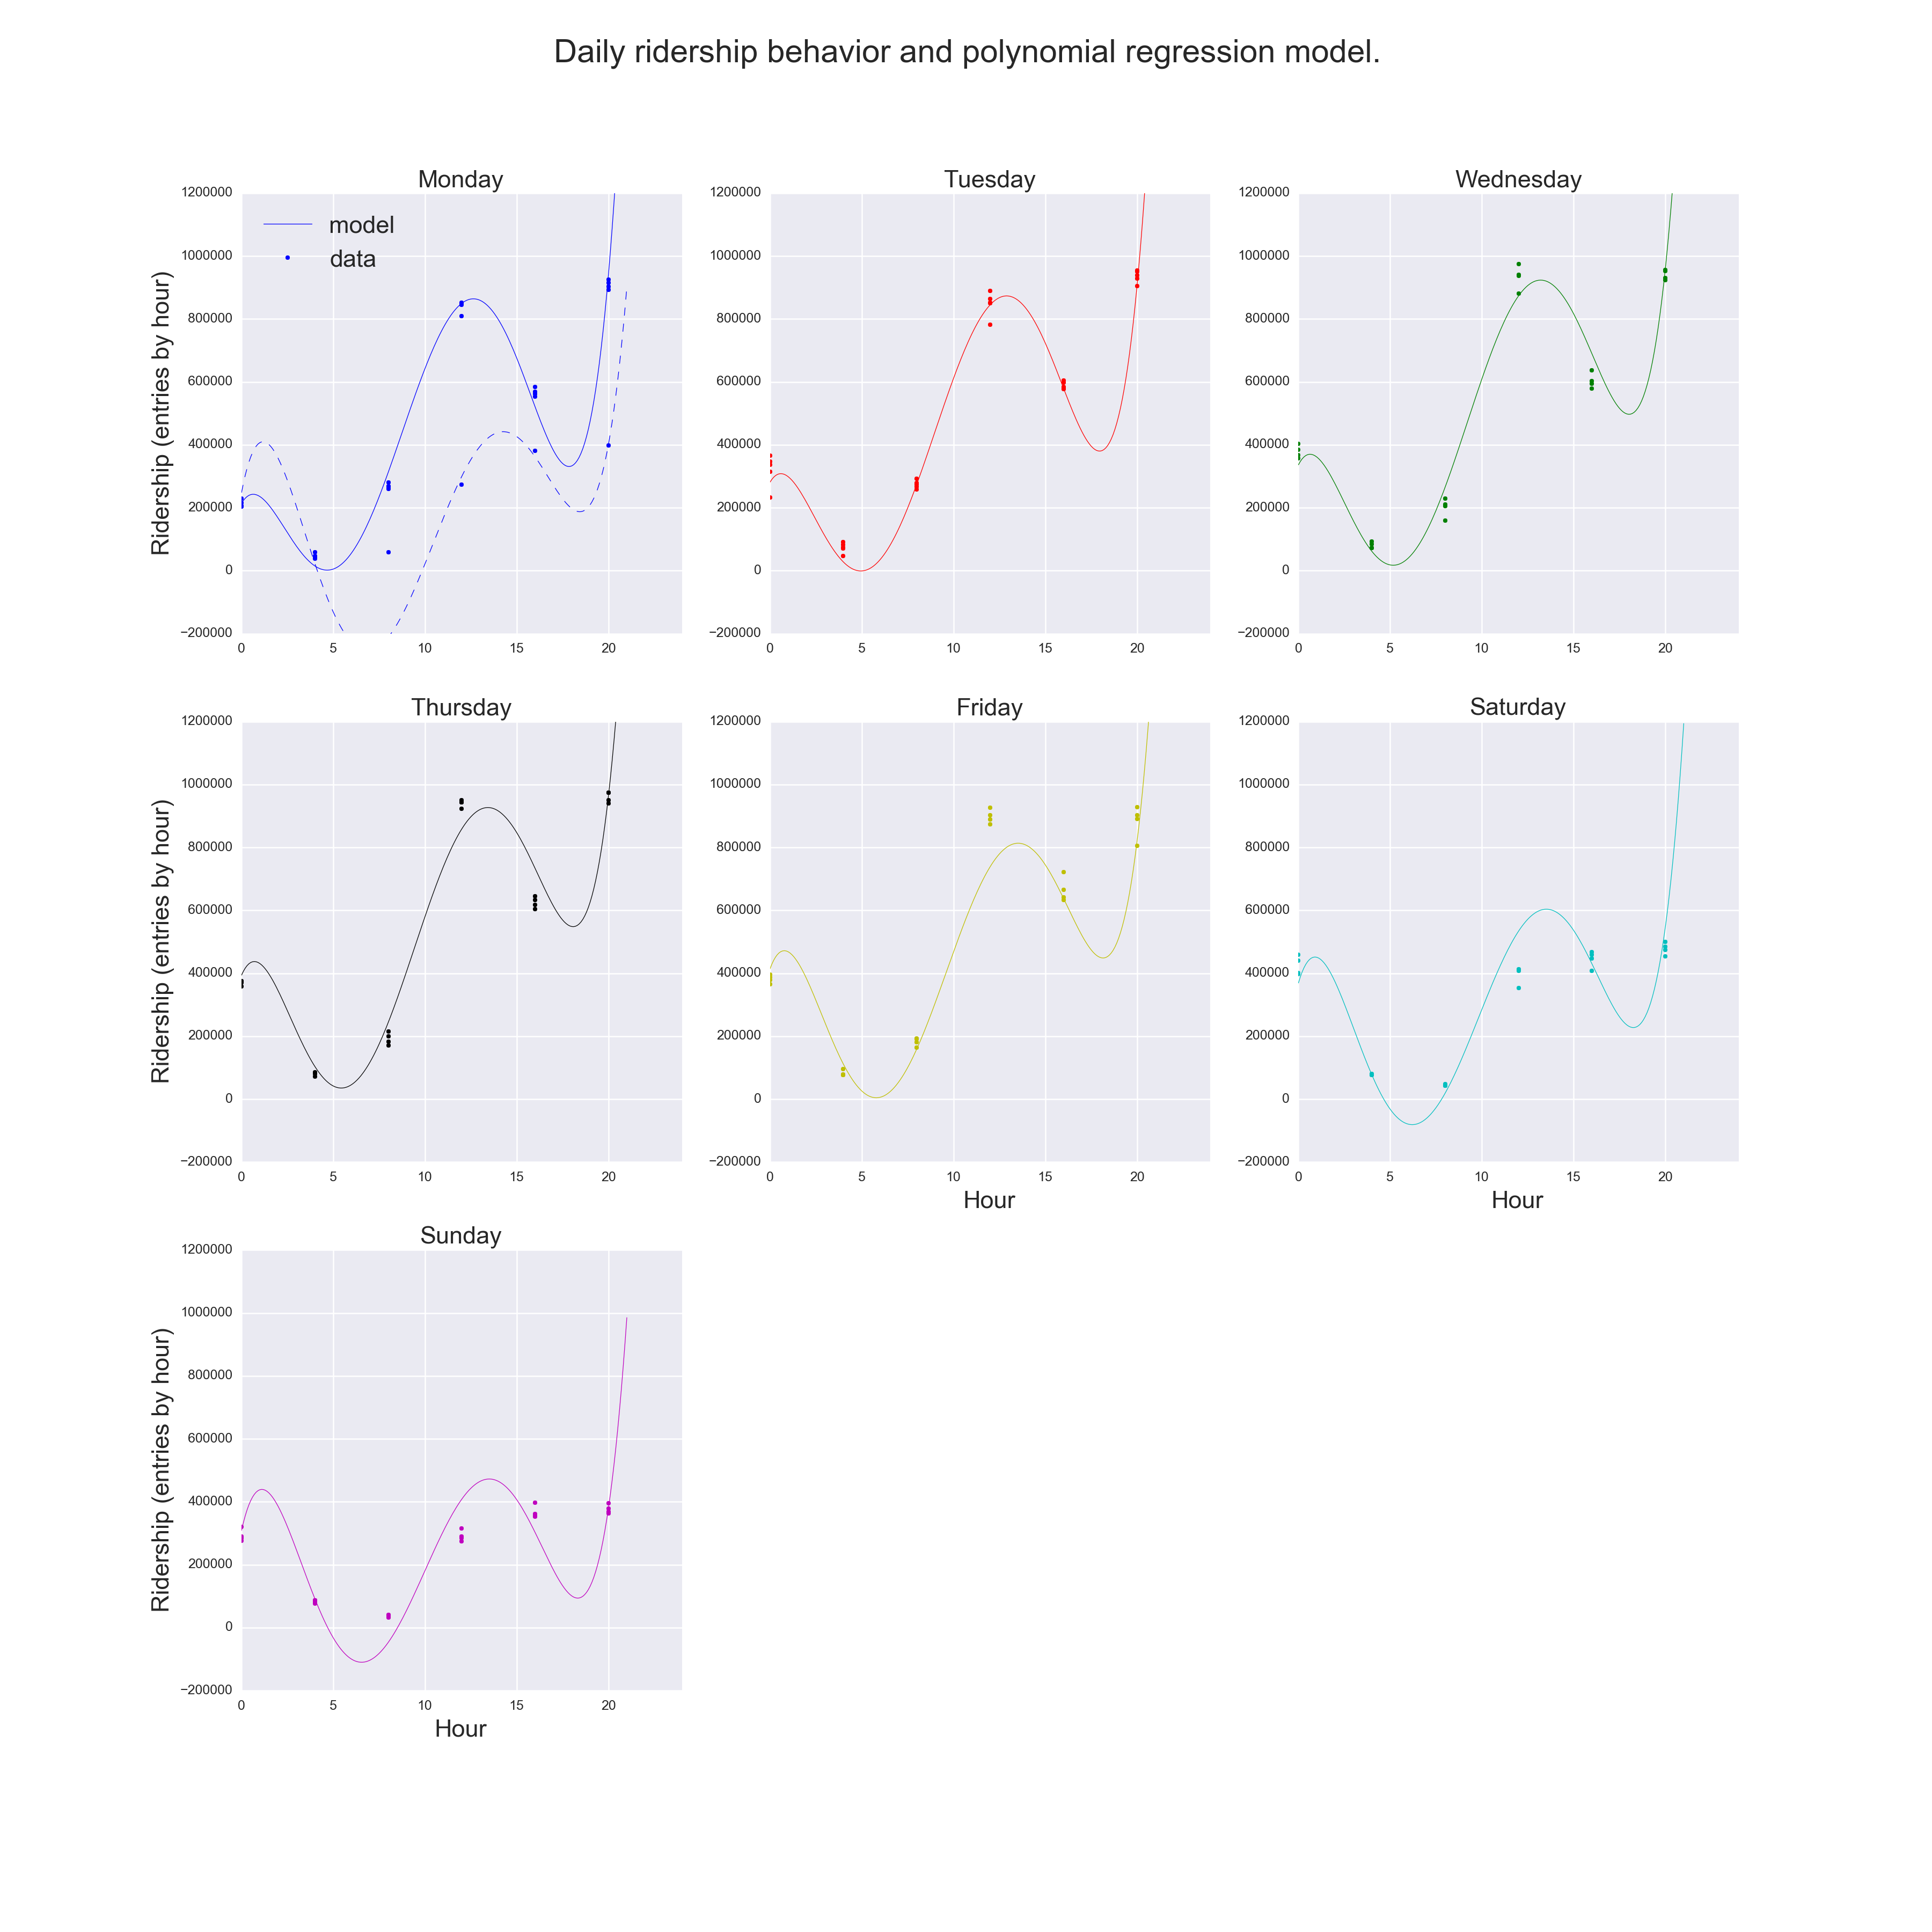
\includegraphics{polyfit.png}}
\caption{Observed and predicted ridership values for days of the week as a function of
hour.}\label{section2:figure312}\end{figure}


\chapter{Visualization}
\label{section3:visualization}\label{section3::doc}

\section{Ridership distribution with weather}
\label{section3:ridership-distribution-with-weather}
\textbf{One visualization should contain two histograms: one of  ENTRIESn\_hourly for}
\textbf{rainy days and one of ENTRIESn\_hourly for non-rainy days.}

The figure comparing the ridership distributions for rainy and non-rainy days
has been already presented in the Chapter 2. Here ({\hyperref[section3:figure42]{\emph{figure 4.1}}})
we show the same figure, but this time we want to show the different samples sizes
by not normalizing the data.
\begin{figure}[htbp]
\centering
\capstart

\scalebox{0.800000}{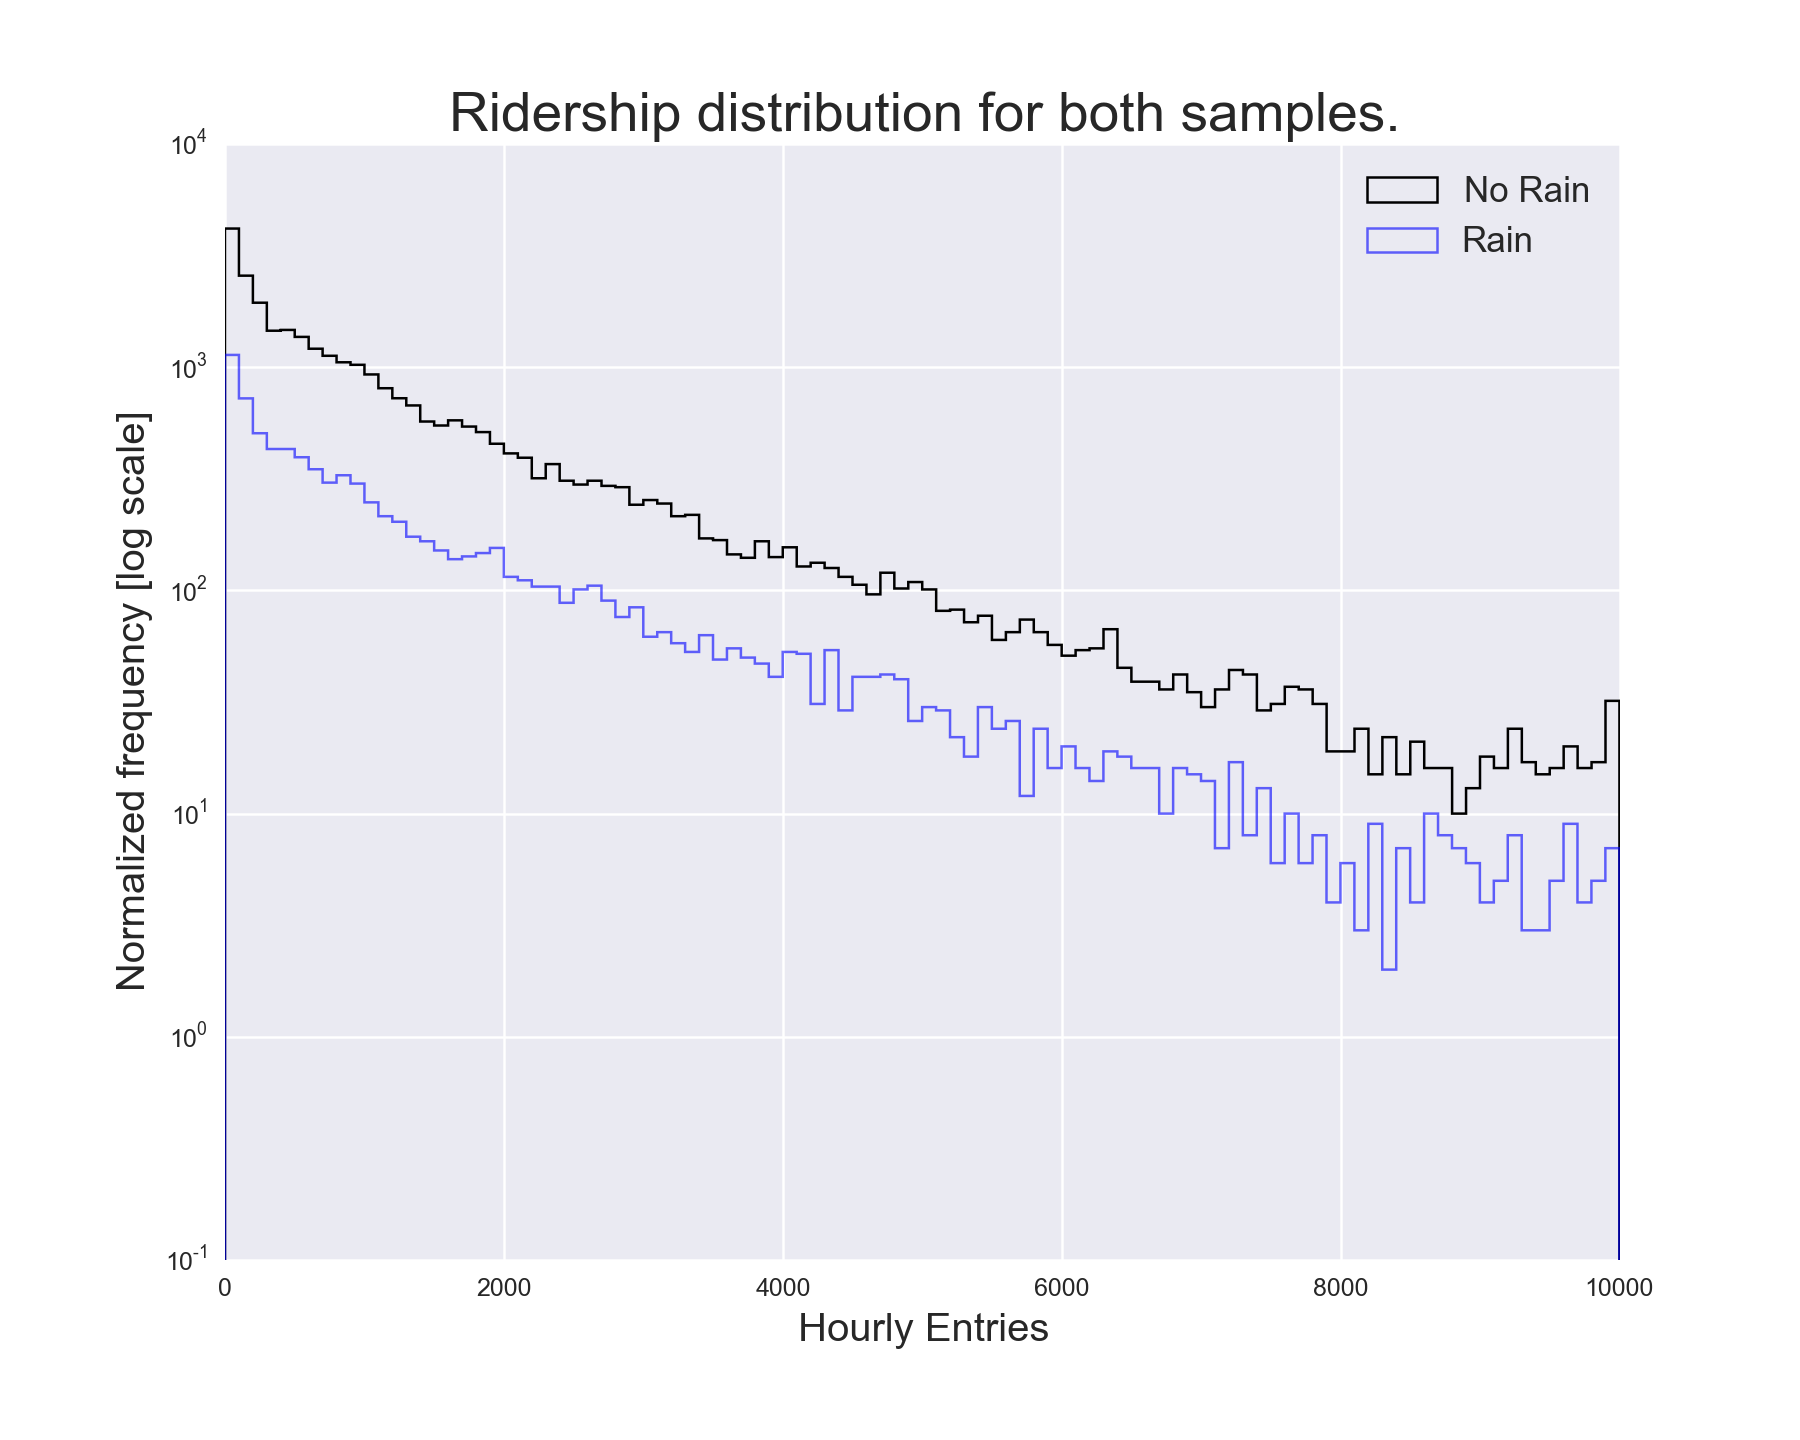
\includegraphics{samples_compared_nonnor.png}}
\caption{Ridership distribution comparison between rainy and dry days.}{\small 
Please note the logarithmic scale on axis Y. It was used to allows us to
study the visualization with more detail. Both distributions are similar in
shape, but the rainy sample is smaller than the rain sample (there was
precipitation reported for only 7 days of May 2011), and thus the counts
by bin are smaller.
}\label{section3:figure41}\end{figure}


\section{Supporting visualizations}
\label{section3:supporting-visualizations}
\textbf{One visualization can be more freeform.}

We will shown here some of the other plots that were created while working on
this project, and that help to answer particulars questions we have, or to
explore the data. All the code that produced these plots can be found on the
accompanying IPython notebook.
\begin{figure}[htbp]
\centering
\capstart

\scalebox{0.800000}{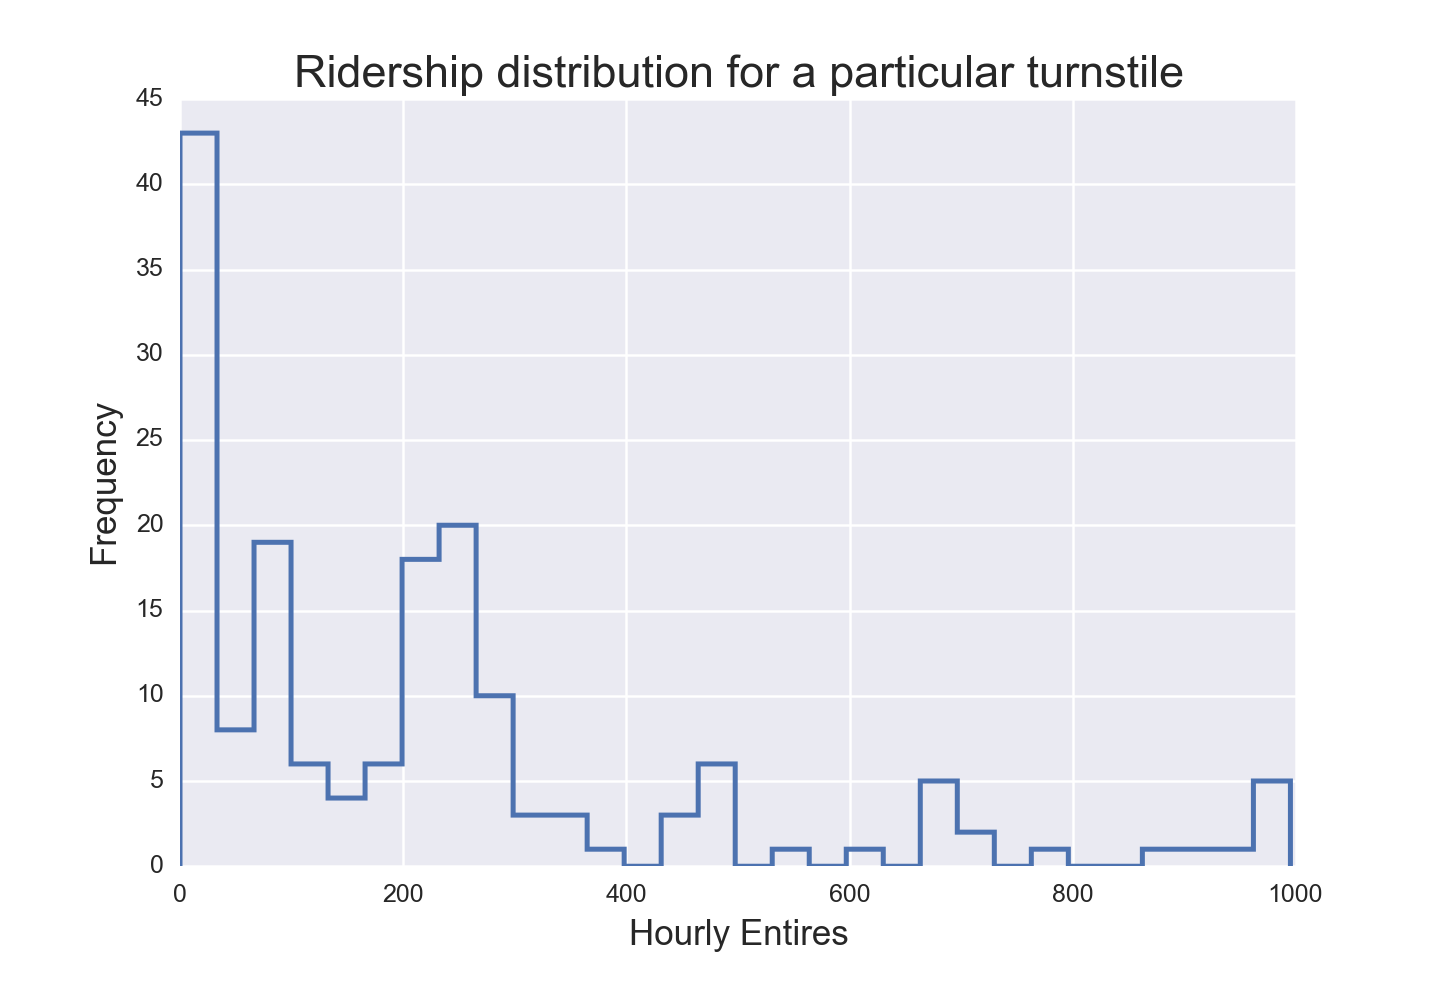
\includegraphics{viz1.png}}
\caption{Ridership distribution for one turnstile.}{\small 
With this figure we studied how the ridership distribution looked for the
data of one turnstile. It looks like there are multiple distributions within
the data (multiples modes), which correspond to the different distributions
for a particular hour and day of the week.
}\label{section3:figure42}\end{figure}
\begin{figure}[htbp]
\centering
\capstart

\scalebox{0.800000}{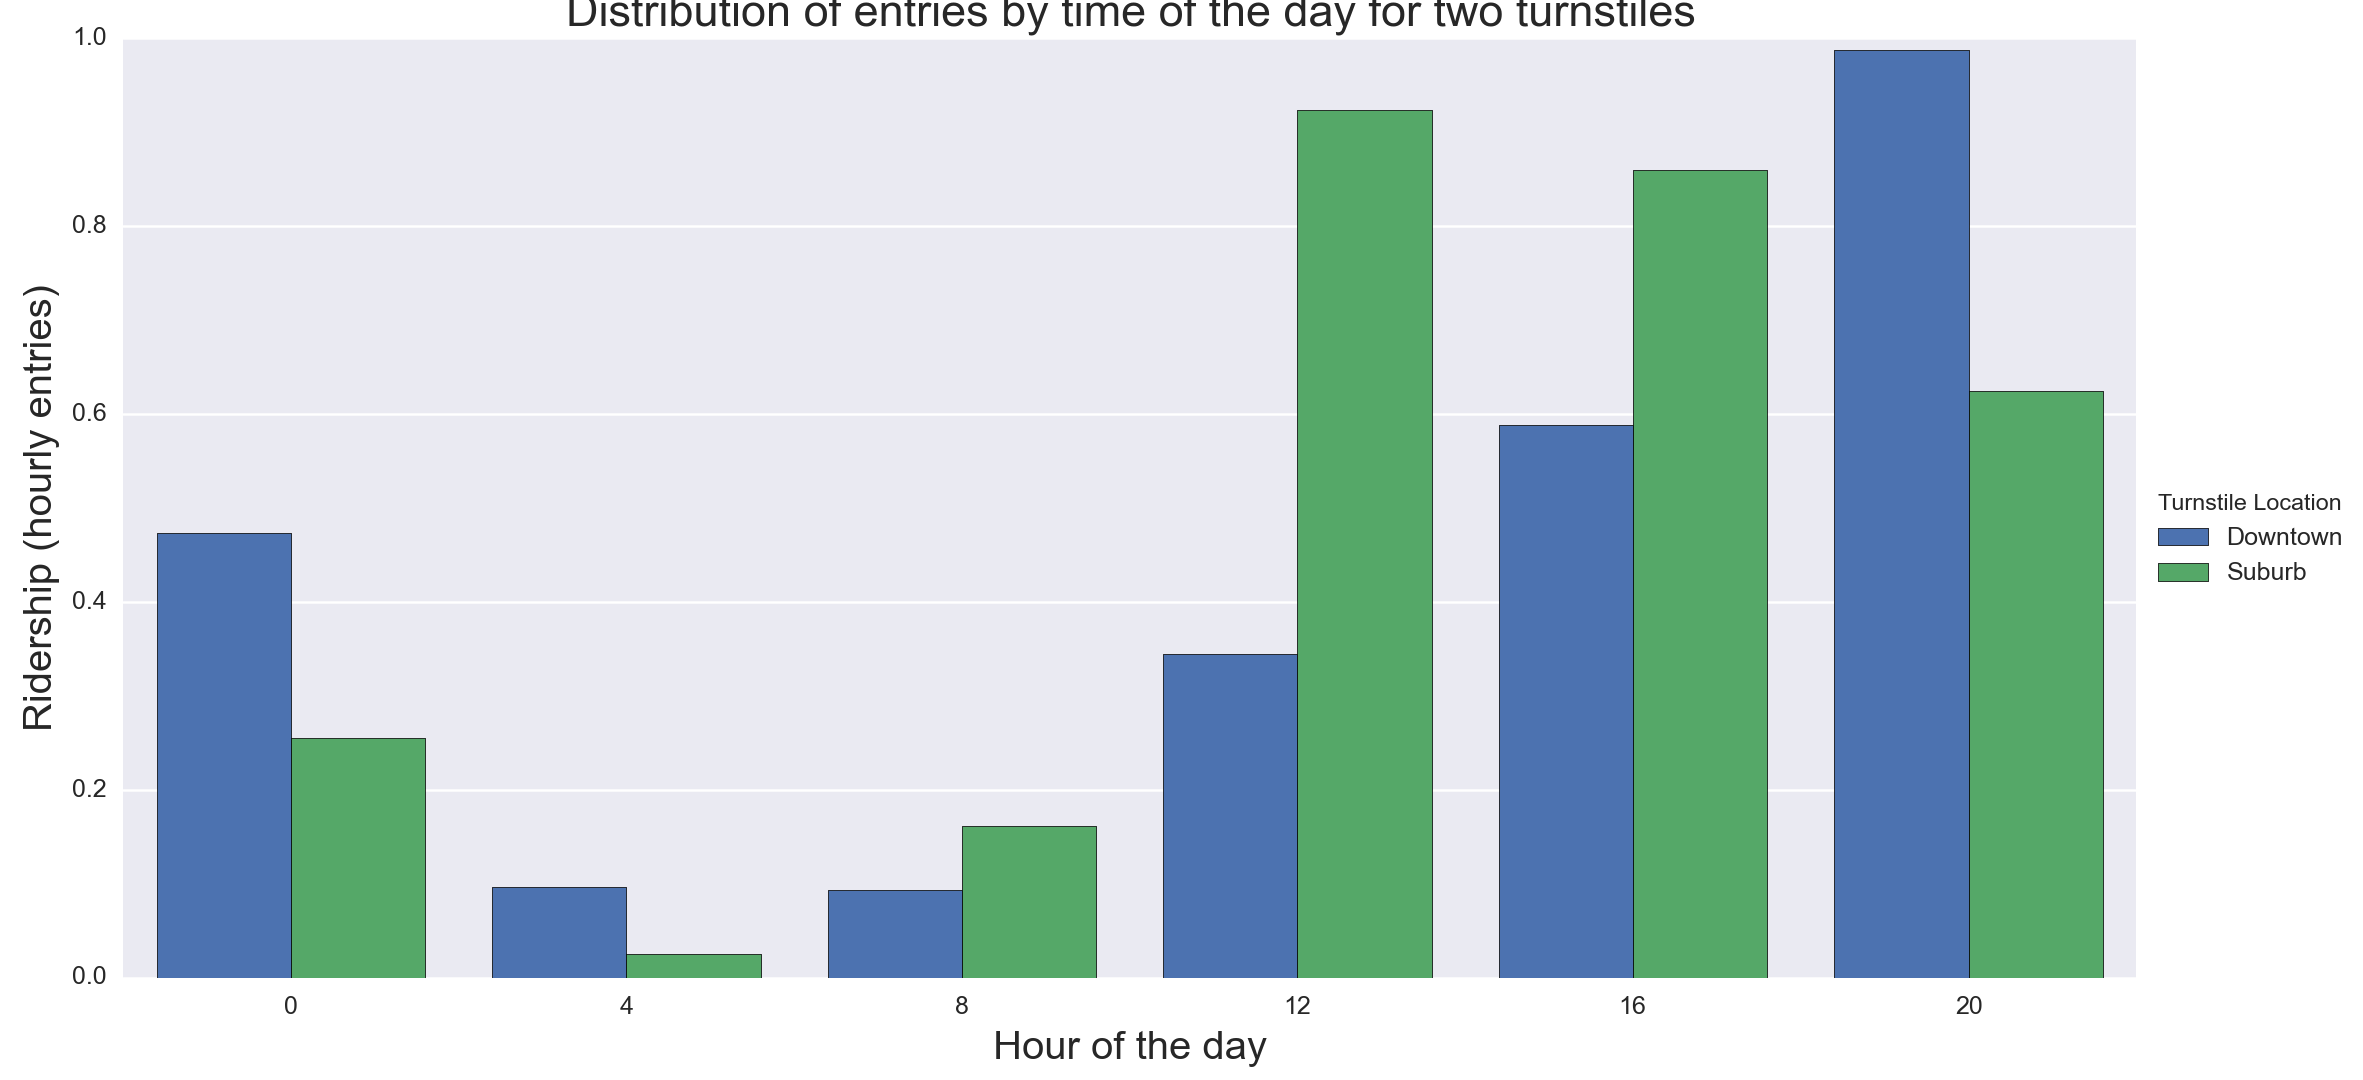
\includegraphics{viz2.png}}
\caption{Ridership behavior for two different turnstiles}{\small 
This plot was created to show the different daily behavior by turnstile
location, comparing one turnstile at downtown and other at the periphery. The
y-axis scale was normalized to focus on how different was the use of the
turnstiles along the day: the downtown locations tend to have a peak
at 20 hours, while the suburbs peak at noon.
}\label{section3:figure43}\end{figure}
\begin{figure}[htbp]
\centering
\capstart

\scalebox{0.800000}{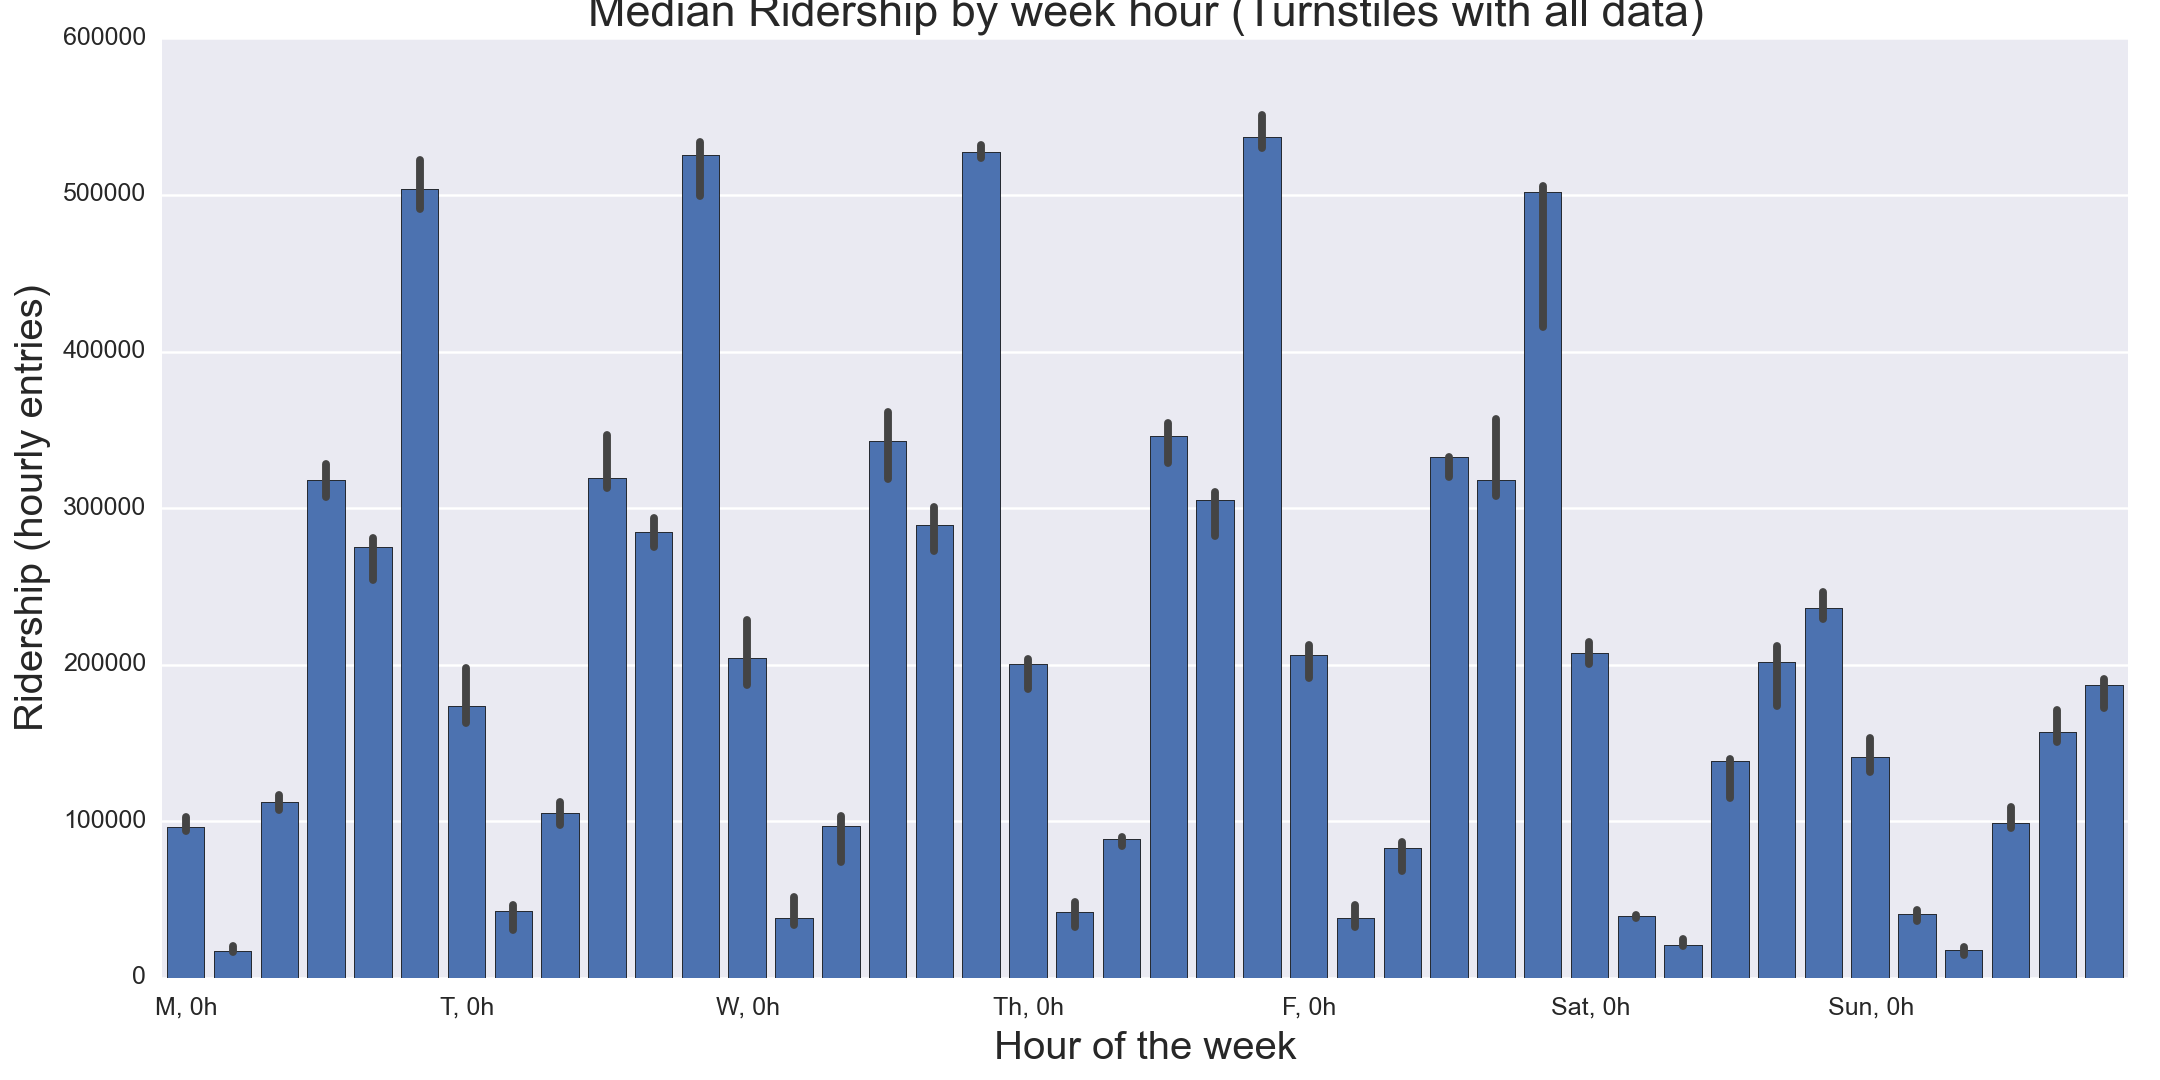
\includegraphics{viz3a.png}}
\caption{Weekly ridership behavior for turnstiles with no missing data.}{\small 
This figure, and the next, were created while studying the actual
independence of the rainy and non-rainy samples in chapter 2. We noticed
that several turnstiles within the original dataset didn't report information
for 1 or several times in May 2011, and we wanted to study what would happen
if we only worked with the complete turnstiles. We found out that the
locations with no missing data were mostly at downtown stations, and they
also represented mostly the busiest locations. Note that daily ridership
peaks at 20 hours. \emph{Notice that the x-axis includes markers for the 0 hours}
\emph{of each day of the week, and six reports happen each day, for 0, 4, 8, 12,}
\emph{16 and 20 hours.}
}\label{section3:figure44}\end{figure}
\begin{figure}[htbp]
\centering
\capstart

\scalebox{0.800000}{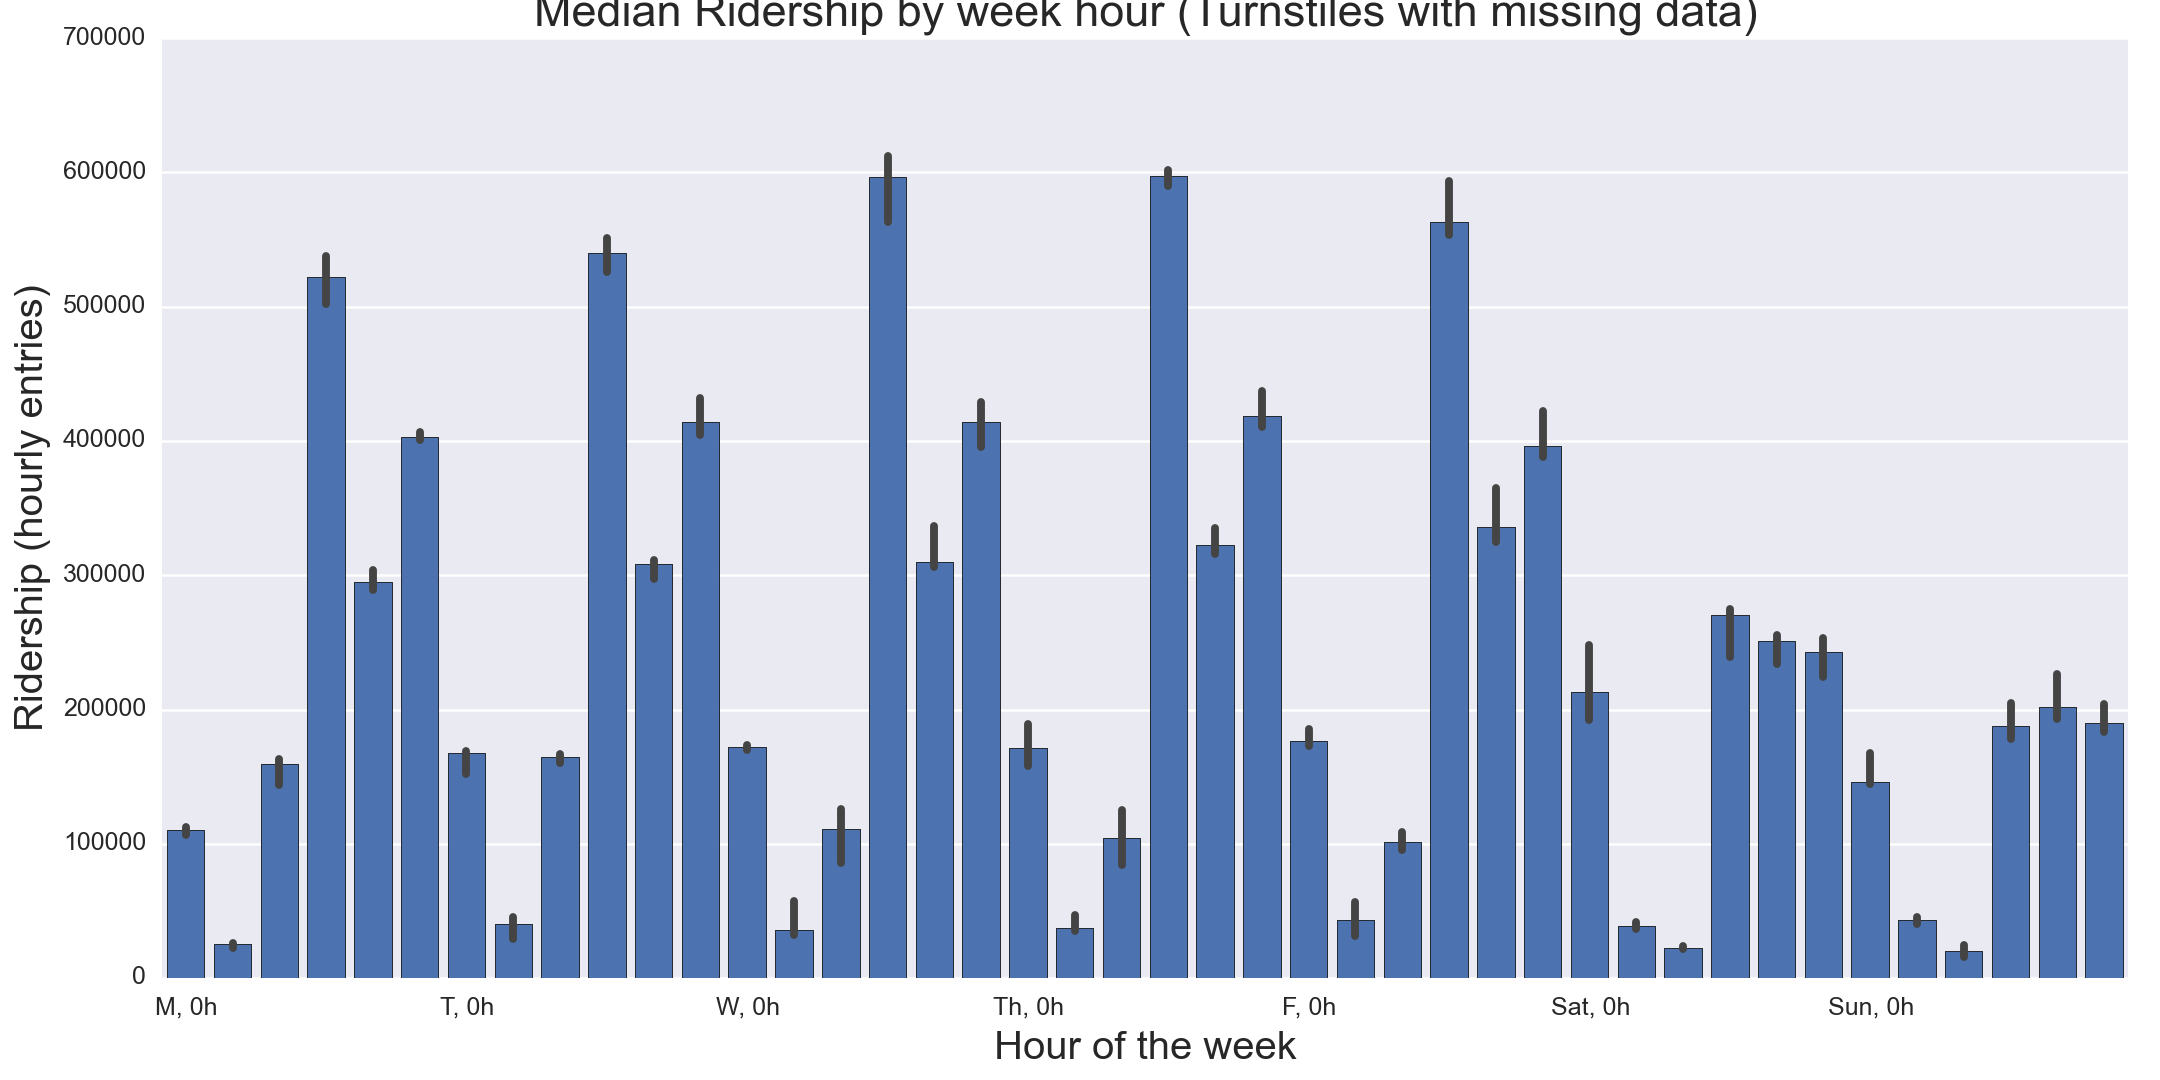
\includegraphics{viz3b.png}}
\caption{Weekly ridership behavior for turnstiles with missing data.}{\small 
Same as previous figure, but for data with missing data. Note how the daily
ridership behaviors changes, with two peaks, one at noon and the other at 20
hours. If a comparison is done with {\hyperref[section3:figure43]{\emph{Figure 4.3}}}, this sample
is more similar to the suburb station, while the previous sample is closer
to the behavior of the downtown locations.
}\label{section3:figure44b}\end{figure}
\begin{figure}[htbp]
\centering
\capstart

\scalebox{0.800000}{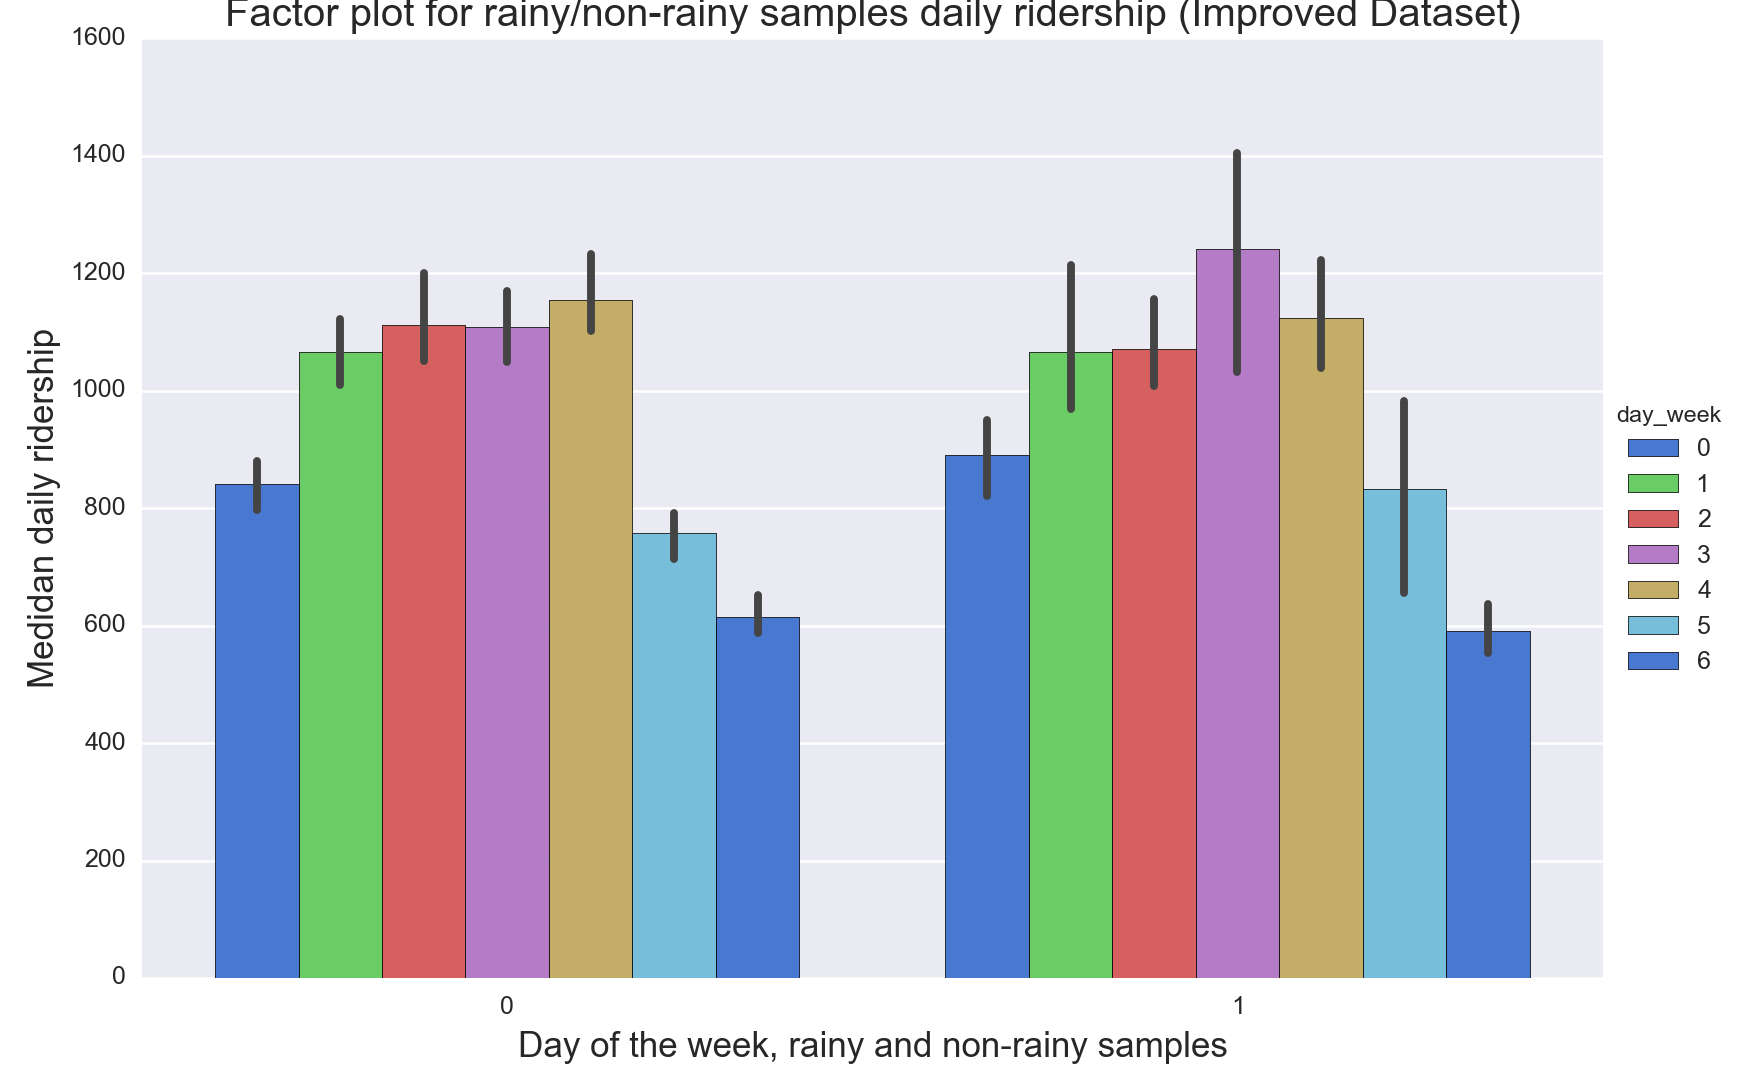
\includegraphics{viz4.png}}
\caption{Comparison of the daily ridership for non-rainy (0) and rainy (1) samples from
the improved dataset.}{\small 
This plots helps to compares how the ridership volume might be affected by the
precipitation conditions for each day of the week. Both samples seem too have
a pretty similar ridership volume for the same days, within the limits shown
by the 95\% confidence intervals (the black vertical lines in each bar)
}\label{section3:figure45}\end{figure}
\begin{figure}[htbp]
\centering
\capstart

\scalebox{0.800000}{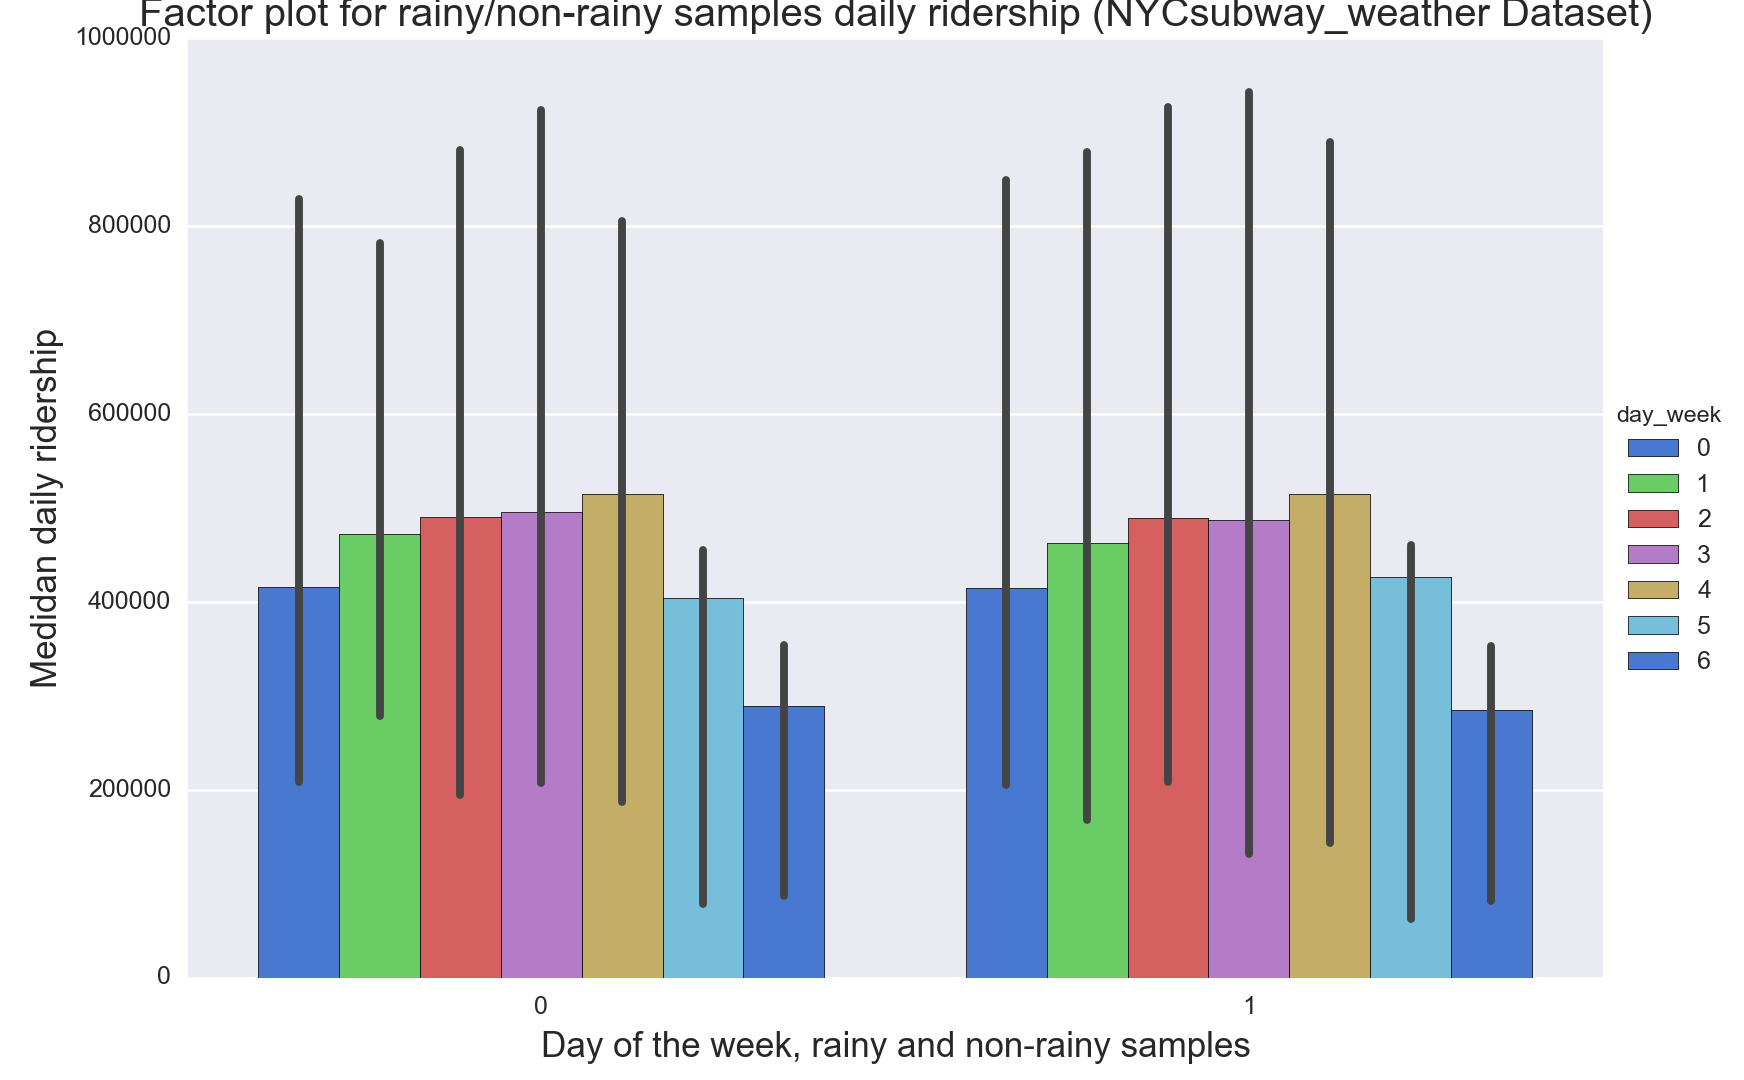
\includegraphics{viz5.png}}
\caption{Comparison of the daily ridership for non-rainy (0) and rainy (1) samples but
now from the \code{nycsubway\_weather} dataset.}{\small 
Same as previous figure. The daily ridership volume for both samples look even
more similar than in the previous plot. One drawback of this new dataset, that
treats the NYC subway system as a whole, is that we can notice that we do not
have too many data points to accurately study the ridership, as can be
seen by the big 95\% confidence interval lines. With most days having 4 (and
some 5) observed values within May 2011, when dividing between rainy and
non-rainy the number of observations drops even more.
}\label{section3:figure46}\end{figure}
\begin{figure}[htbp]
\centering
\capstart

\scalebox{0.800000}{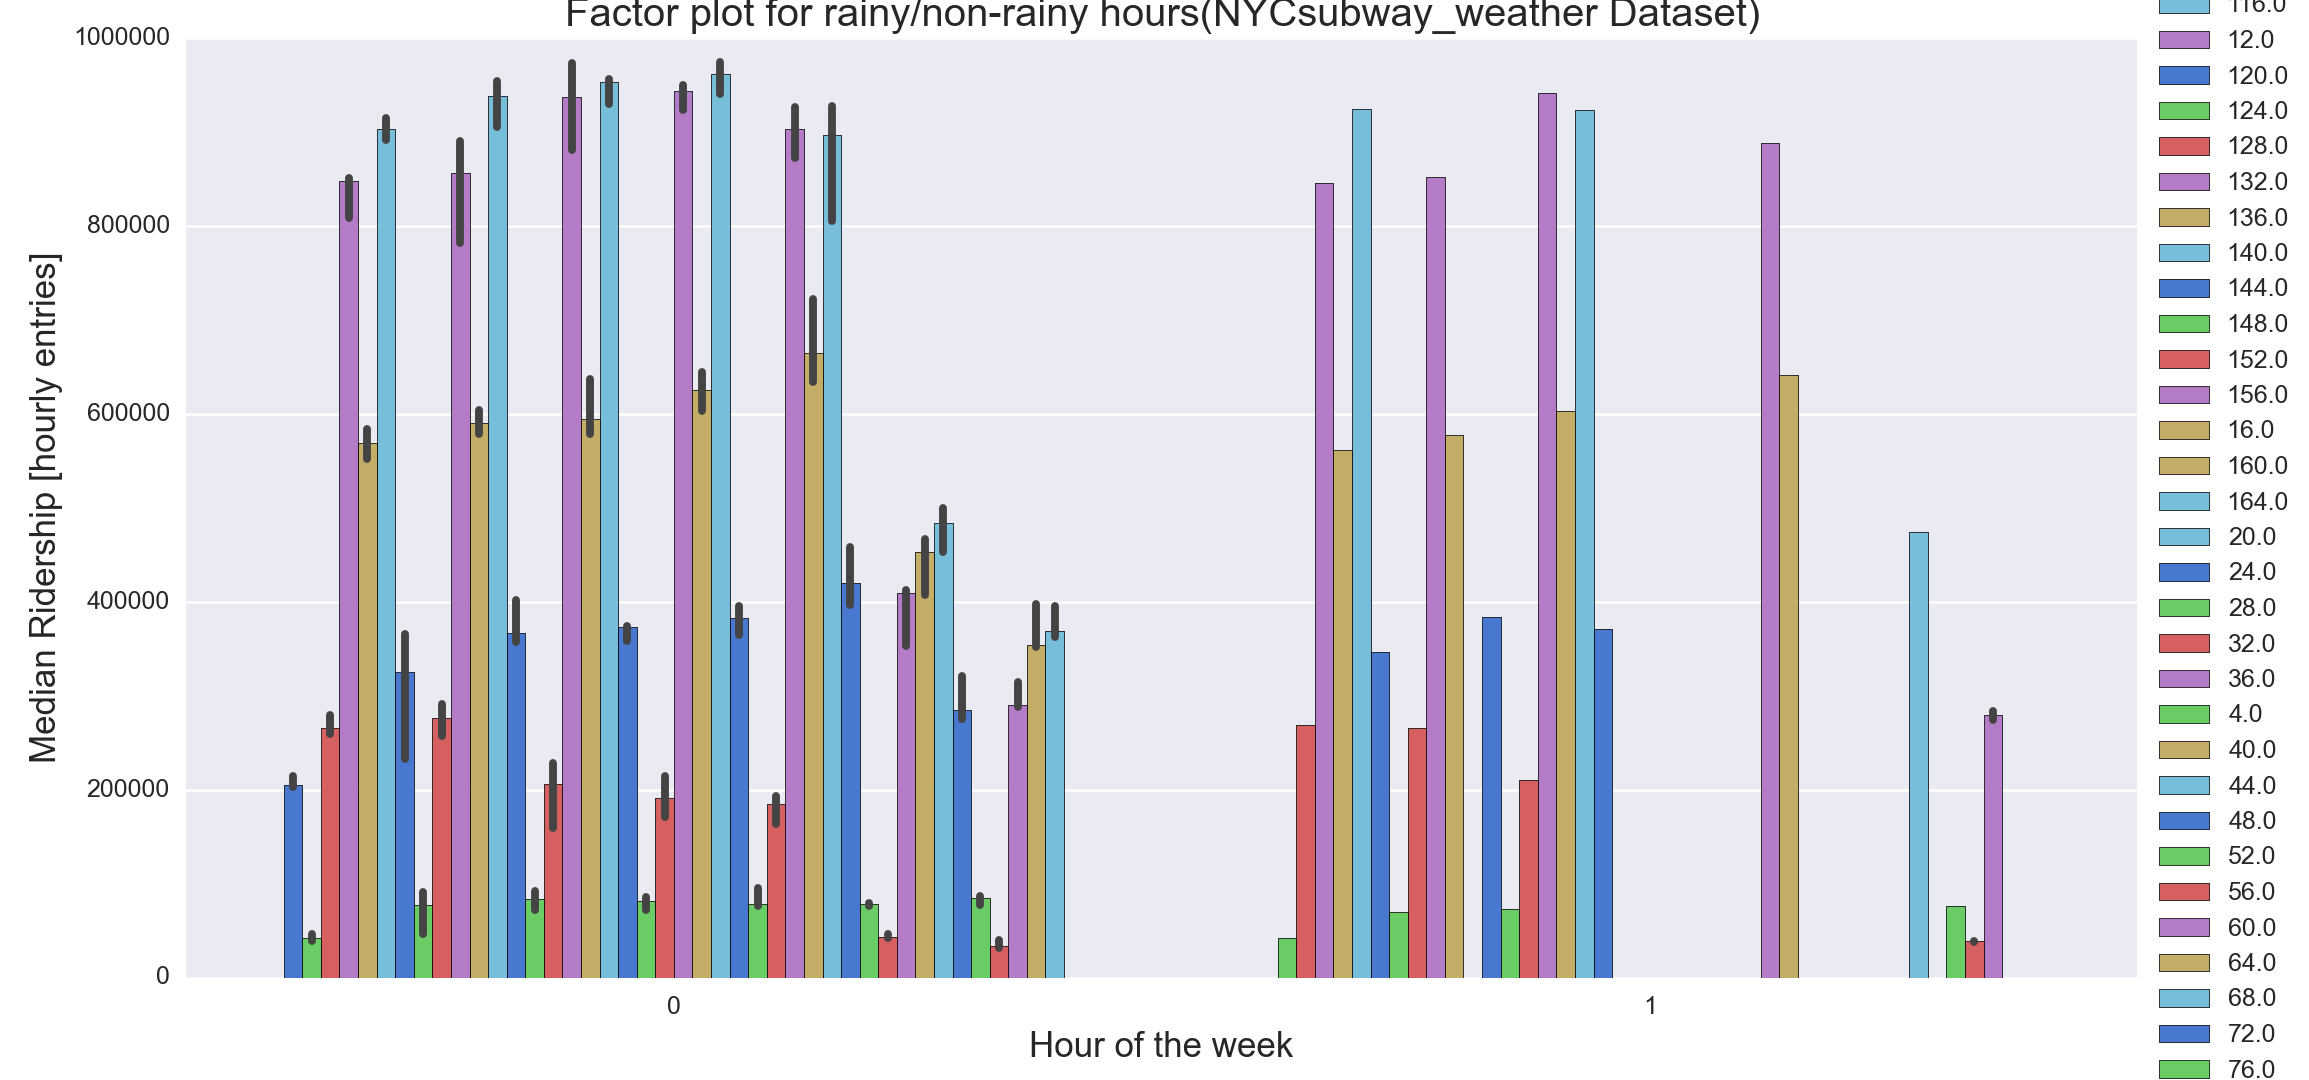
\includegraphics{viz6.png}}
\caption{Comparison of the week-hourly ridership volumes for the non-rainy and rainy
samples from the \code{nycsubway\_weather} dataset.}{\small 
This figure is similar to the previous two plots, but this time we use the
\code{rain\_hour} indicator to create the two samples. It is clearer now that we
might have not enough observations to answer the question behind this project,
does the ridership in the NYC subway changes with the rain conditions? \emph{Note}
\emph{that the x-axis, for each sample, shows values between 0 and 143, being 0}
\emph{the 0 hours of Monday, and 143 the 23 hours of Sunday}.
}\label{section3:figure47}\end{figure}


\chapter{Conclusions and Reflections}
\label{section4::doc}\label{section4:conclusions-and-reflections}

\section{Conclusion}
\label{section4:conclusion}
\textbf{From your analysis and interpretation of the data, do more people ride the}
\textbf{NYC subway when it is raining versus when it is not raining?  What analyses}
\textbf{lead you to this conclusion?}


\section{Shortcomings, limitations and insights}
\label{section4:shortcomings-limitations-and-insights}
\textbf{Please discuss potential shortcomings of the methods of your analysis}

\textbf{Do you have any other insight about the dataset that you would like to share}
\textbf{with us?}

\begin{thebibliography}{McKinney2013}
\bibitem[Diez2014]{Diez2014}{\phantomsection\label{overview:diez2014} 
Diez, Barr, Cetinkaya-Rundel. Introductory Statistics with
Randomizations and Simulation. 1st Edition. openintro.org
}
\bibitem[Diez2012]{Diez2012}{\phantomsection\label{overview:diez2012} 
Diez, Barr, Cetinkaya-Rundel. Open Intro Statistics. 2nd Edition.
openintro.org
}
\bibitem[McKinney2013]{McKinney2013}{\phantomsection\label{overview:mckinney2013} 
McKinney. Python for Data Analysis. 1st Edition.
O'Reilly Media. 2012.
}
\bibitem[Peck2012]{Peck2012}{\phantomsection\label{overview:peck2012} 
Peck, Olsen, Devore. Introduction to Statistics and Data Analysis.
4th Edition. Brooks/Cole. 2012.
}
\bibitem[Lyman2010]{Lyman2010}{\phantomsection\label{overview:lyman2010} 
Lyman Ott, Longnecker. An Introduction to Statistical Methods
and Data analysis. Sixth Edition. Brooks/Cole. 2010.
}
\bibitem[Rossant2014]{Rossant2014}{\phantomsection\label{overview:rossant2014} 
Rossant. IPython Interactive Computing and Visualization
Cookbook. 1st Edition. Packt Publishing. 2014.
}
\bibitem[glmscikit]{glmscikit}{\phantomsection\label{overview:glmscikit} 
\href{http://scikit-learn.org/stable/modules/linear\_model.html}{http://scikit-learn.org/stable/modules/linear\_model.html}
}
\bibitem[statsmodels]{statsmodels}{\phantomsection\label{overview:statsmodels} 
\href{http://statsmodels.sourceforge.net/stable/}{http://statsmodels.sourceforge.net/stable/}
}
\bibitem[wikiMann]{wikiMann}{\phantomsection\label{overview:wikimann} 
\href{http://en.wikipedia.org/wiki/Mann\%E2\%80\%93Whitney\_U\_test}{http://en.wikipedia.org/wiki/Mann\%E2\%80\%93Whitney\_U\_test}
}
\end{thebibliography}



\renewcommand{\indexname}{Index}
\printindex
\end{document}
